%==============================================================================
\documentclass[slovak,zadani]{components/fitthesis} % bez zadání - pro začátek práce, aby nebyl problém s překladem
%\documentclass[zadani]{fitthesis} % odevzdani do wisu - odkazy jsou barevné
%\documentclass[zadani,print]{fitthesis} % pro tisk - odkazy jsou černé
%\documentclass[zadani,cprint]{fitthesis} % pro barevný tisk - odkazy jsou černé, znak VUT barevný

% Základní balíčky jsou dole v souboru šablony fitthesis.cls
% zde muzeme vlozit vlastni balicky / you can place own packages here
\usepackage{graphicx}
\usepackage{subcaption}
\usepackage{multirow}
\usepackage{makecell}
\usepackage{dirtree}
\usepackage[]{algorithm2e}

%---rm---------------
\renewcommand{\rmdefault}{lmr}%zavede Latin Modern Roman jako rm / set Latin Modern Roman as rm
%---sf---------------
\renewcommand{\sfdefault}{qhv}%zavede TeX Gyre Heros jako sf
%---tt------------
\renewcommand{\ttdefault}{lmtt}% zavede Latin Modern tt jako tt

% vypne funkci šablony, která automaticky nahrazuje uvozovky,
% aby nebyly prováděny nevhodné náhrady v popisech API apod.
\csdoublequotesoff

% štýly ukážky kódu
\lstset {
    basicstyle=\small\ttfamily,
    frame=lrtb,
    numbers=left,
    stepnumber=1,
    showstringspaces=false,
    tabsize=1,
    breaklines=true,
    breakatwhitespace=false,
}

% štýl pre ukážky algoritmov
\RestyleAlgo{boxruled}

% citácia s autorovým menom
% \let\oldquote\quote
% \let\endoldquote\endquote
% \renewenvironment{quote}[2][]
%   {\if\relax\detokenize{#1}\relax
%      \def\quoteauthor{#2}%
%    \else
%      \def\quoteauthor{#2~---~#1}%
%    \fi
%    \oldquote}
%   {\par\nobreak\smallskip\hfill(\quoteauthor)%
%    \endoldquote\addvspace{\bigskipamount}}

% =======================================================================
% balíček "hyperref" vytváří klikací odkazy v pdf, pokud tedy použijeme pdflatex
% problém je, že balíček hyperref musí být uveden jako poslední, takže nemůže
% být v šabloně
\ifWis
\ifx\pdfoutput\undefined % nejedeme pod pdflatexem / we are not using pdflatex
\else
  \usepackage{color}
  \usepackage[unicode,colorlinks,hyperindex,plainpages=false,pdftex]{hyperref}
  \definecolor{links}{rgb}{0.4,0.5,0}
  \definecolor{anchors}{rgb}{1,0,0}
  \def\AnchorColor{anchors}
  \def\LinkColor{links}
  \def\pdfBorderAttrs{/Border [0 0 0] }  % bez okrajů kolem odkazů / without margins around links
  \pdfcompresslevel=9
\fi
\else % pro tisk budou odkazy, na které se dá klikat, černé / for the print clickable links will be black
\ifx\pdfoutput\undefined % nejedeme pod pdflatexem / we are not using pdflatex
\else
  \usepackage{color}
  \usepackage[unicode,colorlinks,hyperindex,plainpages=false,pdftex,urlcolor=black,linkcolor=black,citecolor=black]{hyperref}
  \definecolor{links}{rgb}{0,0,0}
  \definecolor{anchors}{rgb}{0,0,0}
  \def\AnchorColor{anchors}
  \def\LinkColor{links}
  \def\pdfBorderAttrs{/Border [0 0 0] } % bez okrajů kolem odkazů / without margins around links
  \pdfcompresslevel=9
\fi
\fi
% Řešení problému, kdy klikací odkazy na obrázky vedou za obrázek
\usepackage[all]{hypcap}

% Informace o práci/projektu / Information about the thesis
%---------------------------------------------------------------------------
\projectinfo{
  %Prace / Thesis
  project=BP,            %typ prace BP/SP/DP/DR  / thesis type (SP = term project)
  year=2018,             %rok odevzdání / year of submission
  date=\today,           %datum odevzdani / submission date
  %Nazev prace / thesis title
  title.cs={Mobilná aplikácia pre akvizíciu a úpravu\\HDR fotografií},
  %nazev prace v cestine ci slovenstine (dle zadani) / thesis title in czech language (according to assignment)
  title.en={Mobile application for acquisition and editing HDR images},
  %nazev prace v anglictine / thesis title in english
  %Autor / Author
  author={Patrik Michalák},   %cele jmeno a prijmeni autora / full name and surname of the author
  author.name={Patrik},   %jmeno autora (pro citaci) / author name (for reference) 
  author.surname={Michalák},   %prijmeni autora (pro citaci) / author surname (for reference) 
  %author.title.p=Bc., %titul pred jmenem (nepovinne) / title before the name (optional)
  %author.title.a=PhD, %titul za jmenem (nepovinne) / title after the name (optional)
  %Ustav / Department
  department=UPGM, % doplnte prislusnou zkratku dle ustavu na zadani: UPSY/UIFS/UITS/UPGM
  %Skolitel / supervisor
  supervisor=Martin Čadík, %cele jmeno a prijmeni skolitele / full name and surname of the supervisor
  supervisor.name={Martin},   %jmeno skolitele (pro citaci) / supervisor name (for reference) 
  supervisor.surname={Čadík},   %prijmeni skolitele (pro citaci) / supervisor surname (for reference) 
  supervisor.title.p={Doc. Ing.},   %titul pred jmenem (nepovinne) / title before the name (optional)
  supervisor.title.a={Ph.D.},    %titul za jmenem (nepovinne) / title after the name (optional)
}

%Abstrakt (cesky, slovensky ci anglicky) / Abstract (in czech, slovak or english)
\abstract[cs]{Hlavnou myšlienkou tejto práce je vytvoriť aplikáciu, ktorá by riešila nielen problémy generovania a spracovania
  HDR obsahu, ale zamerala sa aj na interakciu s užívateľom a poskytla mu viac možností v prehľadnom a minimalistickom
  rozhraní. V riešení bola použitá metóda generovania HDR obsahu kombinovaním LDR snímok
	s rôznou hodnotou času expozície. Vytvorené riešenie poskytuje užívateľovi mobilnú aplikáciu pre prácu
	s HDR fotografiou, štyri metódy mapovania tónov a rôzne nástroje, ktoré užívateľ pri práci potrebuje.
}
\abstract[en]{The goal of this paper is to create an application that solves HDR image processing problems and focuses
  to interactivity with the user, offering him more opportunities in clear and minimalistic graphic user interface.
  Application generate HDR content by merging a series of low dynamic range images with different exposure time
  values. The solution provides work with HDR photography, four tone mapping methods and various tools for user.
}

%Klicova slova (cesky, slovensky ci anglicky) / Keywords (in czech, slovak or english)
\keywords[cs]{digitálna fotografia, spracovanie obrazu, mobilná aplikácia, vysoký dynamický rozsah,\\mapovanie tónov}
\keywords[en]{digital photography, image processing, mobile application, high dynamic range, tone\\mapping}

%Prohlaseni (u anglicky psane prace anglicky, u slovensky psane prace slovensky)
\declaration{Prehlasujem, že som túto bakalársku prácu vypracoval samostatne pod vedením pána docenta Ing. Martina Čadíka, Ph.D.
Uviedol som všetky literárne pramene a publikácie, z~ktorých som čerpal.}

%Podekovani (nepovinne, nejlepe v jazyce prace) / Acknowledgement (optional, ideally in the language of the thesis)
\acknowledgment{Rád by som poďakoval pánovi docentovi Ing. Martinovi Čadíkovi, Ph.D. za odbornú pomoc, pripomienky a rady
poskytnuté počas tvorby tejto práce. Taktiež ďakujem za podporu pri~kvalifikácii a konečnej prezentácii práce
na konferencii Excel@FIT 2018. Za úvodnú motiváciu a pomoc ďakujem Ing. Romanovi Tábimu, zásluhou ktorého už matematické
funkcie nie sú až tak náročné.}

% řeší první/poslední řádek odstavce na předchozí/následující stránce
\clubpenalty=10000
\widowpenalty=10000

\begin{document}
  % Vysazeni titulnich stran / Typesetting of the title pages
  % ----------------------------------------------
  \maketitle
  % Obsah
  % ----------------------------------------------
  \setlength{\parskip}{0pt}

  {\hypersetup{hidelinks}\tableofcontents}
  
  % Seznam obrazku a tabulek (pokud prace obsahuje velke mnozstvi obrazku, tak se to hodi)
  \ifczech
    \renewcommand\listfigurename{Seznam obrázků}
  \fi
  \ifslovak
    \renewcommand\listfigurename{Zoznam obrázkov}
  \fi
  % \listoffigures
  
  \ifczech
    \renewcommand\listtablename{Seznam tabulek}
  \fi
  \ifslovak
    \renewcommand\listtablename{Zoznam tabuliek}
  \fi
  % \listoftables 

  \ifODSAZ
    \setlength{\parskip}{0.5\bigskipamount}
  \else
    \setlength{\parskip}{0pt}
  \fi

  % vynechani stranky v oboustrannem rezimu
  % Skip the page in the two-sided mode
  \iftwoside
    \cleardoublepage
  \fi

  % Text prace
  % ----------------------------------------------
  \chapter{Úvod}
Okolie, ktoré vnímame, má vysoký dynamický rozsah svetla a farieb. Tmavé miesta bez osvetlenia neobsahujú takmer žiaden jas a naopak
scéna zameraná na zdroj svetla obsahuje priveľmi veľa jasu. Ľudské oko je schopné prispôsobiť sa takýmto zmenám a pozorovať detaily
aj na scéne s rozmanitým rozsahom jasu.

Väčšina digitálnych fotoaparátov a zobrazovacích zariadení však zachytávajú a zobrazujú farebné obrázky ako matice 24-bitových pixelov,
v ktorých je obsiahnutých 8-bitov v~rozsahu 0 až 255 pre každý farebný kanál. Preto sa digitálne fotoaparáty pokúšajú odhadnúť osvetlenie
a automaticky nastaviť čas expozície tak, aby mal najdôležitejší aspekt scény čo najlepší dynamický rozsah a jas miest, ktoré sú príliš
tmavé, alebo naopak príliš svetlé, je orezaný na hodnoty 0 a 255. Tento problém rieši HDR fotografia, avšak nie veľa bežných užívateľov si
je vedomých, čo to vlastne HDR fotografia znamená a ako sa s ňou pracuje.

HDR fotografia umožňuje zachytiť veľkú časť rozsahu jasu reálneho sveta a následnú prácu s týmito dátami. Existuje viacero mobilných aplikácií,
ktoré ponúkajú vytvorenie a~spracovanie HDR fotografie. Veľa verejne dostupných aplikácií však používa iba filter aplikovaný na jednu
fotografiu, ktorý zvýši kontrast farieb a detaily a tým sa snaží opticky vytvoriť efekt HDR. Na druhej strane sú aplikácie, ktoré
vytvárajú HDR fotografiu skladaním série snímok s rôznymi nastaveniami času expozície. Tieto aplikácie však poväčšine užívateľovi neposkytujú
dostatočne záživné užívateľské rozhranie, majú pre užívateľa veľmi obmedzené možnosti, alebo sa s nimi ťažko a neintuitívne pracuje.

Zameraním tejto práce je vytvoriť aplikáciu, ktorá by riešila nielen problémy generovania a spracovania HDR obsahu, ale zamerala sa aj na
interakciu s užívateľom a poskytla mu viac možností ako bežná aplikácia. Každá scéna je niečim výnimočná a jednoduché východzie nastavenia
hodnôt parametrov nedosiahnú vždy uspokojivé výsledky.


\chapter{Teoretická časť}
\section{Svetlo}

Viditeľné svetlo je forma energie pohybujúca sa v priestore, vzájomne pôsobiaca
s materiálmi, kde môže byť absorbovaná, lomená, odrazená alebo prenesená.

Ľudské oko dokáže zachytiť svetlo, ktorého výsledkom je stimulovanie oka k vytvoreniu
vizuálnych obrazov, závislých na vlnovej dĺžke. Vlnové dĺžky viditeľné ľudským okom
majú hodnoty od 380 do 780 nm. \cite{AHDR}

\subsection*{Rádiometria}

Veda zameraná na meranie svetla sa nazýva rádiometria. Pri meraní svetla nás zaujímajú
jeho vlastnosti šírenia priestorom, vzduchom, vodou a materiálmi. Energiu meriame v čase,
priestore alebo uhle.

\begin{description}
    % irradiance
    \item [Ožiarenie] je množstvo energie dopadajúce na jedno miesto z rôznych zdrojov a smerov.
    % radiance exitance
    \item [Žiarenie zdroja] je energia vyžarujúca z jedného bodu do všetkých prístupných smerov.
    % radiant intensity
    \item [Intenzita žiarenia] je energia vyžarovaná zo zdroja v jeden daný smer. Je meraná ako
    jednotka energie za jednotku času za jednotku uhlu smeru.
    % radiance
    \item [Žiarenie] je energia dopadajúca na jedno miesto z určitého smeru a v určitom uhle.
    Je to množstvo energie prenášané za jednotku času za jednotku plochy a za jednotku smeru.
\end{description}

\begin{figure}[h!]
    \centering
    \begin{subfigure}{0.2\textwidth}
        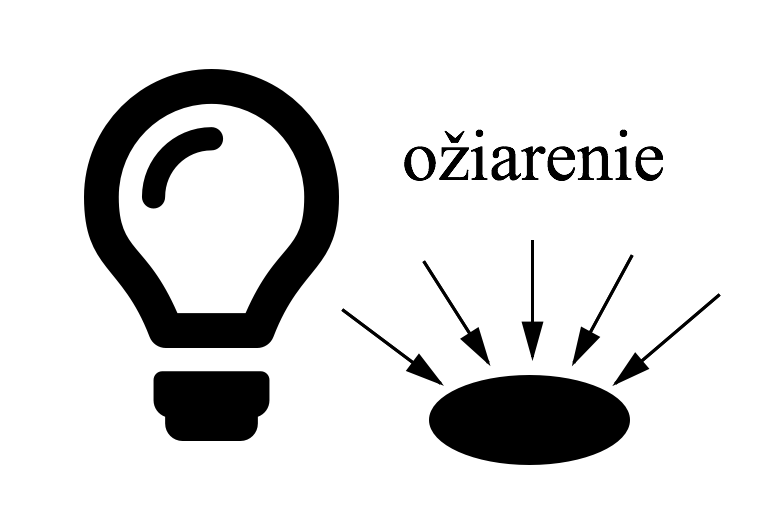
\includegraphics[width=\textwidth]{figures/light/irradiance}
    \end{subfigure}
    ~
    \begin{subfigure}{0.2\textwidth}
        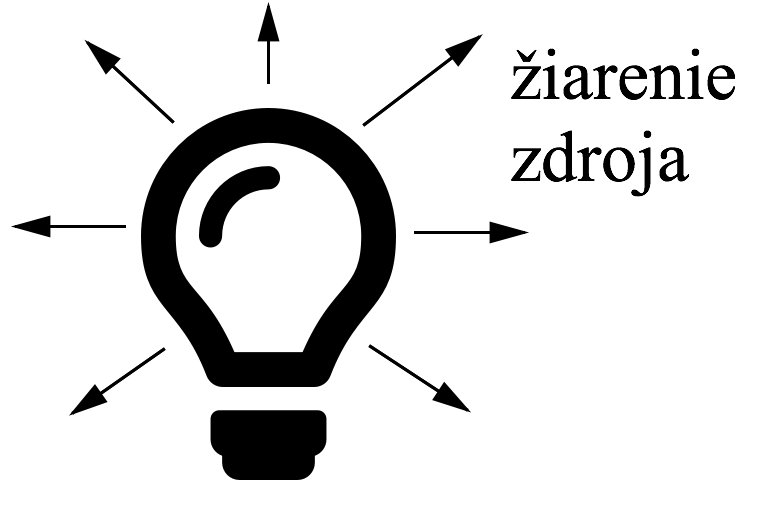
\includegraphics[width=\textwidth]{figures/light/radiant_exitance}
    \end{subfigure}
    ~
    \begin{subfigure}{0.2\textwidth}
        
\includegraphics[width=\textwidth]{figures/light/radiant_intensity}
    \end{subfigure}
    ~
    \begin{subfigure}{0.2\textwidth}
        
\includegraphics[width=\textwidth]{figures/light/radiance}
    \end{subfigure}
    \caption{Rádiometrické veličiny}
    \label{fig:radiometry}
\end{figure}

Základým faktorom tvorby fotografie je svetlo dopadajúce na povrch z určitého smeru.
Pri vytváraní fotografie sa uzávierka fotoaparátu na malý čas otvorí a prepustí do vnútra 
fotoaparátu svetlo. Tomuto času hovoríme čas expozície. Dĺžka expozičného času určuje,
koľko svetla prenikne do tela fotoaparátu.
Šošovka fotoaparátu obmedzuje smer, z ktorého je svetlo prijímané.
Senzor je rozdelený na malé oblasti pixelov, kde každá oblasť zaznamená svetlo pre danú plochu.

\subsection*{Fotometria}

Fotometria je odbor optiky, ktorý skúma svetlo z pohľadu jeho pôsobenia na ľudské vnímanie.
Povrchy materiálov odrážajú svetlo a tým môžu pozmeniť jeho spektrálnu kompozíciu.
Následne odrazené svetlo nesie informáciu zároveň o zdroji svetla osvetľujúceho
povrch a~o~odrazivosti povrchu na danom mieste.

\begin{description}
    % luminosity
    \item [Svietivosť] je základnou fotometrickou veličinou. Svietivosť vyjadruje množstvo
    svetelného toku vyslaného zdrojom do priestorového uhla a je analogická intenzite žiarenia.
    % illuminance - osvetlenie
    \item [Osvetlenie] je definované ako svetelný tok dopadajúci na jednotku plochy a je analogické
    ožiareniu.
    % luminance
    \item [Jas] je fotometrická veličina vyjadrujúca intenzitu svietivosti pre jednotku plochy
    v určitom smere.
\end{description}

Jas kladie prirodzené hranice viditeľnosti vlnových dĺžok, čo je dôležité pre HDR.
Vlnové dĺžky nachádzajúce sa mimo rozsahu viditeľnosti nemusia byť zaznamenávané, ukladané a~ani
spracované. Základom väčšiny operátorov pre mapovanie tonality je počiatočné extrahovanie hodnôt
jasu každého pixelu podľa zložiek RGB pred zredukovaním dynamického rozsahu, pretože na vnímanie
majú väčší vplyv rozdiely v rozsahu jasu ako kontrast farieb.

\subsection*{Farebné priestory}

\begin{figure}[t]
    \centering
    \begin{subfigure}{0.54\textwidth}
        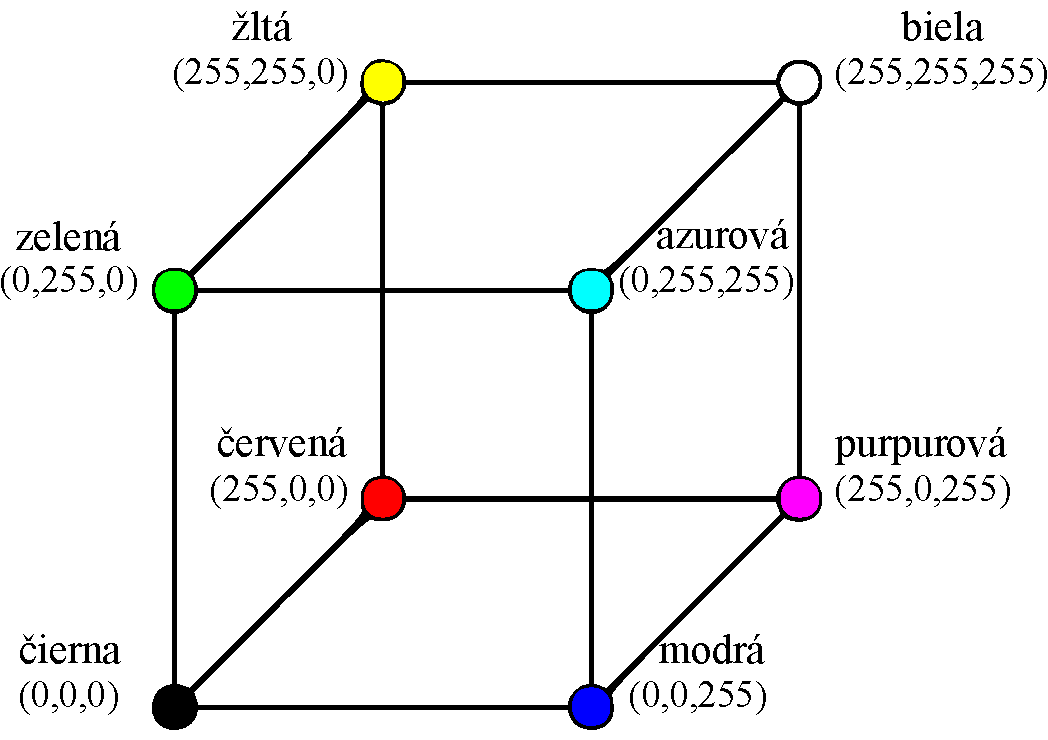
\includegraphics[width=\textwidth]{figures/light/rgb}
        \caption{RGB kocka}
        \label{fig:colorModels_rgb}
    \end{subfigure}
    ~
    \begin{subfigure}{0.35\textwidth}
        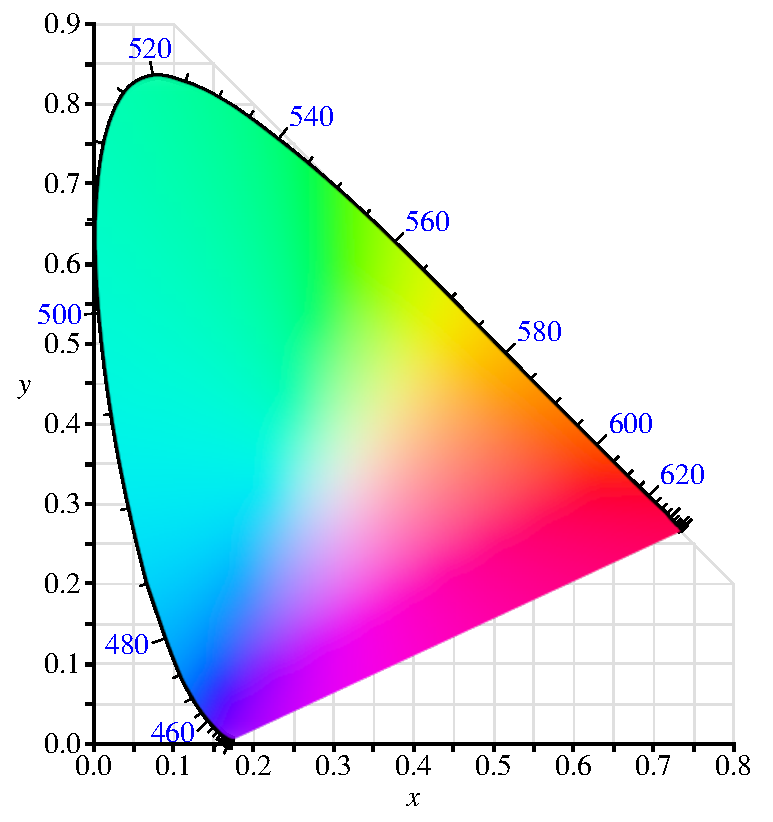
\includegraphics[width=\textwidth]{figures/light/cie}
        \caption{Chromatický diagram CIE}
        \label{fig:colorModels_cie}
    \end{subfigure}
    \caption{Grafická reprezentácia farebných priestorov \cite{AHDR}}
    \label{fig:colorModels}
\end{figure}

Farebný model popisuje reprezentáciu farieb ako $n$-ticu číselných hodnôt. Farba je väčšinou reprezentovaná troma alebo štyrmi farebnými
zložkami. Farebný priestor určuje rozsah farieb pre viditeľné spektrum.

\subsection*{sRGB}

Model RGB je založený na aditívnom miešaní primárnych farebných zložiek (červená, zelená a modrá), z ktorých každá stimuluje jeden z troch
farebných receptorov ľudského oka. Kombináciami týchto troch farebných zložiek obsiahneme značnú časť farebného priestoru, ktorý je človek
schopný vnímať. Žiaľ, neexistujú štandardy, ktoré by definovali aké hodnoty musia mať tieto základné farebné zložky, preto sa môžu rovnaké
hodnoty RGB na rozličných obrazovkách mierne líšiť. Farebný priestor tohoto modelu je možné reprezentovať v tzv. RGB kocke (obr.
\ref{fig:colorModels_rgb}). Akýkoľvek bod v kocke predstavuje farbu zloženú z farebných kanálov reprezentovaných 8 alebo 16-bitovou hodnotou.

\subsection*{CIE XYZ}

CIE XYZ je jedným z prvých matematicky definovaných farebných priestorov, ktorý je odvodený podľa vlastností ľudského oka. Každú farbu modelu
je možné presne matematicky popísať. Jedným spôsobom je popísať množstvo trichromatických zložiek, označovaných ako X, Y a Z. Výsledok dostaneme
integráciou spektrálneho farebného podnetu a trichromatických členov v celom rozsahu viditeľného spektra. Druhým spôsobom je vyjadriť 
tzv. trichromatické súradnice pomocou normových podielov.

V praxi sa využívajú na vyjadrenie chromatickosti farby iba zložky X a Y. V takom prípade je možné používať tzv. chromatický diagram (obr.
\ref{fig:colorModels_cie}).

\section{Snímanie}

\begin{figure}[t]
    \centering
    \begin{subfigure}{0.3\textwidth}
        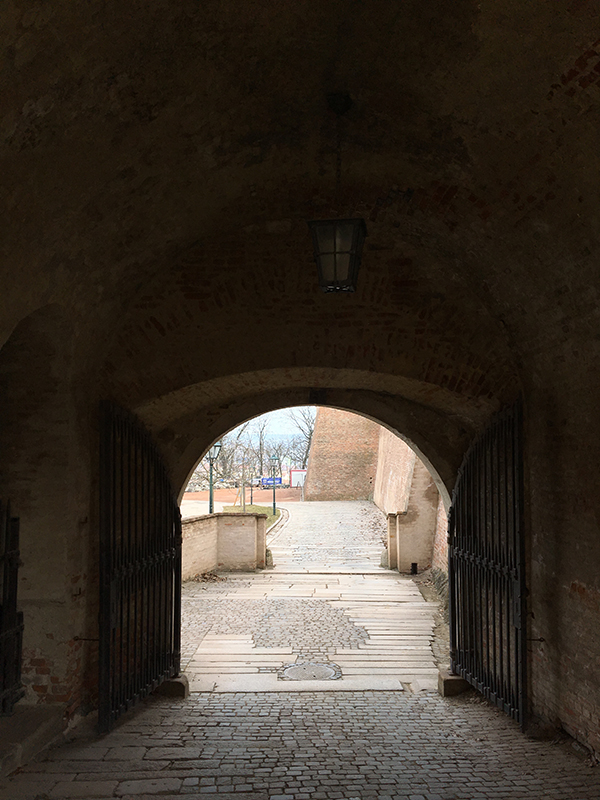
\includegraphics[width=\textwidth]{figures/capturing/exposures/underexposed}
        \caption{podexponovaná scéna}
        \label{fig:underexposed}
    \end{subfigure}
    ~
    \begin{subfigure}{0.3\textwidth}
        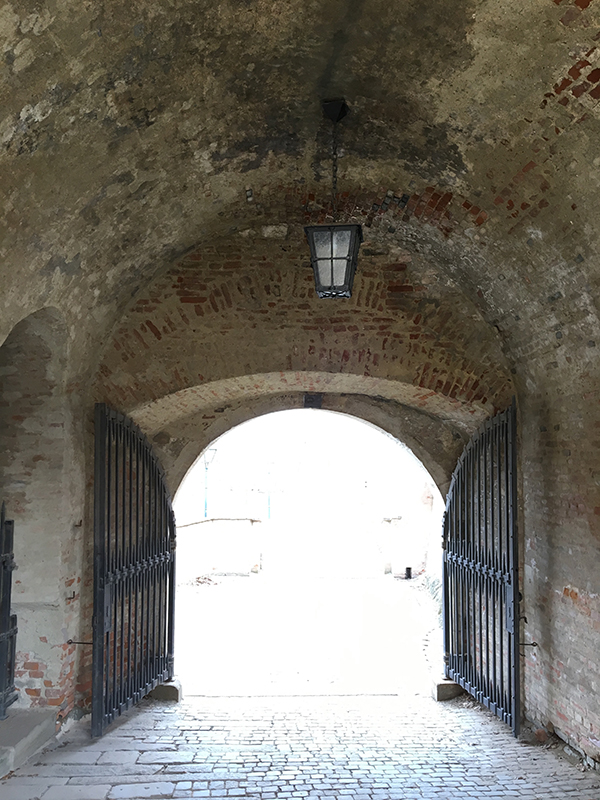
\includegraphics[width=\textwidth]{figures/capturing/exposures/overexposed}
        \caption{preexponovaná scéna}
        \label{fig:overexposed}
    \end{subfigure}
    \caption{Rozličné expozície rovnakej scény}
    \label{fig:exposed_scene}
\end{figure}

Je veľmi obtiažne zachytiť scénu (obr. \ref{fig:exposed_scene}), kde sú svetlé miesta mnohonásobne jasnejšie ako
tmavé miesta scény. To znamená, že takáto scéna má vysoký dynamický rozsah.
Rozličné nastavenia času expozície nám umožňujú vytvoriť fotografiu zachytávajúcu

a) veľmi svetlé (obr. \ref{fig:underexposed}) alebo

b) veľmi tmavé oblasti (obr. \ref{fig:overexposed}).

Na obrázku \ref{fig:pipeline} sú zobrazené technológie, ktorými je možné snímať, generovať
a zobrazovať scény s vysokým dynamickým rozsahom. Prvým problémom je zachytenie dynamického 
rozsahu scény. V súčasnosti existujú 3 metódy vytvárania HDR obsahu:
\begin{itemize}
    \item kombinovaním LDR snímok s rôznou hodnotou času expozície (obr. \ref{fig:pipeline} bod 1),
    \item zachytenie HDR scény špecializovaným hardvérom (obr. \ref{fig:pipeline} bod 2),
    \item virtuálne prostredia pomocou fyzikálne založených rendererov (obr. \ref{fig:pipeline} bod 3).
\end{itemize}

\begin{figure}[t]
    \centering
    \includegraphics[width=\textwidth]{figures/capturing/capturing_technologies}
    \caption{Dostupné technológie generovania HDR}
    \label{fig:pipeline}
\end{figure}

Kombinovanie viacerých snímok scény s rôznou hodnotou času expozície je pre svoju dostupnosť
a nenáročnosť najviac využívanou metódou. Dynamický rozsah reálneho sveta v rozpätí 
$10^{-3}$ $cd/m^{2}$ až $10^{6}$ $cd/m^{2}$ \cite{AHDR} je možné zachytiť na 8-bitov 
pre farebný kanál dekompozíciou tohoto rozsahu. Takto zachytíme detaily od najtmavšej,
až po najsvetlejšiu oblasť tak, ako je vyznačené na obrázku \ref{fig:expo_series}.

\begin{figure}[t]
    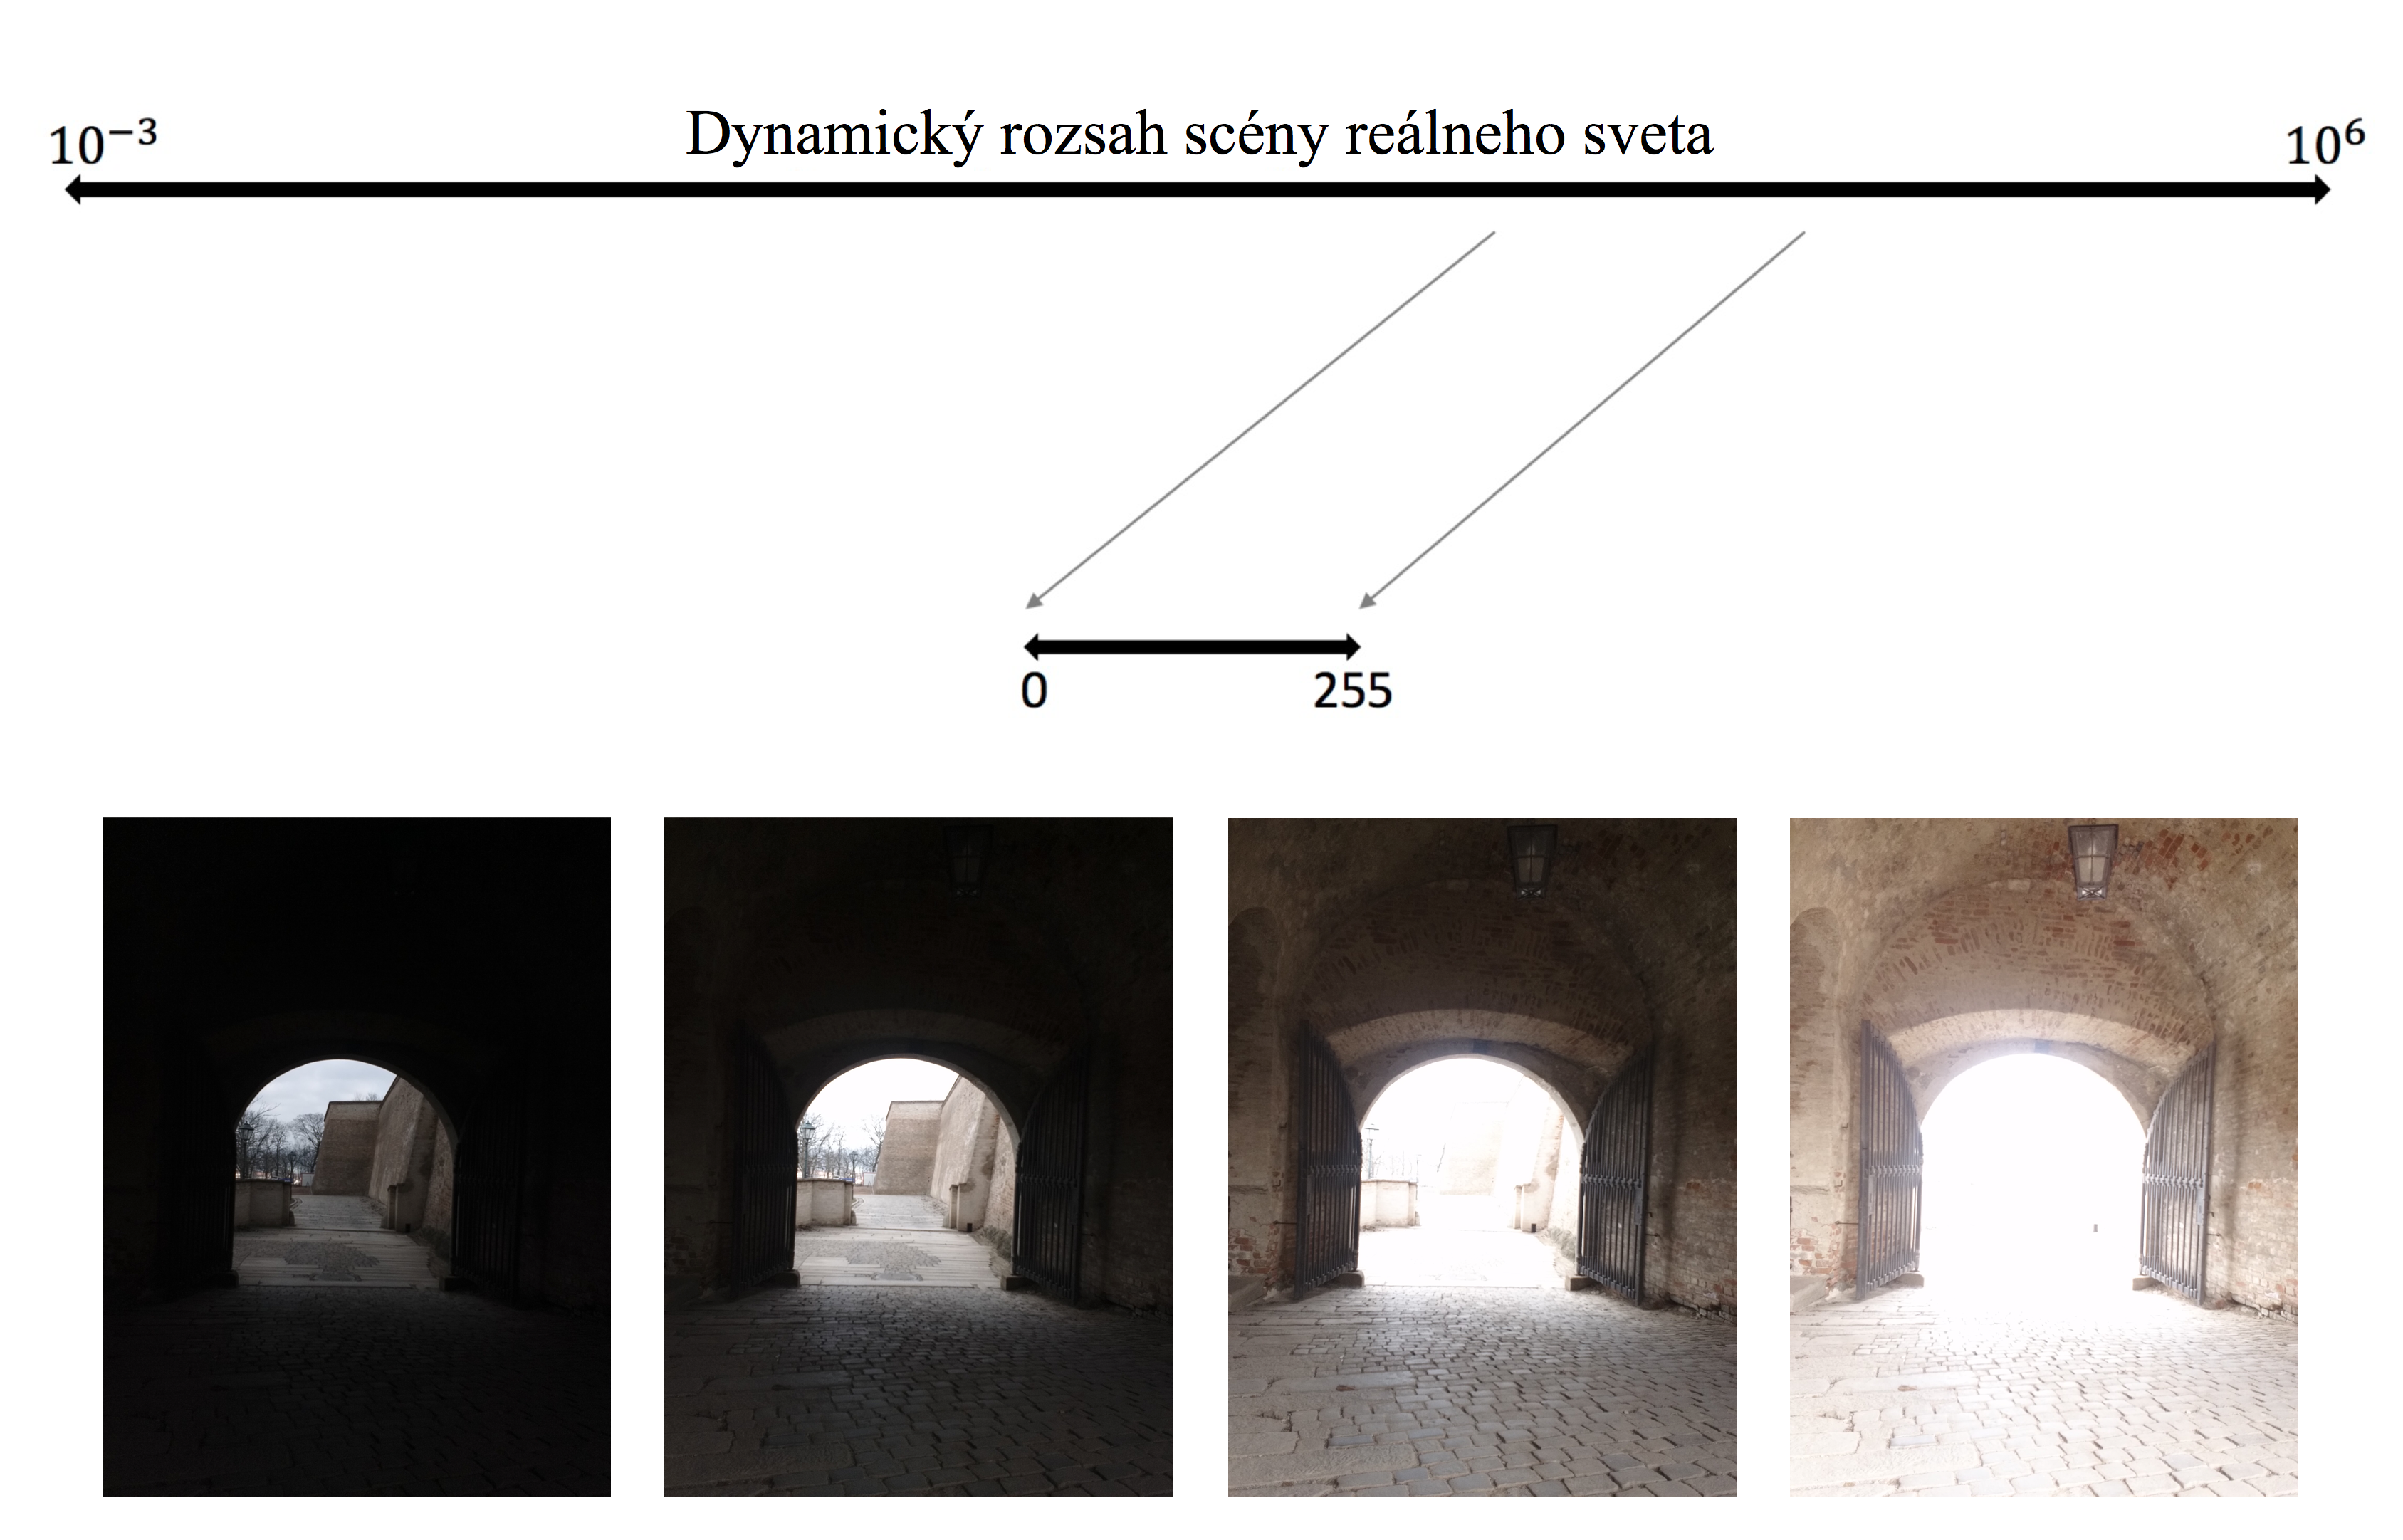
\includegraphics[width=\textwidth]{figures/capturing/capturing_series}
    \caption{Scéna zachytená snímkami s rôznymi hodnotami expozičného času}
    \label{fig:expo_series}
\end{figure}

\subsection{Parametre snímača}

Pred vytváraním fotografie s manuálnymi nastaveniami parametrov snímača je dobré poznať základné pojmy
\cite{ZakladyHDR}\cite{AHDR}:
\begin{description}
    \item [Expozícia] udáva celkové množstvo svetla dopadajúce na fotografické médium. Je závislá na čase expozície,
    clone a citlivosti ISO. Fotografia s nedostatočným množstvom svetla je podexponovaná a naopak fotografia s príliš
    veľkým množstvom svetla je preexponovaná.
    \item [Expozičný čas] udáva dobu, počas ktorej je svetlocitlivý snímač vystavený dopadajúcemu svetlu. Čím je hodnota
    expozičného času vyššia, tým viac svetla sa prepustí fo vnútra fotoaparátu a tým je snímka svetlejšia. Expozičný čas
    sa udáva v sekúndách, prípadne v zlomkoch sekundy (8, 4, 2, 1, 1/2, 1/4...).
    \item [Clona] vytvára otvor v objektíve, cez ktorý prechádza svetlo z vonkajšieho prostredia na~svetlocitlivý snímač
    fotoaparátu. Čím je clonové číslo nižšie, tým viac svetla sa prepúšťa do vnútra fotoaparátu. Clona ovplyvňuje
    expozíciu, hĺbku ostrosti a kresbu objektívu.
    \item [Citlivosť ISO] určuje mieru citlivosti snímača na dopadajúce svetlo. S rastúcou citlivosťou rastie miera šumu,
    ktorý sa prejavuje ako náhodne farebné pixely vo fotografii. Šum je zretelnejší hlavne v tmavých oblastiach a prejavuje
    sa tiež pri dlhších expozíciách vplyvom zahrievania snímača.
    \item [Hodnota expozície] (EV) je číslo, ktoré predstavuje kombináciu expozičného času a clonového čísla. Táto hodnota udáva
    určité množstvo zachyteného svetla zo scény pri pevne danej hodnote citlivosti ISO (obvykle ISO100). Pri kombinácii času
    expozície $t$ a clonového čísla $N$ je EV definované ako:
    $EV = \ln_{2}\frac{N^{2}}{t}$.
    \item [Snímač] fotoaparátu, alebo snímací čip, je umiestnený za objektívom a tvorí najdôležitejší prvok fotoaparátu.
    Dôležitými vlastnosťami snímačov fotoaparátu sú jeho rozmer (čím väčší rozmer, tým kvalitnejší výsledný obraz) a počet
    pixelov, z ktorých sa snímač skladá.

    Snímače sa podľa technológie výroby delia na CCD\footnote{Charge–Coupled Device} a CMOS\footnote{Complementary Metal Oxide Semiconductor}.
    Oba typy snímačov obsahujú maticu pixelov (senzorov), ktoré sú zložené zo subpixelov, vo väčšine prípadov usporiadaných do tzv.
    Bayerovej masky. Každý subpixel má priradený farebný filter, ktorý sa používa na filtrovanie dopadajúceho svetla a tým môže zaznamenať
    iba jednu farebnú zložku. Ak však na tento subpixel dopadne fotón, ktorého vlnová dĺžka reprezentuje inú farbu, akú je filter
    schopný prepustiť, stráca sa farebná informácia. CMOS čipy sú najpoužívanejším typom senzorov. Ich výroba je konštrukčne náročnejšia,
    ale majú nižšiu spotrebu energie a rýchlejší prenos dát. Dáta prenášajú z~každého bodu samostatne, zatiaľ čo CCD po celých riadkoch.
\end{description}

\subsection*{Rozdiel medzi LDR a HDR snímkami}

Hlavný rozdiel medzi LDR\footnote{low dynamic range} snímkami a snímkami HDR je v hodnotách pixelov.
Hodnoty pixelov v HDR sú vo všeobecnosti spájané s jasom. Pixely nevyjadrujú presné hodnoty
jasu, pretože fotoaparát má inú spektrálnu citlivosť ako ľudské oko, ale iba aproximujú 
fotometrické veličiny. Približná odchýlka od fotometrických meraní je v rozsahu od 10\% 
pre achromatické (šedé) povrchy až po 30\% pre farebné objekty \cite{DCmerania}.

\section{Generovanie HDR}
\label{sec:Theory-Generating}

V úvode vysvetlíme význam premenných, ktoré budú použité nielen pri zápise rovníc, ale aj v zdrojovom
kóde aplikácie:
\begin{itemize}
    \item $P$ - počet obrázkov s rozličnou expozíciou,
    \item $N$ - počet pixelov v jednom obrázku,
    \item $Z_{ij}$ - hodnota pixelu, kde $i$ je index pixelu a $j$ index obrázku,
    \item $Z_{min}$, $Z_{max}$ - hodnota minima a maxima, ktorú môže pixel nadobudnúť,
    \item $\Delta t_{j}$ - expozičný čas pre $Z_{ij}$,
    \item $w(Z_{ij})$ - váhová funkcia odstraňujúca presahujúce hodnoty.
\end{itemize}

Ak by mal fotoaprát lineárnu odozvu, intenzita žiarenia $E$ pre pixel na indexe $i$ by mohla byť 
vytvorená kombináciou hodnôt, zaznamenaných pre každú expozíciu a pre každý farebný kanál ako
\begin{equation}
    E_{i} = \frac{
            \sum_{j=1}^{P}
            \frac{1}{\Delta t_{j}}
            w(Z_{ij})Z_{ij}
        }{
            \sum_{j=1}^{P}
            w(Z_{ij})
        }
    \cite{AHDR}
\end{equation}

Avšak digitálne fotoaparáty nemajú lineárnu odozvu, ale všeobecnú funkciu nazývanú krivka odozvy
fotoaparátu (CRF\footnote{Camera Response Function}). Predtým, ako sa bude generovať HDR obsah,
je potrebné vyjadriť túto krivku odozvy. Na to slúži algoritmus od Paul E. Debeveca a Jitendra Malika, 
založený na využívaní fyzikálnej vlastnosti zobrazovacích systémov, ktorú nazveme reciprocita.
Reciprocita vyjadruje reakciu svetlocitlivého materiálu ako inverzný vzťah medzi intenzitou svetla 
a času osvetlenia. Pri štandardnom rozsahu expozície je odozva fotoaparátu určená celkovou expozíciou 
definovanou ako intenzita $\times$ čas. \cite{AHDR}

\subsection{Získanie krivky odozvy fotoaparátu} 

Vstupom algoritmu sú fotografie vytvorené s rôznou dĺžkou času expozície $\Delta t_{j}$. Za predpokladu, 
že hodnoty intenzity žiarenia $E_{i}$ pre každý pixel $i$ sú konštanty, môžeme zapísať rovnicu 
reciprocity ako:
\begin{equation} \label{eq:reciprocity}
    Z_{ij} = f(E_{i} \Delta t_{j})
    \cite{Debevec}
\end{equation}
Keďže je funkcia $f$ monotónna, potom je aj invertovateľná a rovnicu \ref{eq:reciprocity} môžeme
zapísať ako $f^{-1}(Z_{ij}) = E_{i} \Delta t_{j}$. Pridaním prirodzeného logaritmu na obe strany 
získame \\$\ln f^{-1}(Z_{ij}) = \ln E_{i} + \ln \Delta t_{j}$. Následne si definujeme funkciu
$g = \ln f^{-1}$ a dostaneme súbor rovníc:
\begin{equation} \label{eq:gFunction}
    g(Z_{ij}) = \ln E_{i} + \ln \Delta t_{j}
    \cite{Debevec}
\end{equation}

Cieľom algoritmu je pomocou metódy najmenších štvorcov vyjadriť funkciu krivky odozvy $g$ a intenzitu
žiarenia $E_{i}$, ktoré najlepšie vyhovujú súboru rovníc \ref{eq:gFunction}. Keďže rozsah hodnôt jasu
je konečný, vyjadrujeme iba konečný počet hodnôt krivky odozvy $g$. Vyjadrením celočíselných hodnôt
pixelov $Z_{min}$ a $Z_{max}$, počtu polôh pixelu $N$ a počtu fotografií $P$, definujeme problém ako
hľadanie $(Z_{max} - Z_{min})$ hodnôt pre $g(Z)$ a $N$ hodnôt pre $\ln E_{i}$, ktoré minimalizujú
kvadratickú objektívnu funkciu:
\begin{equation} \label{eq:objFunction}
    \mathcal{O} = 
    \sum_{i=1}^{N}
    \sum_{j=1}^{P}
    [g(Z_{ij}) - \ln E_{i} - \ln \Delta t_{j}]^{2}
    + \lambda
    \sum_{z=Z_{min} + 1}^{Z_{max} - 1}
    g''(z)^{2}
    \cite{Debevec}
\end{equation}
Prvý term zabezpečuje, že riešenie vyhovuje súboru rovníc vyplývajúcich z rovnice \ref{eq:gFunction}
a~druhý term zabezpečuje plynulosť funkcie $g$. Hodnota $\lambda$ je váha plynulosti, relatívna 
k~prvému termu a je zvolená podľa množstva šumu očakávaného v $Z_{ij}$.

\begin{figure}[t]
    \centering
    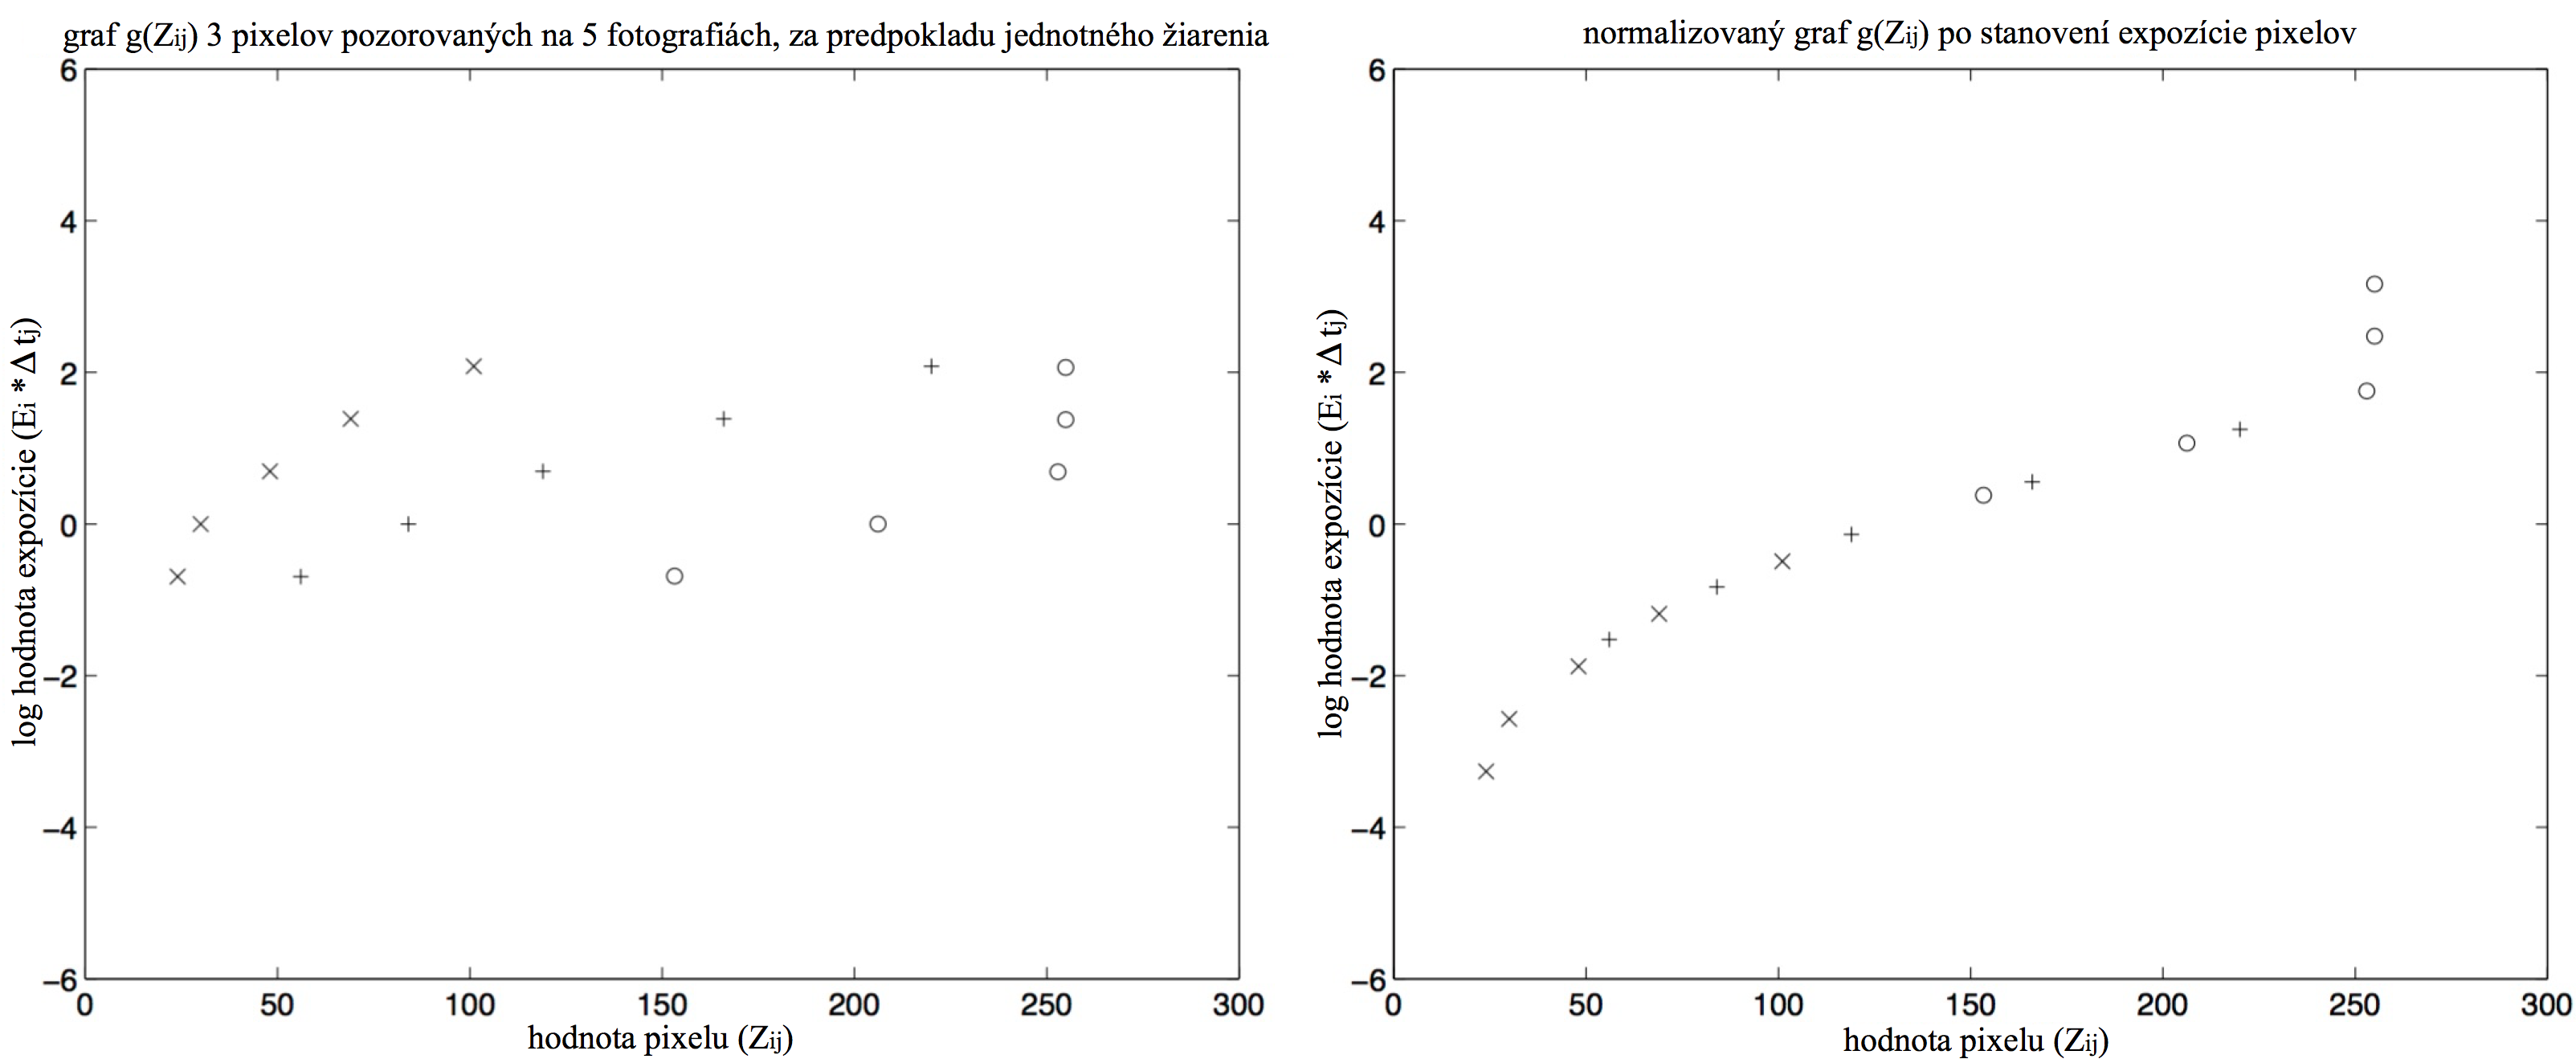
\includegraphics[width=\textwidth]{figures/generating/normalized-curve}
    \caption{Normalizácia hodnôt $Z_{ij}$ riešením rovnice \ref{eq:objFunction} \cite{Debevec}}
\end{figure}

\section{Zobrazovanie HDR}
\label{sec:Theory-Displaying}

HDR fotografie by mali verne vizuálne reprezentovať scénu, na ktorej sa na nachádzajú. Hlavným problémom
je, že úroveň intenzity jasu HDR fotografie môže prekročiť výstupnú úroveň reprodukovanú výstupným médiom
(obr. \ref{fig:luminance_range}). Rovnako aj kontrast môže presiahnúť rozsah kontrastu zobrazovateľný médiom.
Táto skutočnosť platí ako pre tlač, tak aj pre zobrazovacie zariadenia.

Vzhľad scény závisí od úrovne osvetlenia a rozsahu kontrastu\cite{HDRI}. Za jasného dňa vyzerá scéna viac
farebne a kontrastnejšie. Pre reprodukovanie presného vizuálneho vzhľadu takejto scény nestačí iba jednoduchá
kompresia, aby sa úroveň intenzity a rozsah kontrastu prispôsobil limitom zobrazovacieho média.

Reprodukcia vizuálneho vzhľadu je primárnym cieľom pre mapovanie tónov. Aktuálne je otvoreným problémom
výskumov definovanie a číselné vyjadrenie vizuálneho vzhľadu scény. Tieto výskumy zároveň podporujú vývoj
farebných modelov.

\begin{figure}[t]
    \centering
    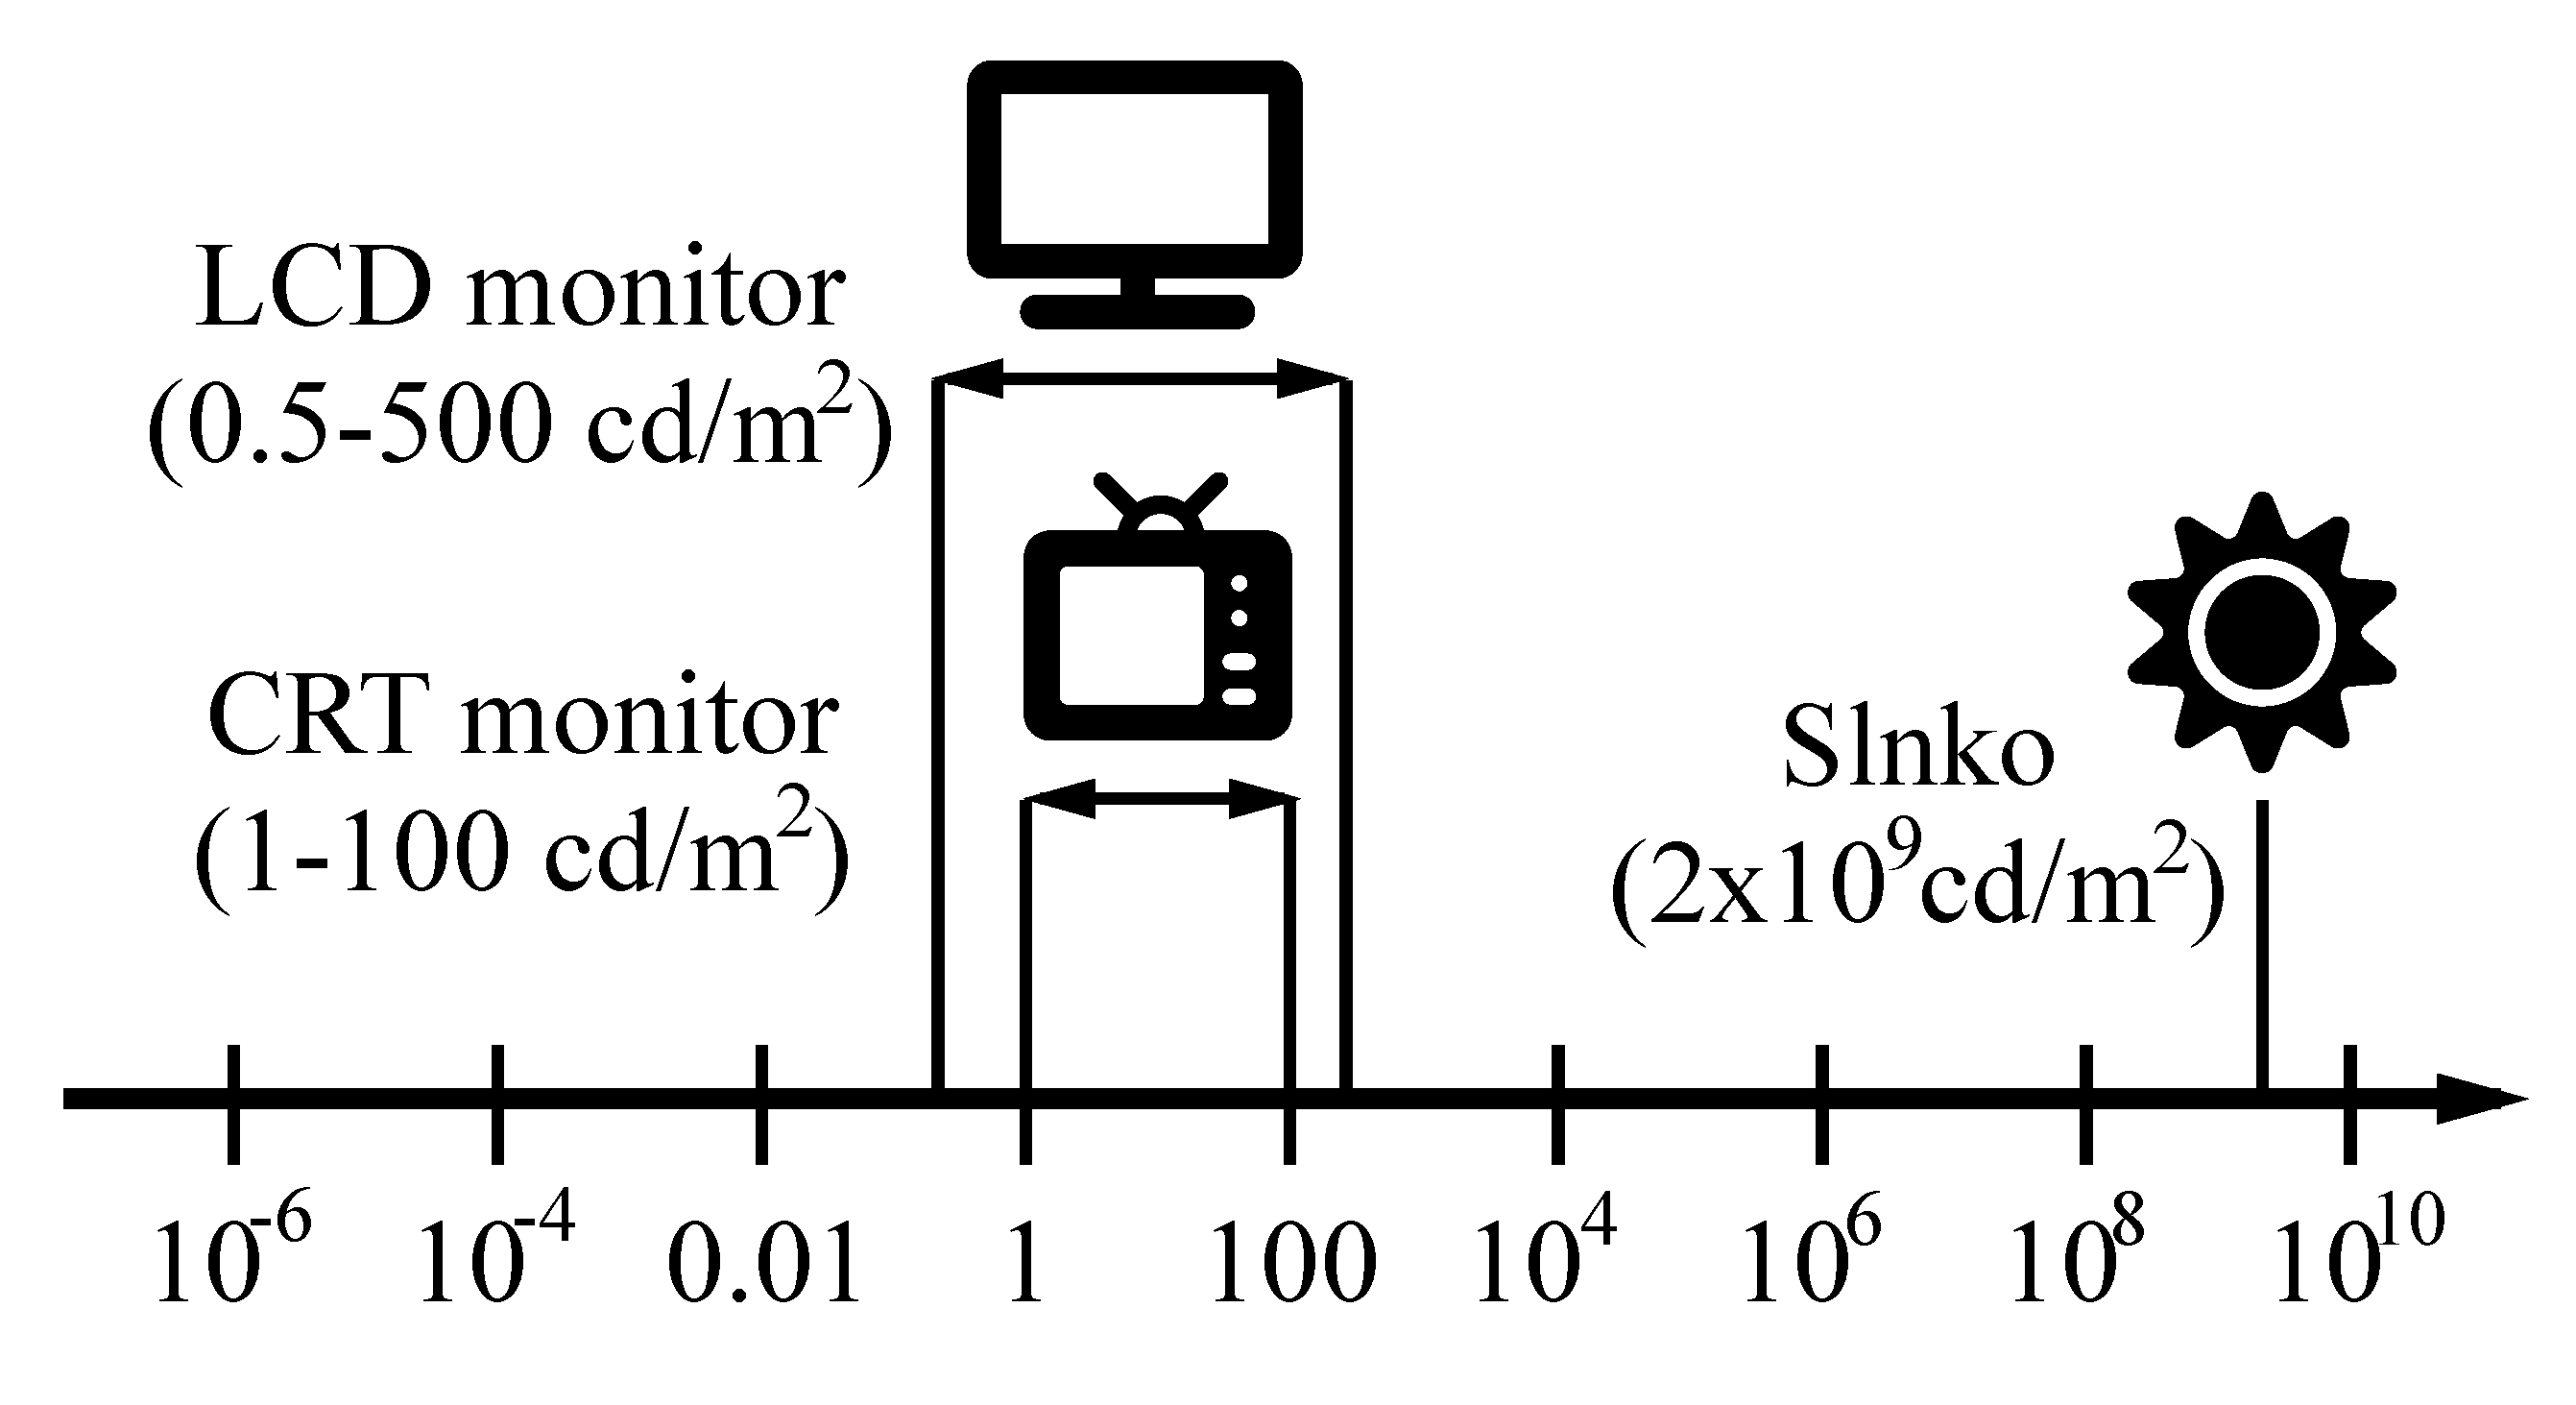
\includegraphics[width=0.6\textwidth]{figures/tonemap/monitor_range}
    \caption{Hodnoty jasu reálneho sveta v porovnaní s rozsahom jasu, 
    ktorý možno zobrazovať na LCD a CRT monitoroch \cite{Mantiuk}}
    \label{fig:luminance_range}
\end{figure}

\subsection*{Mapovanie tónov}

Mapovanie tónov je proces prevodu obrazu s vysokým dynamickým rozsahom na 8-bitový obraz pre farebný kanál, 
s cieľom zachovať čo najväčší počet detailov. Mapovanie tónov znižuje dynamický rozsah alebo kontrastný pomer
celého záberu so zachovaním lokálneho kontrastu. \cite{AHDR}

Existuje viacero metód mapovania tónov a ich ciele môžu byť rozličné v závislosti od konkrétneho využitia.
V niektorých prípadoch je hlavným cieľom vytvárať len esteticky príjemné obrázky, zatiaľ čo iné metódy
reprodukujú čo najväčší počet obrazových detailov alebo maximalizujú kontrast obrazu. Cieľom vykresľovacích 
aplikácií môže byť dosiahnutie čo najväčšej zhody medzi skutočnou scénou a zobrazeným obrázkom, aj keď
zobrazovacie zariadenie nedokáže reprodukovať celý rozsah hodnôt jasu.

\subsection{Operátory mapovania tónov}
\label{sec:Theory-Operators}

Väčšina metód mapovania tónov sa zameriava na susediace pixely a s ich informáciami môže vykonať tónovanie,
napríklad nastavením jasu vo vzťahu k susediacím pixelom. Jedným zo spôsobov je rozostriť oblasť, čo spriemeruje
jas a potom túto informáciu použiť. \cite{ZakladyHDR} Rozostrenie sa neaplikuje na obrázok, iba sa využije
k výpočtom.

V posledných rokoch boli vyvinuté rôzne metódy mapovania tónov, ktoré je môžeme rozdeliť do dvoch základných
typov:
\begin{description}
    \item [Globálne operátory] (priestorovo jednotné) sú nelineárne funkcie založené na svetelných a iných
    globálnych premenných obrazu. Akonáhle je optimálna funkcia odhadnutá podľa konkrétnej snímky, každý pixel
    v obraze je mapovaný rovnakým spôsobom, nezávisle od hodnoty okolitých pixelov v obraze. Tieto techniky 
    sú jednoduché a~rýchle, ale môžu spôsobiť stratu lokálneho kontrastu.
    \cite{AHDR}
    
    \item [Lokálne operátory] (priestorovo sa meniace) sú nelineárnej funkcie, ktorých parametre sa menia
    v každom pixeli podľa vlastností získaných z okolitých oblastí. Inými slovami, efekt metódy sa mení
    pre každý pixel podľa vlastností obrazu na danom mieste. Tieto metódy sú zložitejšie ako globálne
    a môžu vytvárať artefakty, ako napríklad halo efekt alebo kontrastné obrysy a tým môže výstup metódy vyzerať
    nerealisticky. Avšak poskytujú lepší výsledok, pretože ľudské vnímanie je citlivé hlavne na lokálny kontrast.
    \cite{AHDR}
\end{description}

Medzi najznámejšie metódy mapovania tónov patria:
\begin{description}
    \item [Bilaterálny filter]
    (Durand a Dorsey 2002) - lokálny operátor, ktorý zachováva detaily. Metóda sa pokúša zobraziť obrazy HDR
    rozložením obrazu na základnú vrstvu a~vrstvu detailov. V základnej vrstve je kontrast skomprimovaný
    bilaterálnym filtrom, ktorý chráni hrany. \cite{TMODurand}

    \item [Fotografická reprodukcia]
    (Reinhard a spol. 2002) - tento operátor simuluje techniku "dodging and burning", ktorá bola používaná
    v počiatkoch fotografie a dovoľuje vytvárať rozličné expozície naprieč fotografiou. Lokálny operátor
    obsahuje aj jednoduchšiu globálnu verziu. \cite{TMOReinhard}
    
    \item [Logaritmické mapovanie]
    (Drago a spol. 2003) - metóda redukuje pomer kontrastu logaritmickou kompresiou hodnôt jasu,
    napodobňujúc ľudské vnímanie svetla. Zachováva detaily a kontrast scény. \cite{TMODrago}

    \item [Perceptuálny rámec pre kontrastné spracovanie HDR]
    (Mantiuk a spol.) - metóda vytvára rámec pre spracovanie obrazu v priestore vizuálnej odozvy, v ktorej
    kontrastné hodnoty priamo korelujú so svojou viditeľnosťou v obraze. Rámec zahŕňa transformáciu obrazu
    z jasového priestoru na pyramídu obrázkov s nízkym kontrastom a potom do priestoru vizuálnej
    odozvy. \cite{TMOMantiuk}

    \item [Kompresia gradiendom]
    (Fattal a spol.) - metóda znižuje rozsah gradiendového poľa jasu. Obraz s nízkym dynamickým rozsahom
    je získaný riešením Poissonovej rovnice na modifikovanom gradiendovom poli. Metóda je schopná dobrej
    kompresie dynamického rozsahu, pričom zachováva jemné detaily a vyhýba sa bežným artefaktom. \cite{TMOFattal}

    \item [Úprava histogramu] (Larson a spol. 1997) - cieľom operátora je vytvárať HDR fotografie, ktoré
    zachovávajú realistickosť scény. Obsahuje modely citlivosti človeka na kontrast, farby, ostrosť zraku
    a osvetlenie, podľa ktorých sa vytvárajú obrazy zodpovedajúce skúsenostiam diváka na skutočnej scéne.
    \cite{AHDR}

    \item [Model iCAM]
    (Johnson a Fairchild 2003) - model vzhľadu obrazu, ktorý bol rozšírený pre zobrazovanie HDR obrázkov
    na displej. iCAM sa pokúša určiť perceptuálnu odozvu voči priestorovo zložitým podnetom a dokáže predvídať
    vzhľad HDR obrazu. \cite{TMOFairchild}
    
    \item [Lokálny model prispôsobenia očí]
    (Ledda a spol. 2004) - simuluje reakciu sietnice na~jas, avšak v tomto prípade je proces úplne lokalizovaný,
    čo umožňuje dobrú kompresiu dynamického rozsahu. Tento model je podobný modelu Pattanaika a spol. z roku 2000.
    \cite{TMOLedda}
\end{description}

\section{Formáty HDR obsahu} \label{section-formats}

Po vygenerovaní HDR obsahu, sa môže vyžadovať jeho uloženie pre neskoršie úpravy a~spracovanie. Vygenerovaný HDR obsah
s hodnotami v desatinných číslach s pohyblivou rádovou čiarkou, zaberá 96 bitov pre pixel. Na uloženie takého obsahu,
je vhodné obsah komprimovať do jedného zo zavedených formátov, uvedených v tabuľke \ref{table:formats}.
Veľa schém na komprimovanie HDR obsahu je založených na existujúcich štandardoch komprimovania LDR obrázkov.
Cieľom kompresie HDR obrazu je reprezentácia hodnôt s pohyblivou rádovou čiarkou menším počtom bitov.

\begin{table}[h!]
\centering
\begin{tabular}{||c|c|c||} 
  \hline
  Formát & Kódovanie & Bity/pixel \\
  \hline\hline
  \multirow{2}{4em}{HDR} 
  & RGBE & 32 \\ 
  & XYZE & 32 \\
  \hline
  \multirow{3}{4em}{TIFF} 
  & IEEE RGB & 96 \\
  & LogLuv24 & 24 \\
  & LogLuv32 & 32 \\
  \hline
  \multirow{1}{4em}{EXR} 
  & Half RGB & 48 \\
  \hline
\end{tabular}
\caption{Zavedené formáty HDR obsahu \cite{HDRI}}
\label{table:formats}
\end{table}

\subsection*{RGBE}

Formát Radiance HDR (\texttt{.hdr}, \texttt{.pic}), je jeden z prvých formátov pre komprimovanie HDR obsahu. 
Súbor zakódovaný v tomto formáte je zložený z hlavičky so základnými informáciami o parametroch obrázku a komprimovaných 
dát. Pixel uložený vo formáte RGBE má 32 bitov (obr. \ref{fig:rgbe}). Prvých 24 bitov obsahuje jednotlivé farebné kanály v štandardnej
forme hodnôt 0-255 (8 bitov). Posledných 8 bitov je vyhradených pre spoločný exponent. S~ohľadom na to, 
že hodnoty RGB sú vo veľmi podobnom rozsahu, nie je potrebné ukladať exponent zvlášť pre každý farebný kanál.
Exponent je vyjadrený z najjasnejšieho kanálu.

Obmedzením formátu RGBE je, že nemôže reprezentovať vysoko saturované farby v~rámci farebného modelu sRGB. Pri konvertovaní
takýchto farieb sa môže stať, že sa farebné zložky stanú zápornými. V takom prípade RGBE nemôže reprezentovať záporné hodnoty
a niektoré informácie o farbe sa stratia. Riešením tohoto problému je využitie farebného modelu CIE XYZ a kódovanie XYZE. \cite{AHDR}

\begin{figure}[h!]
  \centering
  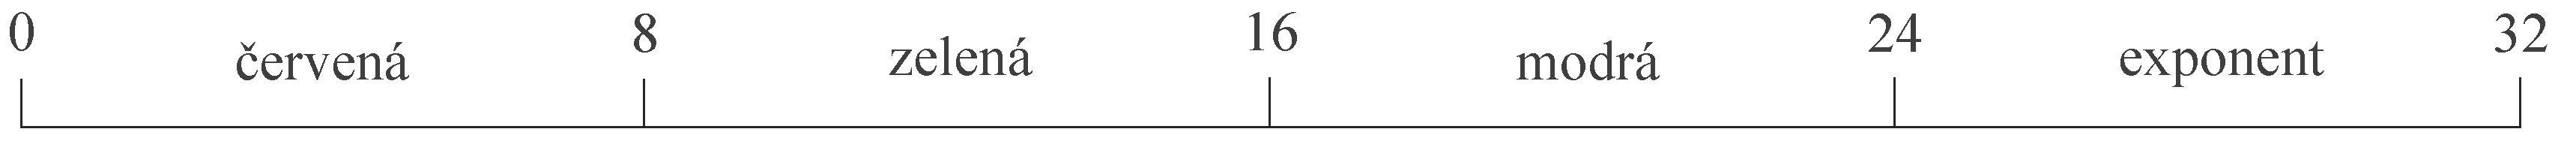
\includegraphics[width=1\textwidth]{figures/storage/rgbe}
  \caption{Formát RGBE, s kódovaním 32 bitov pre pixel}
  \label{fig:rgbe}
\end{figure}

\subsection*{LogLuv}

Kódovanie LogLuv (\texttt{.tif}, \texttt{tiff}), používa na vyjadrenie celého rozsahu jasu a farieb iba celé čísla. Kódovanie
je založené na jave, že ľudské oko nie je rovnako citlivé na všetky úrovne jasu. Ak sa namiesto jasu použije jeho logaritmus,
potom nezáleží na detekovateľných hodnotách prahu, ale konštantné celočíselné hodnoty môžu byť prijateľné pre aproximáciu 
prahu viditeľnosti ľudského oka. \cite{HDRI}

32-bitové kódovanie využíva 16 bitov pre hodnoty jasu a ďalších 16 bitov na reprezentáciu chrominancie (obr. \ref{fig:logluv}).

\begin{figure}[h!]
  \centering
  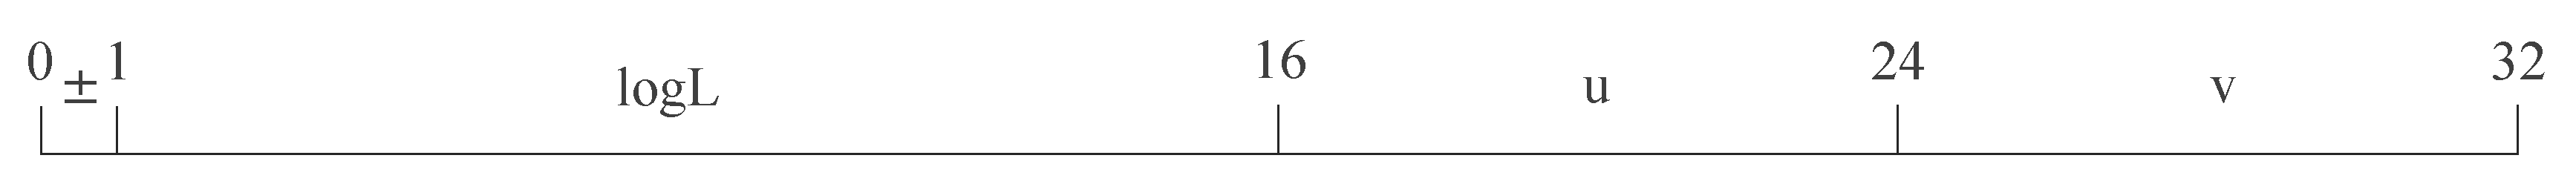
\includegraphics[width=1\textwidth]{figures/storage/logluv}
  \caption{Formát LogLuv, s kódovaním 32 bitov pre pixel}
  \label{fig:logluv}
\end{figure}

\subsection*{OpenEXR}

EXtended Range formát\footnote{\url{http://www.openexr.org}} (\texttt{.exr}) implementovaný v C++ je od roku 2002 dostupný ako open source.
Odvtedy sa stal štandardom pre mnoho aplikácií s HDR obsahom a neustále sa rozvíja aj vo filmovom priemysle. Hodnoty pixelov ukladá
ako 16 alebo 32-bitové číslo s pohyblivou rádovou čiarkou alebo 32-bitové celé číslo. Základná verzia, ktorá využíva 16~bitov
pre farebný kanál, obsahuje 1 znamienkový bit, 5 bitov pre exponent a 10 bitov pre mantisu (obr. \ref{fig:exr}). Formát podporuje
bezstrátovú kompresiu a rozšíriteľnosť knižnice o vlastnú funkcionalitu. \cite{HDRI}

\begin{figure}[h!]
  \centering
  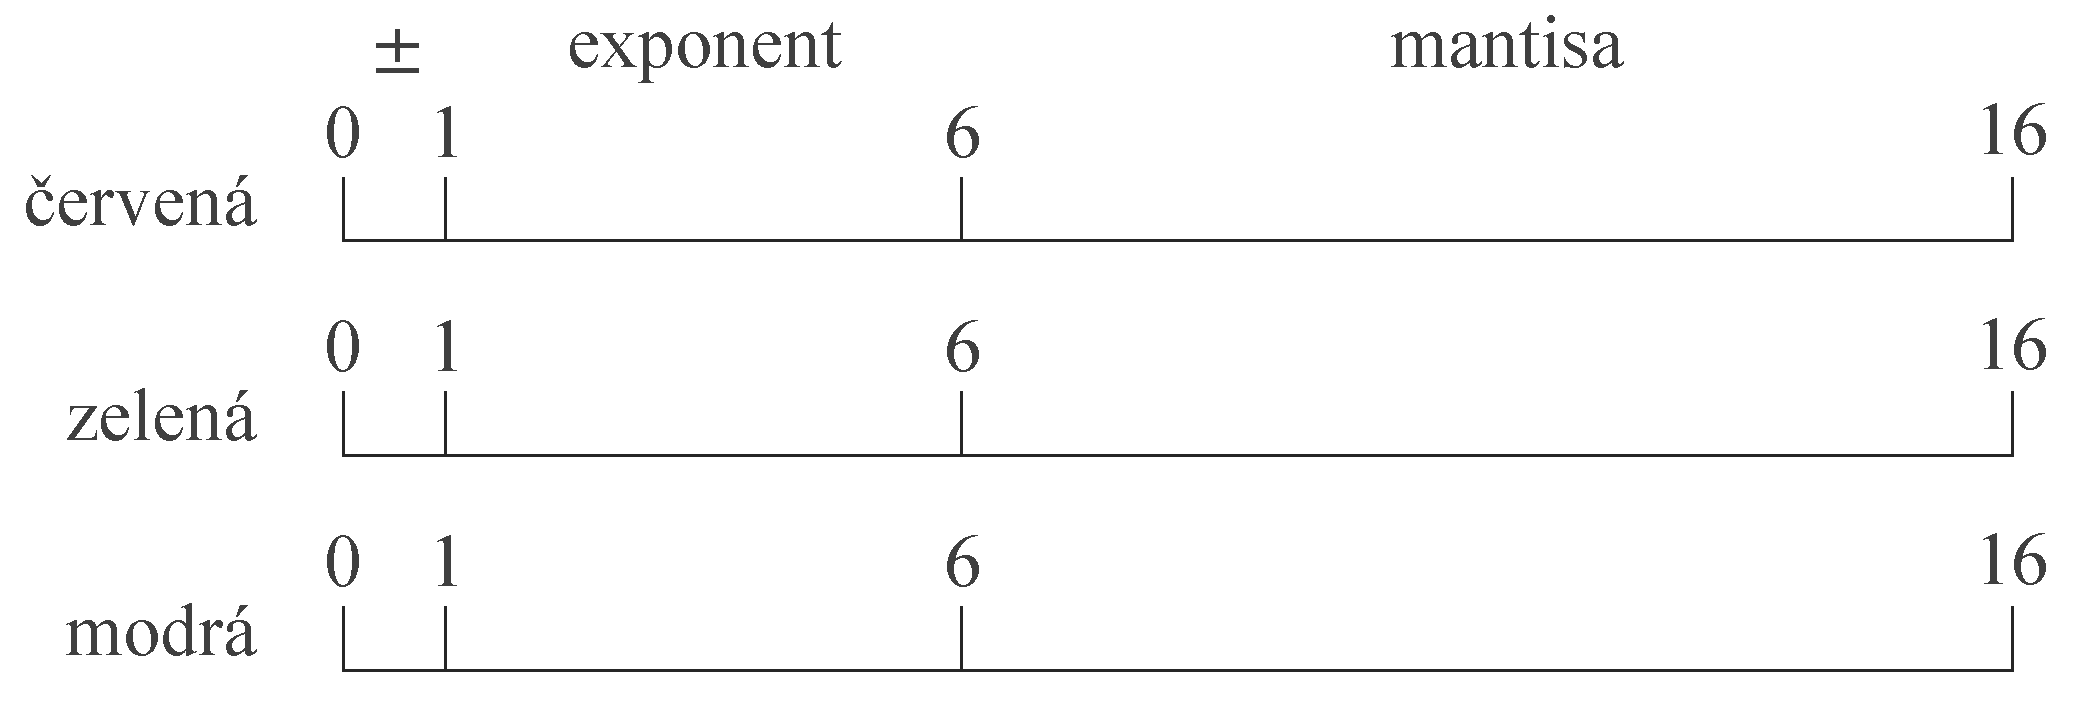
\includegraphics[width=0.6\textwidth]{figures/storage/exr}
  \caption{Formát OpenEXR, s kódovaním 48 bitov pre pixel}
  \label{fig:exr}
\end{figure}

\chapter{Existujúce riešenia}
Pre vytvorenie aplikácie, ktorá bude spĺňať požiadavky širokej škály užívateľov
a bude obsahovať prakticky využiteľné funkcie je potrebné spraviť prieskum existujúcich riešení
rovnako zameraných aplikácií dostupných na GooglePlay (pre Android) a iTunes (iOS).
Nižšie je uvedený zoznam najsťahovanejších mobilných aplikácií pre jednotlivé OS, ich funkcie, výhody,
nevýhody a chyby z užívateľského hľadiska.

\subsection*{Android}

\begin{description}
    \item [HDR Max - Photo Editor] (hodnotenie užívateľov 4.3/5)
    Na vytvorenie fotografie využíva natívnu aplikáciu Fotoaparát. Pri jednom spustení sa to ukázalo ako
    nevhodný spôsob, keďže sa po vytvorení fotografie neotvorila znova aplikácia. HDR fotografiu vytvára 
    pomocou filtra aplikovaného na jednu fotografiu. Filter sa dá dokonca kombináciou s inými krokmi naniesť 
    viac krát, čo sa dá považovať za chybu. Upravovanie HDR je veľmi obmedzené. Aplikácia obsahuje štandardné 
    úpravy vytvorenej fotografie (kontrast, jas, sýtosť, teplota a vyváženie farieb) a statické farebné filtre
    (obr. \ref{fig:appsUI_1}). Okrem toho má aplikácia ešte širokú ponuku, niekedy zbytočných funkcií.

    \item [Ultimate HDR Camera] (4.11/5)
    Fotografia sa vytvára v rozhraní aplikácie. Pre vytvorenie HDR formátu využíva kombináciu viacero vytvorených
    fotografií s rôzným expozičným časom. Následne vytvorená HDR fotografia má obmedzené úpravy. Aplikácia je
    veľmi jednoduchá, ale užívateľa nezaujme svojím rozhraním (obr. \ref{fig:appsUI_2}). Napriek tomu, výsledné snímky
    sú kvalitné zobrazenia scény s akýmkoľvek dynamickým rozsahom.

    \item [Snapseed] (4.5/5)
    Vytvorenie fotografie nie je možné, aplikácia dokáže iba načítať uloženú fotografiu z galérie, na ktorú je
    možné aplikovať filter, ktorý vytvára HDR efekt. Aplikácia však zaujala svojou ponukou grafických nástrojov,
    z ktorých najzaujímavejšie sú napr. nastavenie kriviek, perspektívy, retro filtre, rozpoznávanie tváre
    a efekt zostrenia (obr. \ref{fig:appsUI_3}). Aplikácia taktiež ponúka niekoľko málo farebných filtrov. Roz-hranie
    je intuitívne, a veľmi dobre premyslené vzhľadom na komplikované nástroje a možnosti úprav. Nastavovanie intenzity
    jednotlivých filtrov a úprav je zaujímavo implementované - pre výber nástroja využíva potiahnutie prstom vertikálne
    a potiahnutím prstom do strán nastavujeme intenzitu úpravy. Z pohľadu užívateľa je to najzaujímavejšia aplikácia
    na GooglePlay.

    \item [HDR Camera] (3.8/5)
    Fotografia sa vytvára v rozhraní aplikácie. Aplikácia vytvorí tri fotografie s rôznou expozíciou, čo trvá
    približne 5 sekúnd. Aplikácia je jedna z mála, ktorá nepoužíva na vytvorenie HDR filter. Po vytvorení HDR
    fotografie, nemá užívateľ žiadne ďalšie možnosti úprav. Užívateľ musí dostatočne rýchlo uložiť svoju výslednú
    fotografiu, pretože aplikácia sa svojvoľne prepína naspäť na domovskú obrazovku.

    \item [HDR HQ] (3.9/5)
    HDR fotografiu vytvára pomocou filtra aplikovaného na jednu vytvorenú fotografiu. Obsahuje obmedzené úpravy
    vytvorenej fotografie (kontrast, jas, teplota farieb). Užívateľa však zaujme jednoduché a minimalistické
    rozhranie aplikácie (obr. \ref{fig:appsUI_4}). Dôležitý nedostatok je však chýbajúce tlačidlo pre návrat
    z obrazovky úprav do hlavného menu.

    \item [A Better Camera] (4.1/5)
    Aplikácia obsahuje rôzne možnosti fotografovania scény, medzi ktorými je aj možnosť vytvorenia HDR fotografie.
    HDR fotografiu vytvára pomocou troch fotografií s rôznou expozíciou a výsledok je pre užívateľa dostatočne uspokojivý.
    Vytvorenú fotografiu je možne upravovať pomocou externej aplikácie od rovnakého vývojára.

\end{description}

\subsection*{iOS}

\begin{description}
    \item [HDR]
    HDR efekt vytvára pomocou jedného z piatich filtrov a nastavením jeho intenzity. Rozhranie je jednoduché
    a pre užívateľa nezaujímavé.

    \item [HDR Camera]
    Aplikácia je totožná s Android aplikáciou HDR HQ, čo pridáva pozitívnu vlastnosť - multiplatformnosť.
    Obdobne teda ako HDR HQ na Androide má veľmi zaujímave grafické rozhranie a zaujímavú ponuku úprav fotografie.

    \item [HDR for Free]
    Vytvorenie fotografie nie je možné, aplikácia dokáže iba načítať uloženú fotografiu z galérie, na ktorú je
    možné aplikovať jeden zo štyroch filtrov vytvárajúcich HDR efekt. Výsledok je aj tak veľmi neuspokojivý - iba
    sa zvýši kontrast farieb. Grafické rozhranie aplikácie je veľmi chabé.

    \item [Live HDR Camera]
    Fotografia sa vytvára v rozhraní aplikácie, kde užívateľ môže v reál-nom čase sledovať výsledok pomocou filtra
    obrazu. Obraz však obsahuje množstvo šumu a po vytvorení fotografie užívateľ dostane fotografiu upravenú filtrom
    s množstvom šumu. Po vytvorení fotografie aplikácia neponúka žiadne ďalšie nastavenia a~úpravy fotografie.

    \item [Snapseed]
    Aplikácia obsahuje všetky možnosti úprav a nástrojov ako Android aplikácia Snapseed.

    \item [Adobe Lightroom]
    Fotografia sa vytvára v rozhraní aplikácie, kde užívateľ môže nastavovať EV. HDR fotografiu následne vytvorí pomocou
    filtra. Užívateľovi ponúka štandardné úpravy a nastavenia, avšak rozhranie je veľmi ťažkopádne a neprehľadné.

\end{description}

\begin{figure}[t]
    \centering
    \begin{subfigure}{0.4\textwidth}
        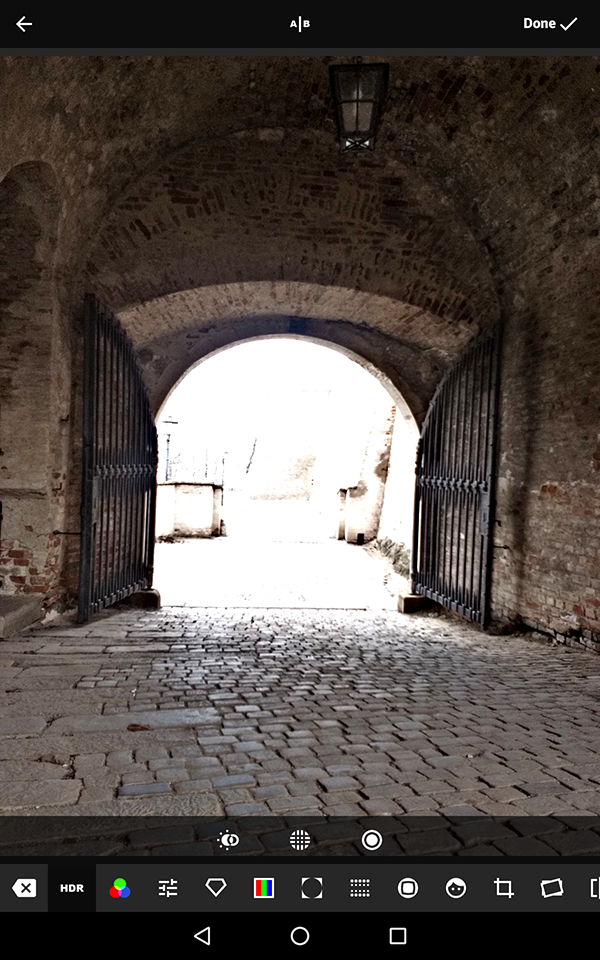
\includegraphics[width=\textwidth]{figures/ui/apps/uiHdrMax}
        \caption{HDR Max}
        \label{fig:appsUI_3}
    \end{subfigure}
    ~
    \begin{subfigure}{0.4\textwidth}
        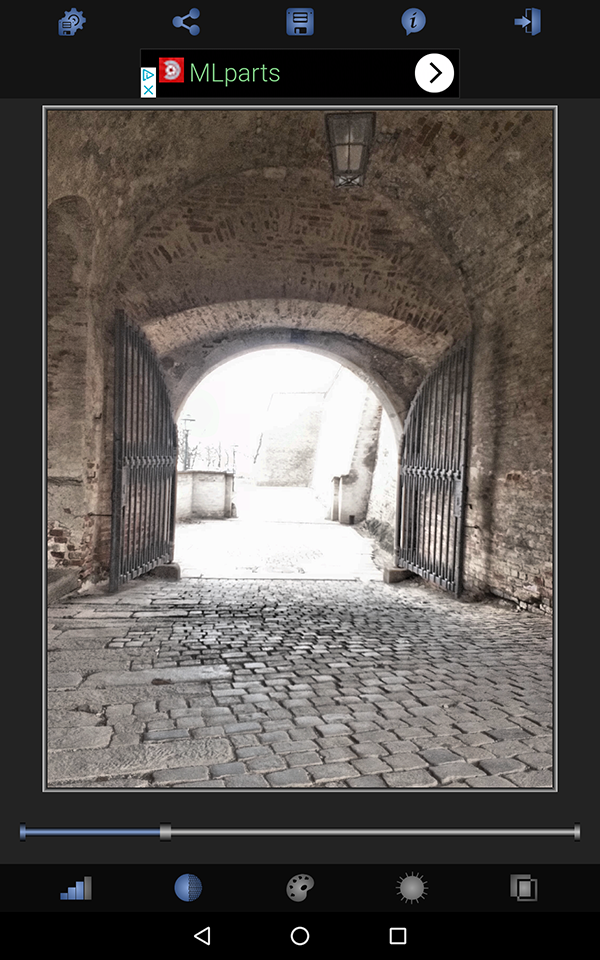
\includegraphics[width=\textwidth]{figures/ui/apps/uiUltimateHdr}
        \caption{Ultimate HDR Camera}
        \label{fig:appsUI_4}
    \end{subfigure}

    \begin{subfigure}{0.4\textwidth}
        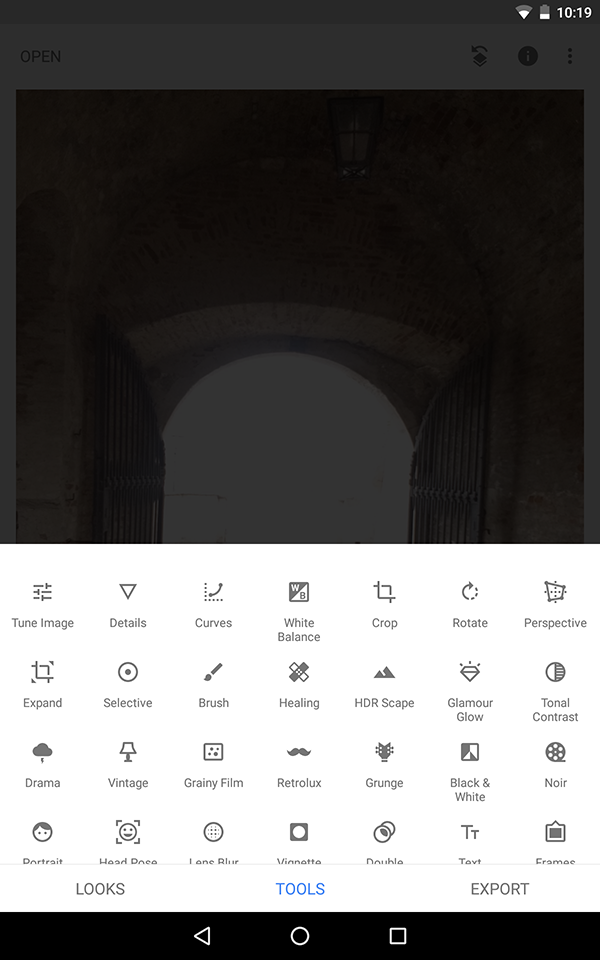
\includegraphics[width=\textwidth]{figures/ui/apps/uiSnapseed}
        \caption{Snapseed}
        \label{fig:appsUI_1}
    \end{subfigure}
    ~
    \begin{subfigure}{0.4\textwidth}
        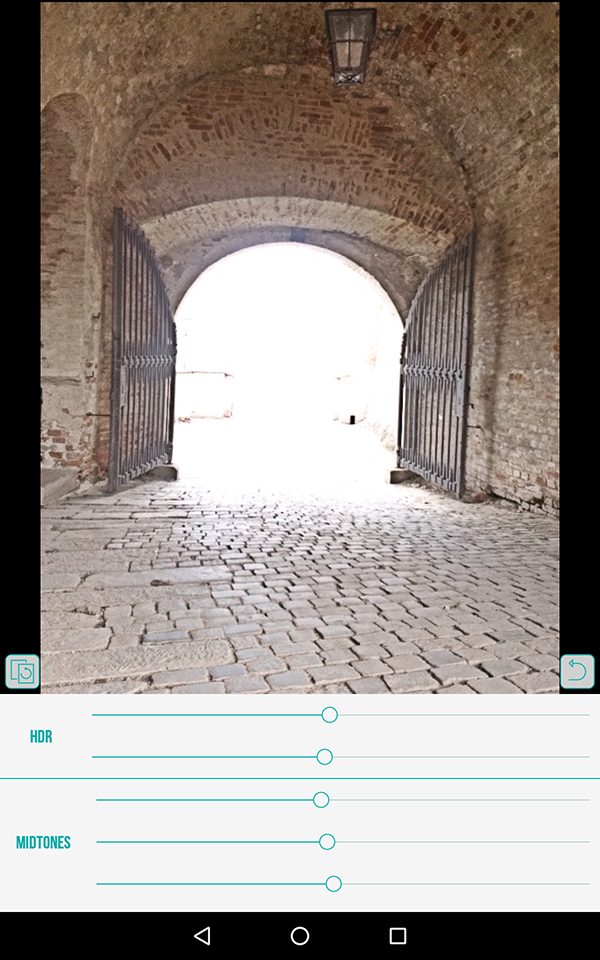
\includegraphics[width=\textwidth]{figures/ui/apps/uiHdrHq}
        \caption{HDR HQ}
        \label{fig:appsUI_2}
    \end{subfigure}
    \caption{Užívateľské rozhrania podobných aplikácií}
    \label{fig:appsUI}
  \end{figure}

\chapter{Návrh a implementácia}
Výber technológií pre implementáciu časovo a priestorovo náročných algoritmov je dôležitá a často 
náročná časť práce. Vzhľadom k tomu, že natívna aplikácia fotoaparátu pre iOS podporuje vytváranie
HDR fotografie, táto práca bude zameraná na platformu Android. Použité vývojové prostredie je
Android Studio, ktoré poskytuje širokú škálu nástrojov pre editovanie kódu a zároveň ponúka tvorbu 
viziálneho návrhu grafického užívateľského rozhrania. Zvoleným programovacím jazykom je objektovo 
orientovaná Java. Pre riešenie náročných matematických a grafických operácií je použitá knižnica
OpenCV. Knižnica je implementovaná v jazyku C++, čo znamená, že metódy sú v operačnom systéme Android
vykonávané natívne a tým nám prináša výhodu v rýchlosti spracovania.

Aplikácia implementuje štandardný postup vytvárania HDR fotografie na základe spájania série snímok
(obr. \ref{fig:app_pipeline}). Užívateľské rozhranie aplikácie poskytuje užívateľovi možnosti
interaktivity pri vytváraní výslednej fotografie. Pre zarovnanie snímok je použitá metóda Median
Threshold Bitmap od Grega Warda (viac v podkapitole \ref{sec:Practice-Alignment}). 
Využitím krivky odozvy zariadenia, ktorú dosiahneme metódou od Paula E. Debeveca a Jitendru Malika,
popísanou v podkapitole \ref{sec:Theory-Generating} a váhovej funkcie, vygenerujeme HDR obsah,
ktorý je sám o~sebe nezobraziteľný. Vygenerovaný HDR obsah možno zobraziť pomocou operátorov mapovania
tónov. Aplikácia implementuje celkovo štyri operátory mapovania tónov: globálny operátor Erika Reinharda,
operátor Frederika Draga a lokálne operátory od Duranda a~Mantiuka (podkapitola \ref{sec:Theory-Operators}).

Zdrojový kód aplikácie je členený podľa architektonického vzoru model-view-controller, ktorý rozdeľuje
aplikáciu do troch hlavných častí:
\begin{description}
  \item [Dátový model] uchováva dáta naprieč aplikáciou a operácie nad týmito dátami.
\end{description}
\setlength{\DTbaselineskip}{2em}
\dirtree{%
.1 model.
.2 CameraCRF \DTcomment{Krivka odozvy zariadenia}.
.2 Exposures \DTcomment{Vybrané expozičné časy pre aktuálnu scénu}.
.2 ImageHDR \DTcomment{HDR obsah}.
.2 ImageLDR \DTcomment{Vytvorená fotografia}.
.2 TmoParams \DTcomment{Východzie hodnoty a prevod relatívnych hodnôt na absolútne}.
}

\begin{description}
  \item [Užívateľské rozhranie] umožňuje prezentáciu dát. V našom prípade \texttt{view} obsahuje
  triedy pracujúce s Android Fragmentmi (viac v podkapitole \ref{sec:Practice-UI}) a dialógovými oknami.
\end{description}
\setlength{\DTbaselineskip}{2em}
\dirtree{%
.1 view.
.2 CameraFragment.
.2 EditDragoFragment.
.2 EditDurandFragment.
.2 EditMantiukFragment.
.2 EditReinhardFragment.
.2 FilesFragment.
.2 HomeFragment.
.2 SaveDialog.
.2 SettingsDialog.
.2 TmoFragment.
}

\begin{description}
  \item [Riadiaca logika aplikácie] riadi tok udalostí v programe a modifikuje dáta v dátovom modeli.
\end{description}
\setlength{\DTbaselineskip}{2em}
\dirtree{%
.1 controller.
.2 camera.
.3 AlignImages \DTcomment{Zarovnanie série fotografií}.
.2 hdr.
.3 CRFRecover \DTcomment{Získanie krivky odozvy zariadenia}.
.3 HDRController \DTcomment{Kontrolér postupu vytvárania HDR obsahu}.
.3 HDRMerge \DTcomment{Generovanie HDR obsahu}.
.3 SamplesSelector \DTcomment{Výber vzorky pixelov}.
.2 tmo \DTcomment{Metódy operátov mapovania tónov}.
.3 TMODrago.
.3 TMODurand.
.3 TMOMantiuk.
.3 TMOReinhard.
.2 Convertor \DTcomment{Prevody medzi dátovými typmi}.
.2 Storages \DTcomment{Správa úložísk zariadenia}.
}

\begin{figure}[t]
  \centering
  \includegraphics[width=1\textwidth]{figures/ui/pipeline}
  \caption{Postup vytvárania HDR fotografie pomocou aplikácie}
  \label{fig:app_pipeline}
\end{figure}
\section{Užívateľské rozhranie}
\label{sec:Practice-UI}

Aplikácia sa zameriava na širokú škálu užívateľov - od náročného fotografa až po technicky neskúsenú
osobu, snažiacu sa vytvoriť čo najdôveryhodnejší záber scény. Preto by mala aplikácia minimalistickým 
a intuitívnym spôsobom ponúkať všetky potrebné nástroje a~možnosti, ktoré môže užívateľ využiť.

\begin{figure}[h!]
  \centering
  \begin{subfigure}{0.3\textwidth}
      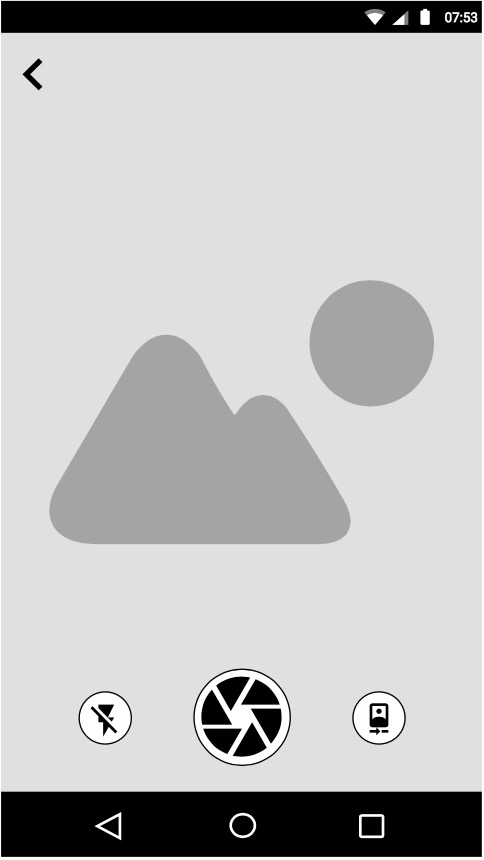
\includegraphics[width=\textwidth]{figures/ui/sketches/sketch-capture}
      \caption{Snímanie fotografie}
      \label{fig:sketch_capture}
  \end{subfigure}
  ~
  \begin{subfigure}{0.3\textwidth}
      
\includegraphics[width=\textwidth]{figures/ui/sketches/sketch-home}
      \caption{Domovská obrazovka}
      \label{fig:sketch_home}
  \end{subfigure}
  ~
  \begin{subfigure}{0.3\textwidth}
      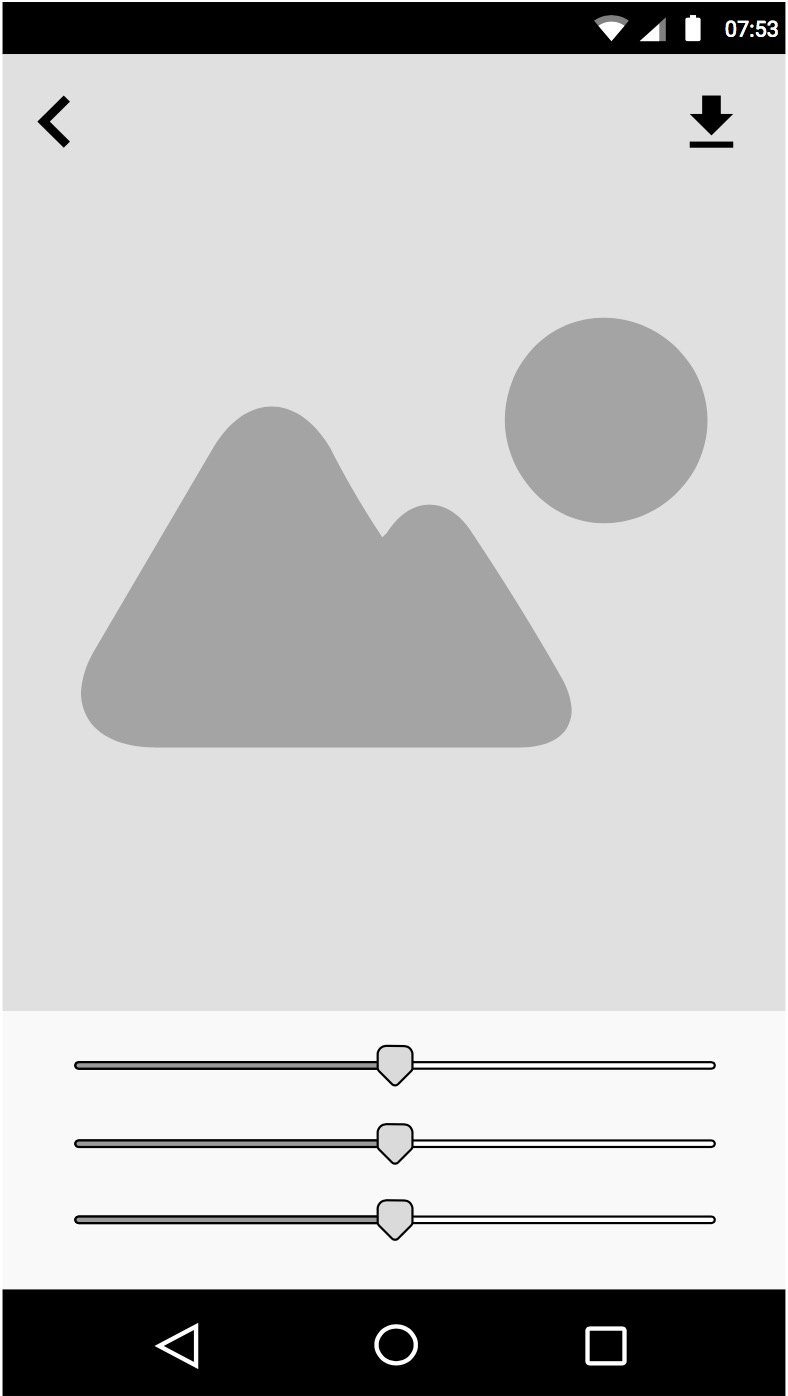
\includegraphics[width=\textwidth]{figures/ui/sketches/sketch-edit}
      \caption{Úprava fotografie}
      \label{fig:sketch_edit}
  \end{subfigure}
  \caption{Návrh obrazoviek užívateľského rozhrania}
  \label{fig:sketch_screens}
\end{figure}

Obrazovka \ref{fig:sketch_home} je príkladom toho, že užívateľ môže mať všetko čo potrebuje,
bez zbytočného zdĺhavého hľadania. Na vytvorenie HDR fotografie potrebujeme buď zachytiť aktuálnu scénu
fotoaparátom, alebo načítať súbor s HDR obsahom.

Po zachytení scény na fotografiu (obr. \ref{fig:sketch_capture}) alebo načítaní HDR obsahu a po spracovaní 
tohoto obsahu, má užívateľ na výber z rôznych techník mapovania tónov. Po výbere jednej z nich je
užívateľovi poskytnutá možnosť upravovania fotografie (obr. \ref{fig:sketch_edit}) do výslednej podoby 
pomocou prehľadnej ponuky nástrojov. Jednotlivé parametre sú spočiatku nastavené na vhodné východzie 
hodnoty, ktoré je možné po úpravach zresetovať. Na záver je možné výsledok uložiť do galérie. Rozhranie 
musí ponúkať aj možnosť vrátiť sa o obrazovku späť, na čo aplikácie z prieskumu existujúcich riešení 
často zabúdajú.

Náhľadová ikona (obr. \ref{fig:appIcon}) je navrhnutá, aby zachytila hlavnú myšlienku aplikácie.
Tri vrstvy s rozdielnými odtieňmi od najtmavšieho po najsvetlejší predstavujú fotografie zachytené
s rôznym časom expozície. Ich prelínanie naznačuje, že sa tieto snímky spájajú do jednej HDR fotografie.
Pôvodný čierno-biely návrh ikony časom nahradila varianta v~primárnych farbách užívateľského rozhrania.

\begin{figure}[h!]
    \centering
    
\includegraphics[width=0.3\textwidth]{figures/ui/logo/logo_bw}
    
\includegraphics[width=0.3\textwidth]{figures/ui/logo/logo}
    \caption{Ikona aplikácie}
    \label{fig:appIcon}
\end{figure}

Z domovskej obrazovky (obr. \ref{fig:homeScreen_hints}) je priamy prístup k nastaveniam aplikácie (obr.
\ref{fig:homeScreen_settings}). Nastavenia obsahujú možnosti definovania počtu vytvorených fotografií
v jednej sérii a zvolenie kroku pre algoritmus vyberajúci vhodné časy expozície (podkapitola
\ref{sec:Practice-ExpoSelector}).

\begin{figure}[h!]
    \centering
    \begin{subfigure}{0.35\textwidth}
        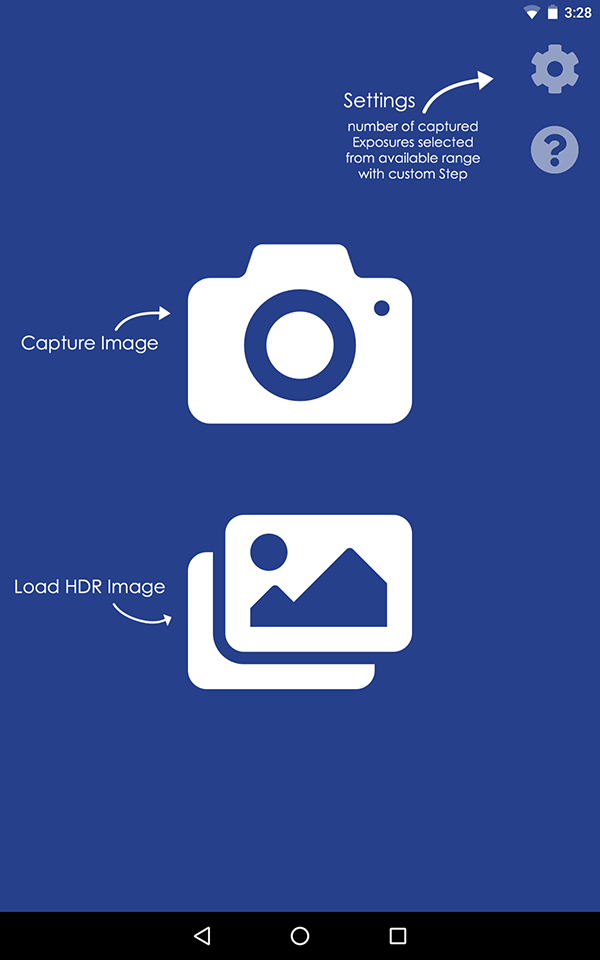
\includegraphics[width=\textwidth]{figures/ui/home/screenHome}
        \caption{Popis obrazovky}
        \label{fig:homeScreen_hints}
    \end{subfigure}
    ~
    \begin{subfigure}{0.35\textwidth}
        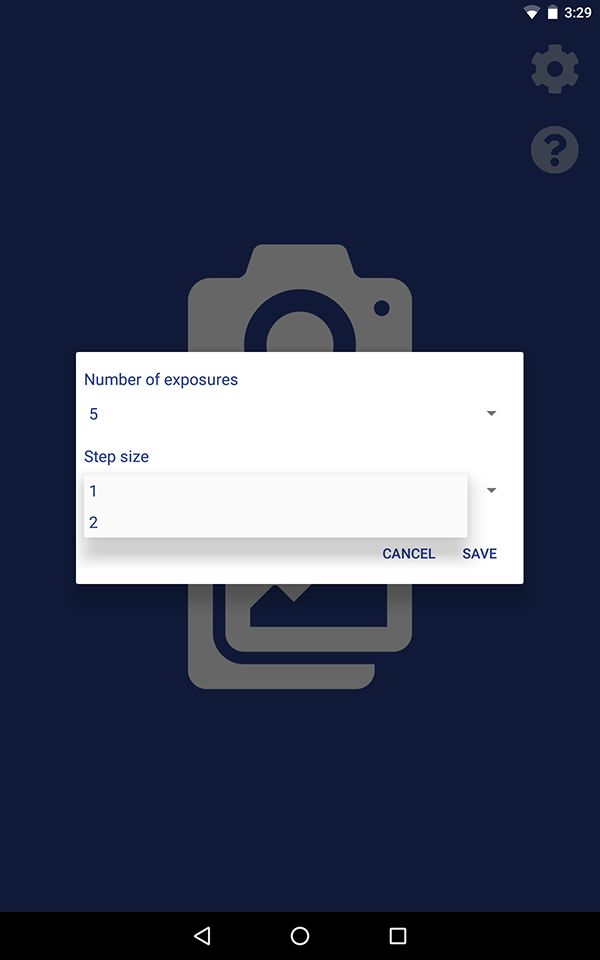
\includegraphics[width=\textwidth]{figures/ui/home/dialogSettings}
        \caption{Nastavenia aplikácie}
        \label{fig:homeScreen_settings}
    \end{subfigure}
    \caption{Domovská obrazovka}
    \label{fig:homeScreen}
\end{figure}

\subsection*{Android Fragment}

\begin{figure}[h!]
    \centering
    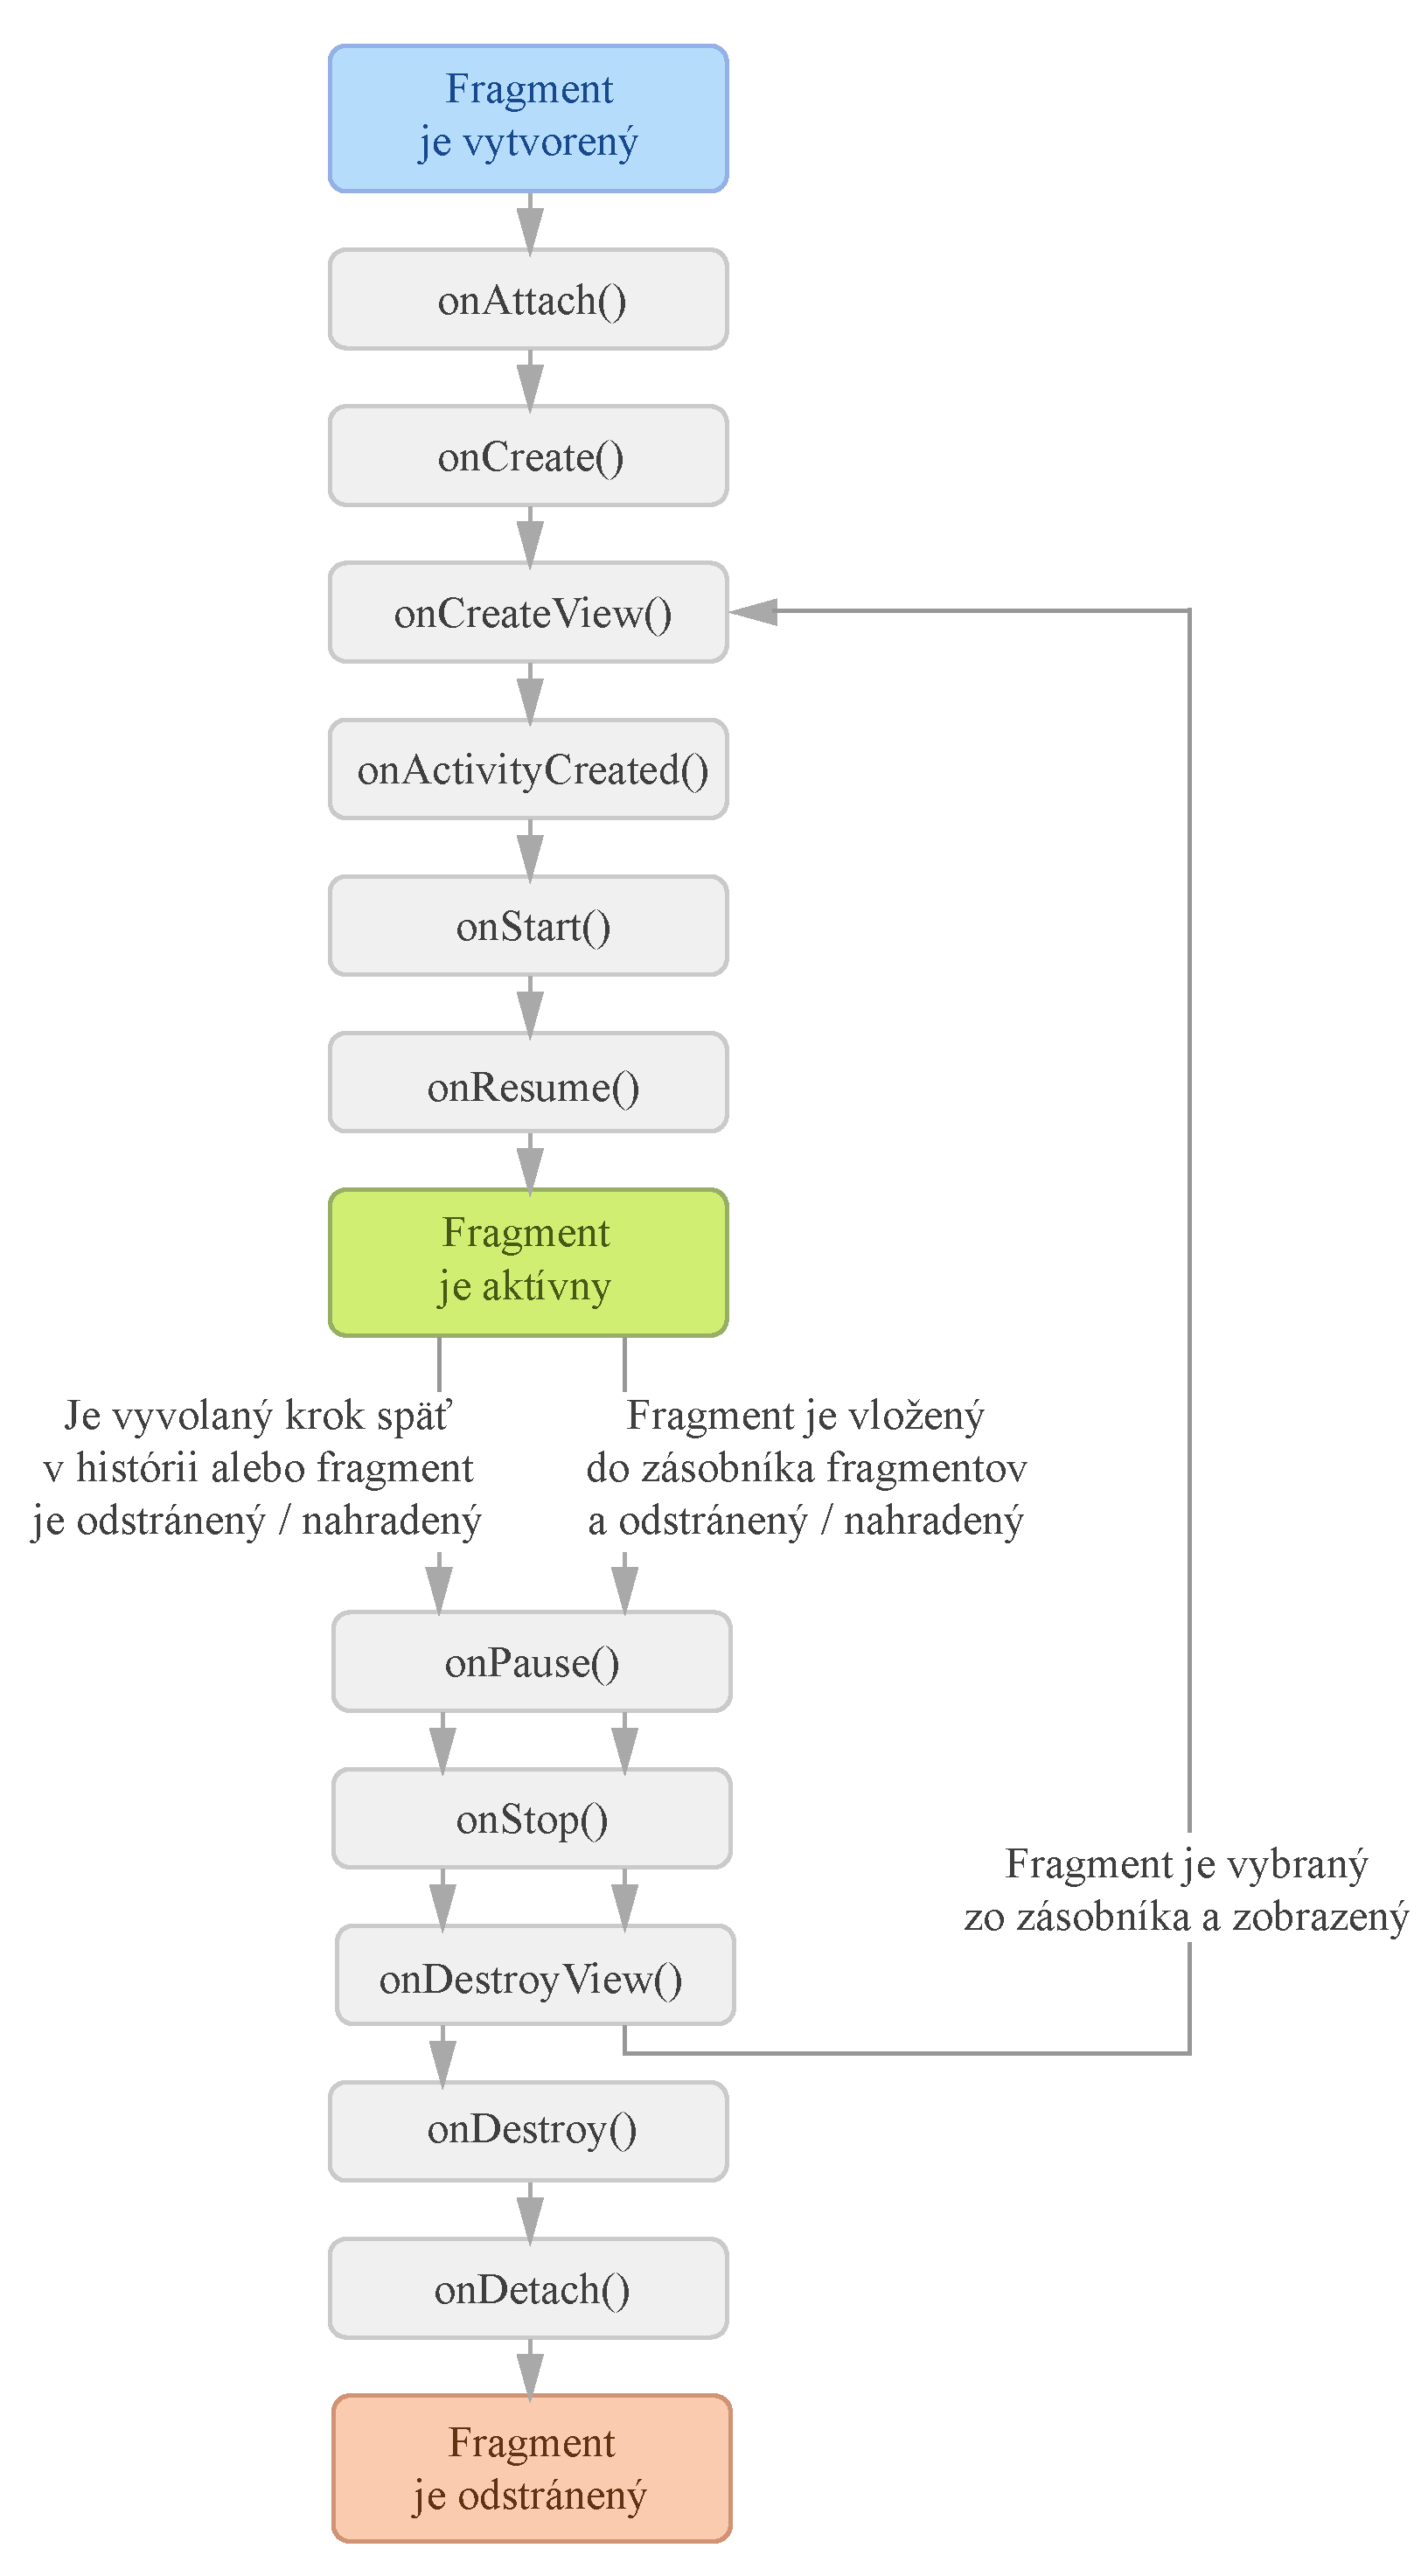
\includegraphics[width=0.5\textwidth]{figures/ui/fragment_lifecycle}
    \caption{Životný cyklus Fragmentu \cite{Android}}
    \label{fig:fragment_lifecycle}
\end{figure}

Jednotlivé obrazovky aplikácie sú vytvorené využitím Android Fragmentov. \texttt{Fragment} popisuje vymedzenú
časť užívateľského rozhrania, ktorú je možné vkladať, alebo odoberať počas behu aktivity. 
V hlavnej obrazovke aktivity je definovaný \texttt{FrameLayout} \texttt{container}, do ktorého sa podľa
situácie vkladajú obrazovky typu Fragment.

V triede \texttt{Main} aplikácie vkladáme jednotlivé obrazovky pomocou \texttt{FragmentTransaction} transakcií,
ku ktorým vytvára prístup \texttt{FragmentManager}.

\begin{lstlisting}[morekeywords={ExampleFragment,FragmentManager,FragmentTransaction,R}]
ExampleFragment newFragment = new ExampleFragment();

FragmentManager manager = getSupportFragmentManager();
FragmentTransaction transaction = manager.beginTransaction();

transaction.replace(R.id.fragment_container, newFragment);
transaction.addToBackStack(null);
transaction.commit();
\end{lstlisting}

Zásobník \texttt{BackStack} slúži na pohybovanie sa v histórii fragmentov aplikácie. To znamená, že ak užívateľ klikne
na tlačidlo späť, zo zásobníka sa vyberie posledný aktívny fragment a zobrazí sa. Typ našej aplikácie tento zásobník
nevyžaduje. Tlačidlá späť slúžia primárne na vrátenie sa na domovskú obrazovku, prípadne na obrazovku s výberom
operátora mapovania tónov.

Vykreslenie obrazovky v rozhraní zabezpečuje objekt \texttt{LayoutInflater}. Prvky a rozloženie obrazovky
je definované v jazyku XML.
\begin{lstlisting}[morekeywords={View, LayoutInflater, ViewGroup, Bundle}]
public View onCreateView(LayoutInflater inflater, ViewGroup container, Bundle savedInstanceState) {
    return inflater.inflate(R.layout.new_fragment, container, false)
}                                  
\end{lstlisting}

\section{Snímanie}
\label{sec:Practice-Capturing}

Aplikácia generuje HDR obsah kombinovaním LDR fotografií s rôznou hodnotou času expozície.
Snímanie fotografií je implementované nad aplikačým rozhraním
Camera2\footnote{\url{https://developer.android.com/reference/android/hardware/camera2/package-summary.html}}
operačného systému Android. Aplikácii, pracujúcej s týmto rozhraním, musí byť užívateľom udelené povolenie 
\texttt{android.permission.CAMERA}.

Po inicializovaní obrazovky (obr. \ref{fig:sketch_capture}) sa vytvorí inštancia \texttt{CameraManager}, ktorá poskytuje
detekciu, charakterizáciu a pripojenie k dostupným \texttt{CameraDevices} \cite{Android}.
Každá z~\texttt{CameraDevices} obsahuje súbor vlastností a nastavení snímača, ku ktorým pristupujeme pomocou
objektu \texttt{CameraCharacteristics}.

Následne je vytvorená \texttt{CameraCaptureSession}, ktorej zvolíme výstupnú oblasť \texttt{Surface}. 
Pre zobrazovanie scény v reálnom čase zobrazujeme na výstup stream záberov scény, ktorý dosiahneme nastavením
opakovaného požiadavku o snímanie. \texttt{CaptureRequest} (požiadavok o~snímanie) vytvárame nastavovaním parametrov
objektu \texttt{CaptureRequest.Builder}. Pri zobrazovaní náhľadu užívateľovi využijeme automatické nastavenia
parametrov snímania (\texttt{CONTROL\_MODE\_AUTO}). Do vytvoreného požiadavku o stream záberov scény vložíme callback
\texttt{CaptureCallback}, ktorého metóda \texttt{onCaptureCompleted} vracia objekt typu \texttt{TotalCaptureResult}.
Tento objekt obsahuje hodnoty konfigurácie snímača zariadenia, po~vytvorení posledného snímku. Z tejto
konfigurácie následne získavame hodnoty času expozície, ISO, clony a korekcie farieb, ktoré sú automaticky zvolené
snímačom. Hodnoty ukladáme do premenných, ktoré neskôr použijeme pri manuálnych nastaveniach snímania. Keďže táto
operácia nie je časovo ani priestorovo náročná a nenarúša plynulé zobrazenie streamu scény a taktiež hodnoty
senzora sa menia vplyvom scény, sú tieto hodnoty nastavované v každom \texttt{CaptureCallback}u po uskutočnení
požiadavku o snímanie.

Ak užívateľ stlačí tlačidlo pre snímanie scény, je zastavené opakovanie požiadavku zobrazovania streamu.
V tomto okamihu je potrebné vytvoriť sériu záberov scény, s manuálne nastavenými hodnotami parametrov.
Dosiahneme to definovaním zoznamu požiadavkov o~snímanie, ktoré budú mať špecifikované hodnoty parametrov.
Pre nastavovanie vlastných parametrov, musí byť aktivovaný manuálny mód a to vypnutím \texttt{CONTROL\_MODE}.
Hodnoty parametrov ako citlivosť snímača (ISO) a clona sú nájdené ako najvhodnejšia kombinácia 
pre najlepší výsledok. Najdôležitejším parametrom je však dĺžka času expozície v nanosekundách,
počas ktorého je snímač vystavený svetlu z prostredia scény.
Zoznam požiadavkov o vytvorenie snímok s manuálnymi parametrami je poslaný do metódy \texttt{captureBurst()}.
Zachytený snímok sa v callbacku \texttt{OnImageAvailableListener} spracuje a vloží do zoznamu k ostatným záberom 
danej scény.

\subsection{Nastavenie času expozície}
\label{sec:Practice-ExpoSelector}

Ako už bolo spomínané, vybrané \texttt{CameraDevice} nám poskytuje vlastnosti snímača, popísané 
v \texttt{CameraCharacteristics} \cite{Android}. Odtiaľ získame aj rozsah povoleného expozičného času snímača 
\texttt{SENSOR\_INFO\_EXPOSURE\_TIME\_RANGE}. Tento rozsah využijeme pri výpočte expozičných časov,
ktoré budú využité pri snímaní. V mnohých zdrojoch sa uvádzajú odporúčané časy expozície vyjadrené ako
hodnoty geometrického radu - každý čas expozície je konštantným násobkom predchadzajúceho času.

Trieda \texttt{Exposures} pomocou postupne získaných informácií o rozsahu povoleného expozičného času snímača
a automaticky zvolenej hodnoty času expozície v aktuálnej scéne vytvára zoznam vybraných expozičných časov pre manuálne
nastavenia. Pri inicializovaní snímača zariadenia a získania rozsahu expozičných časov sú do zoznamu \texttt{range}
postupne vkladané hodnoty času expozície v tvare $2^{n}$ nanosekúnd. V okamihu, keď nastane stav manuálneho snímania scény,
vytvorí sa zoznam vybraných expozičných časov, ktorých strednou hodnotou je hodnota automatickej expozície (obr. \ref{fig:expoSelector0}).
Povolený rozsah expozičného času však nemusí umožňovať, aby prostrednou hodnotou bola práve táto hodnota (obr. \ref{fig:expoSelector1}). 
Pre~riešenie týchto problémov bol vytvorený krátky algoritmus popísaný v pseudokóde \ref{algo_expositions}.

Algoritmus vytvára zoznam hodnôt geometrického radu v tvare $2^{n}$ $ns$ v povolenom rozsahu.
V tomto zozname sa zvolí hodnota najbližia hodnote automatickej expozície ako prostredná hodnota
a vo zvolenom kroku sa striedavo hľadajú hodnoty nižšie od strednej hodnoty a hodnoty vyššie.
Algoritmus končí, ak konečný zoznam obsahuje zvolený počet expozičných časov, alebo ak nie je
možné nájsť ďalšiu hodnotu.

\begin{figure}[h!]
    \centering
    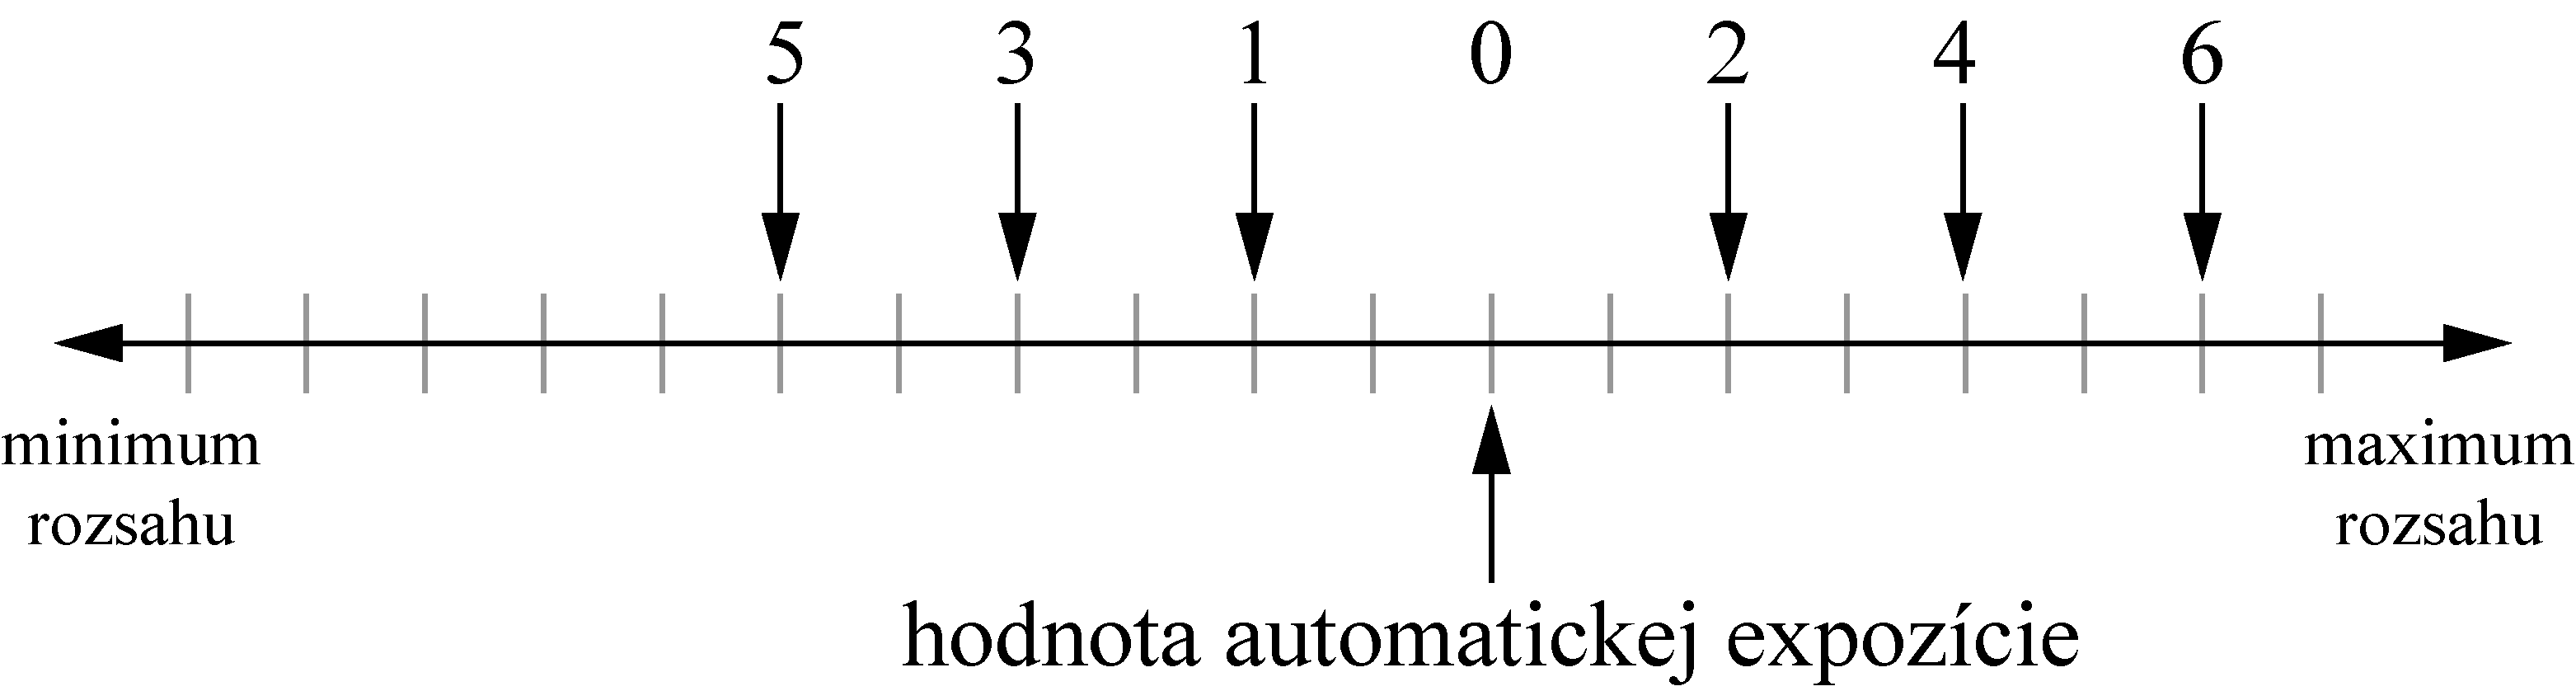
\includegraphics[width=0.7\textwidth]{figures/capturing/expoSelector0}
    \caption{Vyhľadávanie vhodných hodnôt časov expozície s krokom 2 (čísla zobrazujú poradie nájdených hodnôt)}
    \label{fig:expoSelector0}
\end{figure}

\begin{figure}[h!]
    \centering
    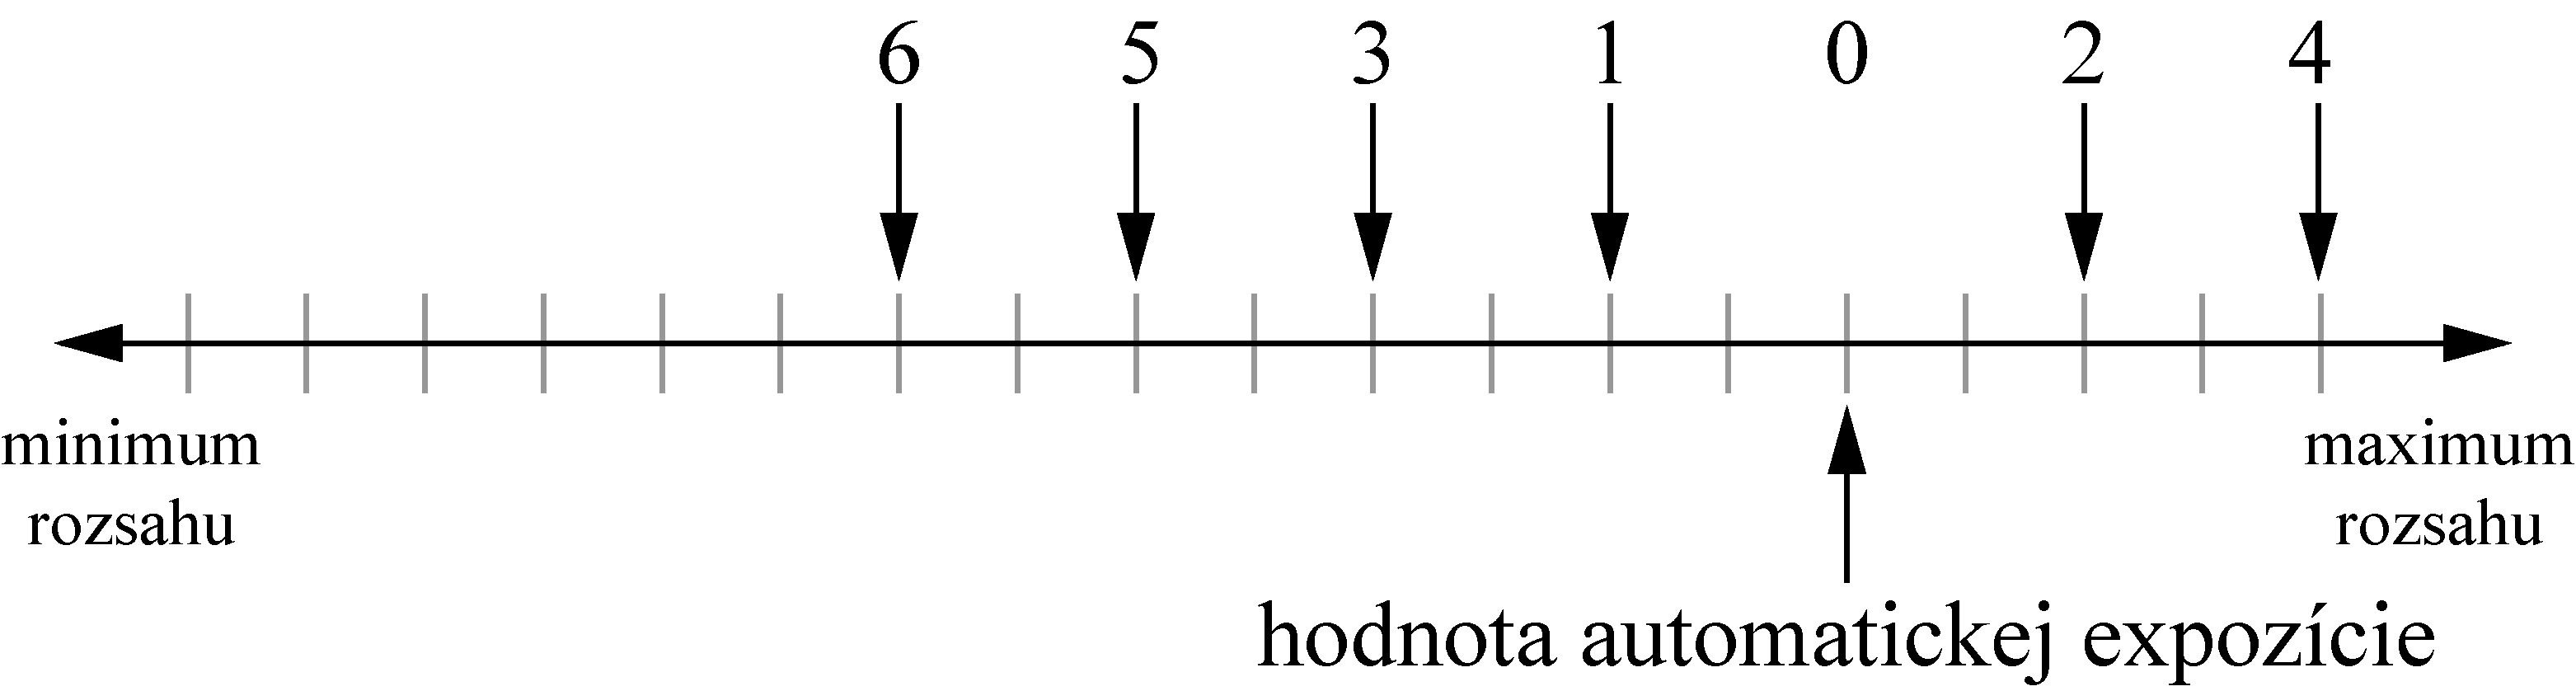
\includegraphics[width=0.7\textwidth]{figures/capturing/expoSelector1}
    \caption{Riešenie problému pri vysokej hodnote automatickej expozície}
    \label{fig:expoSelector1}
\end{figure}

\begin{algorithm}[]
    \SetAlgoLined
    \DontPrintSemicolon
    \caption{Výber expozičných časov}
    \label{algo_expositions}

    vstupy algoritmu:\;
    \texttt{  maxExpo} - maximálny počet expozícii\;
    \texttt{  krok} - krok pri výbere medzi expozičnými časmi v zozname \texttt{range}\;
    \texttt{  stredExpo} - hodnota automatickej expozície (najbližšia hodnota v tvare $2^{n}$)\;
    \;
    inicializácia premenných:\;
    \texttt{  stredIdx} = index hodnoty \texttt{stredExpo} v zozname \texttt{range}\;
    \texttt{  mensiIdx} = \texttt{stredIdx - krok}\;
    \texttt{  vacsiIdx} = \texttt{stredIdx + krok}\;
    \texttt{  pocet} - počet hodnôt v zozname \texttt{exposures}\;
    \texttt{  vacsiaHodnota} - booleanovská hodnota značiaca, či sa bude vyhľadávať menšia,
    alebo väčšia hodnota času expozície\;
    \texttt{  najdene} - booleanovská hodnota značiaca či sa v predchadzajúcom cykle našla vhodná hodnota\;
    \;
    vlož \texttt{stredExpo} do zoznamu \texttt{expozicie};\;
    \;
    \While{pocet < maxExpo}{
        \eIf{vacsiaHodnota}{
            \eIf{vacsiIdx <= najväčší index zoznamu range}{
                vlož hodnotu na indexe \texttt{vacsiIdx} zo zoznamu \texttt{range} do zoznamu \texttt{expozicie};\;
                \texttt{najdene} nastav na true;\;
                \texttt{vacsiIdx} inkrementuj o \texttt{krok};\;
                inkrementuj \texttt{pocet};\;
            }{
                ak sa v predchádzajúcom cykle nenašla vhodná hodnota - ukonči algoritmus;\;
                \texttt{najdene} nastav na false;\;
            }
            \texttt{vacsiaHodnota} nastav na false;\;
        }{
            \eIf{mensiIdx >= 0}{
                vlož hodnotu na indexe \texttt{mensiIdx} zo zoznamu \texttt{range} do zoznamu \texttt{expozicie};\;
                \texttt{najdene} nastav na true;\;
                \texttt{vacsiIdx} dekrementuj o \texttt{krok};\;
                inkrementuj \texttt{pocet};\;
            }{
                ak sa v predchádzajúcom cykle nenašla vhodná hodnota - ukonči algoritmus;\;
                \texttt{najdene} nastav na false;\;
            }
            \texttt{vacsiaHodnota} nastav na true;\;
        }
    }
\end{algorithm}

\subsection{Zarovnanie}
\label{sec:Practice-Alignment}

Jedným z predpokladov vytvárania HDR obsahu je statickosť zariadenia medzi fotografovaním jednotlivých expozícií.
Profesionálny fotograf si za normálnych okolností pri vytváraní HDR fotografie nasadí fotoaparát na statív.
Fotografovia používajú taktiež funkciu zvanú predsklopenie zrkadla (MLU\footnote{Mirror lock-up}) pre zníženie 
ďalších vibrácií. Problémy so zarovnaním sú oveľa horšie, ak sú zábery fotografované fotoaparátom vo voľnej ruke, 
alebo ako v našom prípade - fotografovaním pomocou smartfónu či tabletu.

Nezarovnanie snímok použitých pri vytváraní HDR obrazu môže mať za následok vážne artefakty. Na obrázku
\ref{fig:unaligned} môžeme vidieť artefakty nazývané ghosting (duchovia), ktoré majú vplyv na výsledný
obrázok. Ghosting nastáva aj v prípade, že sa na statickej scéne nachádza objekt, ktorý je voči scéne v pohybe.

\begin{figure}[h!]
    \centering
    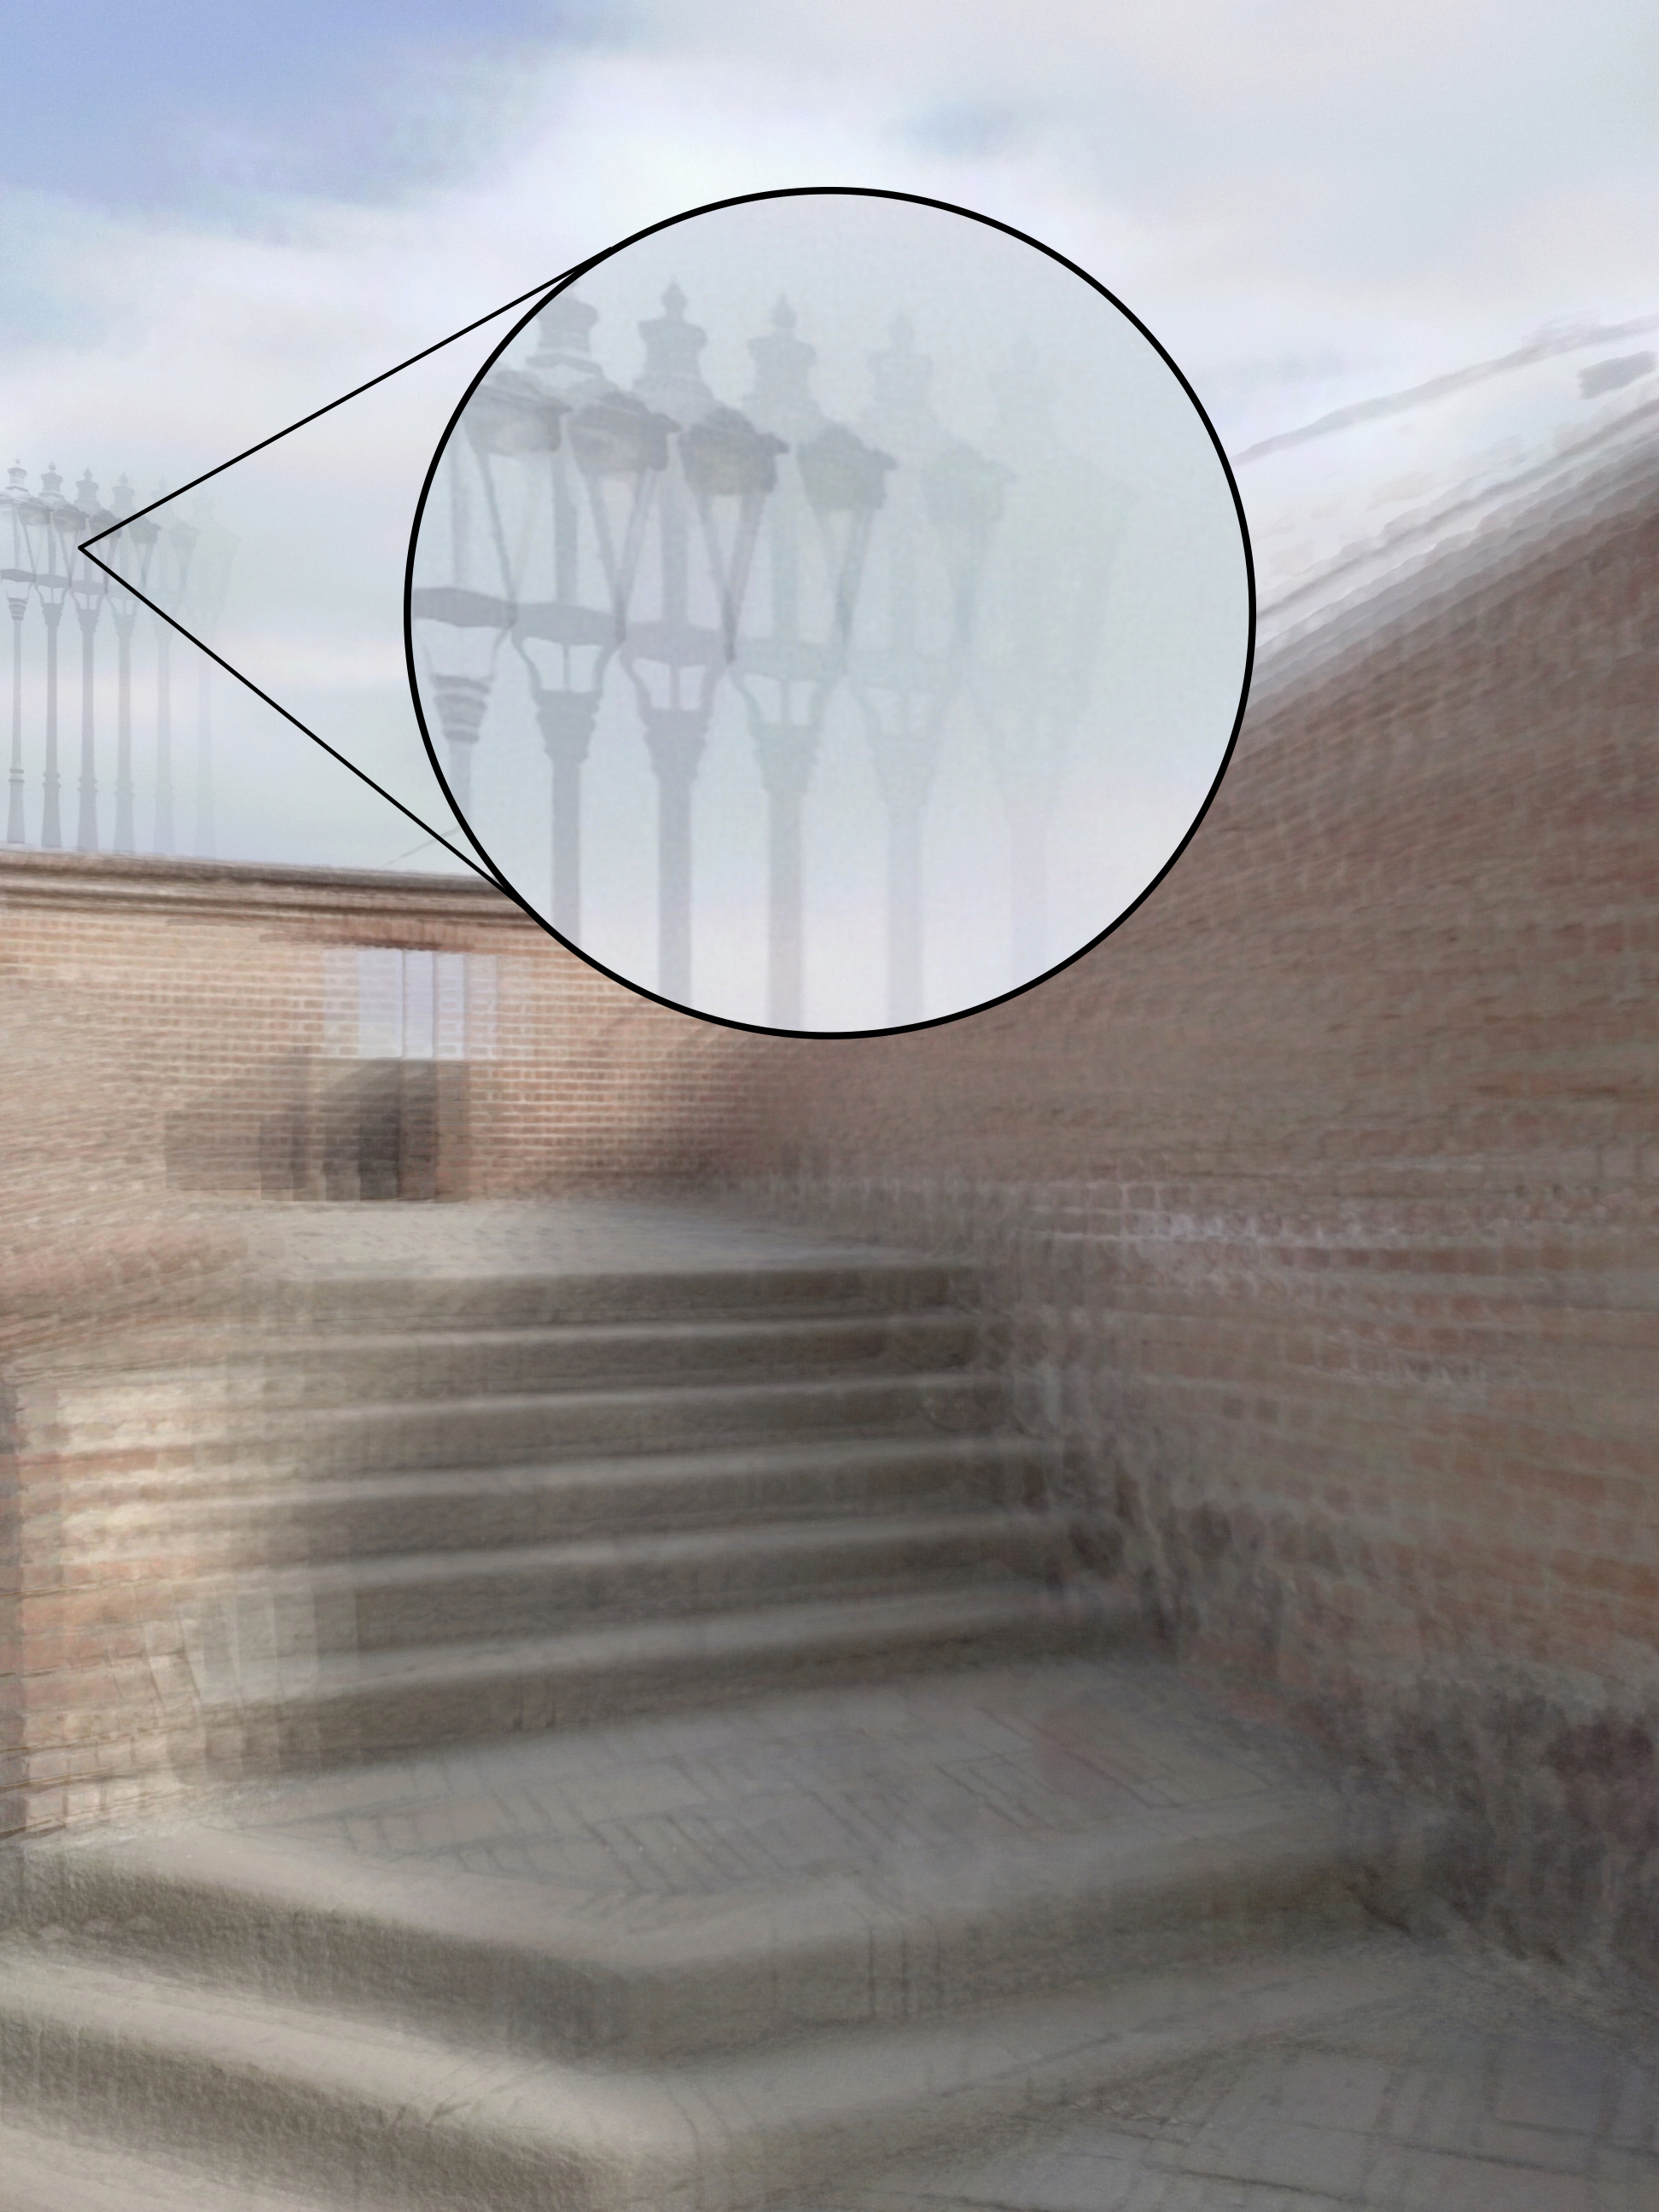
\includegraphics[width=0.3\textwidth]{figures/capturing/align/unaligned}
    \caption{Problémy vznikajúce pri nezarovnaní snímok}
    \label{fig:unaligned}
\end{figure}

\subsection*{Median threshold bitmap}

Pre zarovnanie vytvorených snímok je použitá metóda Grega Warda (2003), implementovaná v triede
\texttt{AlignMTB} knižnice OpenCV.

Vstupom metódy je zoznam vytvorených snímok, ktoré sú váženým priemerom prevedené na obrázky v stupňoch šedej.
Podľa histogramu jasu obrázkov sa určí 8-bitová hodnota mediánu a vytvoria sa MTB obrazy, kde každý pixel, ktorý 
je jasnejší než medián, má hodnotu 1 a v opačnom prípade hodnotu 0 \cite{Align}.

Metóda nepracuje s expozíciou snímok. Na obrázku \ref{fig:mtb} môžeme vidieť, že MTB obrazy sú pre rôzne expozície
skoro identické. Obrázky naľavo predstavujú vybrané snímky zo série expozicií scény a napravo sú ich príslušné
MTB obrazy.

\begin{figure}[t]
    \centering
    \begin{subfigure}{0.3\textwidth}
        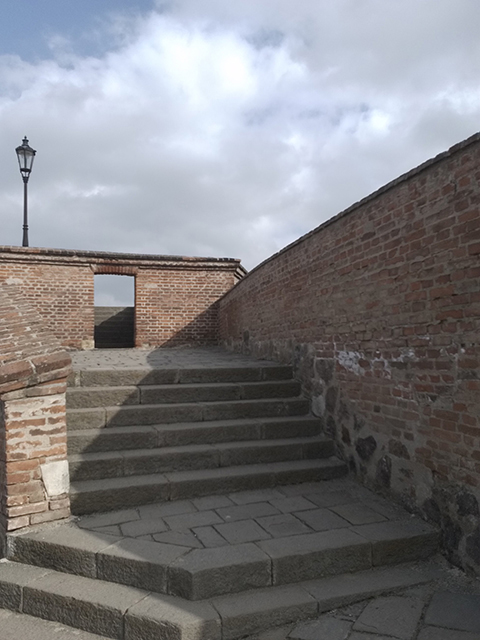
\includegraphics[width=\textwidth]{figures/capturing/align/image1}
    \end{subfigure}
    ~
    \begin{subfigure}{0.3\textwidth}
        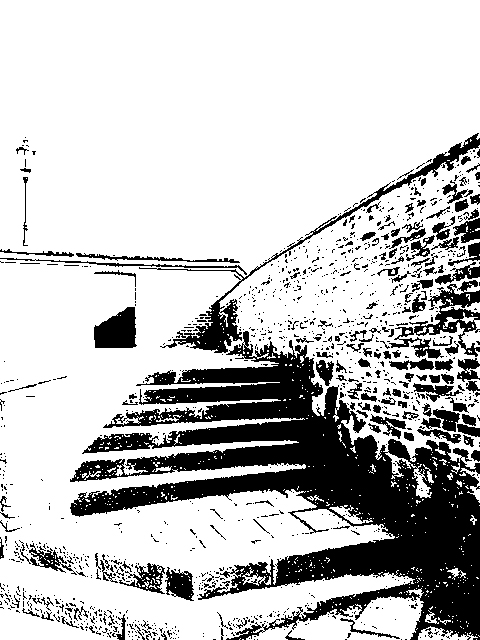
\includegraphics[width=\textwidth]{figures/capturing/align/image1tb}
    \end{subfigure}

    \begin{subfigure}{0.3\textwidth}
        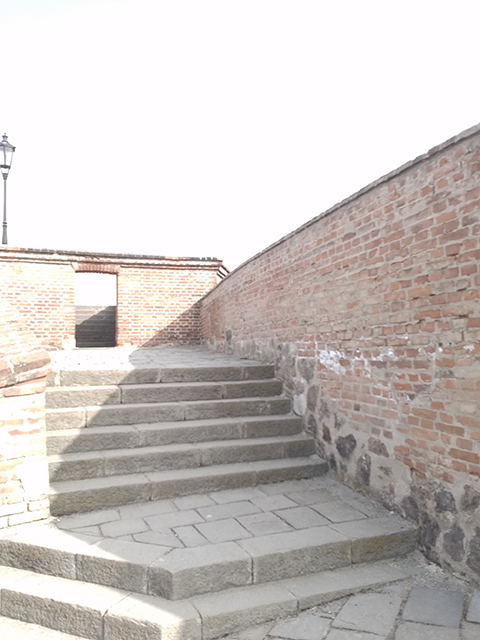
\includegraphics[width=\textwidth]{figures/capturing/align/image2}
    \end{subfigure}
    ~
    \begin{subfigure}{0.3\textwidth}
        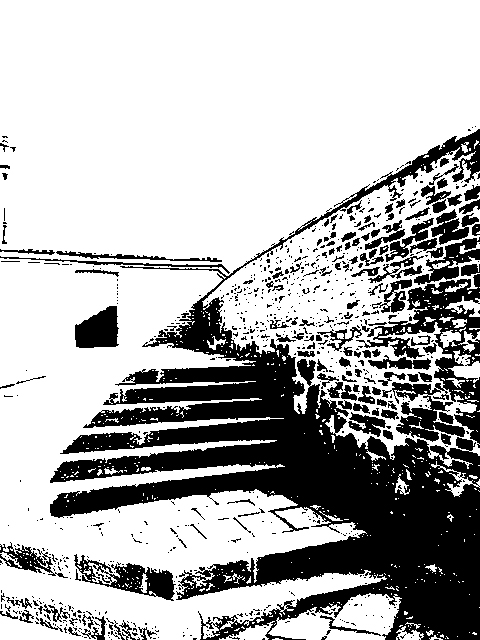
\includegraphics[width=\textwidth]{figures/capturing/align/image2tb}
    \end{subfigure}
    \caption{MTB obrazy vytvorené zo snímok z rozličným expozičným časom}
    \label{fig:mtb}
  \end{figure}

Jeden zo zoznamu obrázkov je zvolený za referenčný obrázok, podľa ktorého sa určujú číselné offsety zvyšných obrázkov.
Použitím XOR operátora môžeme na matici pixelov páru obrázkov jasne určiť offset nezarovnanosti na osiach $x$ a $y$.
Rýchlosť tejto metódy spočíva vo využívaní bitových operácií nad obrázkami, ktoré sú usporiadané v obrazovej pyramíde.
Offset sa začína určovať na páre obrázkov s najnižším rozlíšením. Postupne sa prechádza k~obrázkom s vyšším rozlíšením
a počíta sa odchýlka predchádzajúceho offsetu vynásobeného dvomi, čo zodpovedá zmene rozlíšenia.
Novovzniknuté oblasti obrazu sú vyplnené nulovými hodnotami.

\section{Generovanie HDR obsahu}

Potom, ako je fotoaparátom zariadenia zachytená séria snímok s rôzným expozičným časom, je potrebné tieto
obrázky zlúčiť do jedného HDR obsahu. Celý algoritmus spájania série snímok je obsiahnutý v triede
\texttt{HDRController}, ktorý dekomponuje problém do troch tried spomenutých v tejto kapitole. Pri zápise rovníc
a v zdrojovom kóde aplikácie sa nachádzajú premenné, ktorých význam je stručne popísaný v kapitole
\ref{sec:Theory-Generating}.

\subsection{Výber vzorky pixelov pre získanie krivky odozvy}

Pred generovaním samotného HDR obsahu si musíme vyjadriť krivku odozvy fotoaparátu a to riešením kvadratickej
objektívnej funkcie \ref{eq:objFunction}. Teoreticky by sa na riešene tejto rovnice mohol vziať každý pixel, 
každej expozície, ale to by bolo na výpočet veľmi časovo a priestorovo náročné. My však nepotrebujeme všetky
dostupné pixely. Ak máme $P$ fotografií po $N$ pixelov, výsledná intenzita žiarenia $E_{i}$ bude mať $N$ hodnôt
a krivka odozvy $g$ $(Z_{max} - Z_{min})$ hodnôt. Na úspešné vyriešenie rovnice nám stačí
$N(P - 1) > (Z_{max} - Z_{min})$\cite{Debevec} hodnôt. Tieto hodnoty však musíme vhodne vybrať zo sekvencie
expozícii.

Medzi dostupné metódy výberu pixelov pre získanie krivky odozvy môžeme zaradiť:
\begin{description}
  \item [Vyhľadávanie vhodných oblastí] je metóda spomenutá v knihe od E. Reinharda \cite{HDRI}. Metóda vyberá
  vhodné oblasti pomocou vylučovania vzoriek - vhodná oblasť je jasnejšia ako akákoľvek oblasť z predchádzajúcich
  expozícií, neprekrýva žiadnu inú oblasť a~má malú odchýlku v jase vlastných pixelov. Takto sa vyberá dostatočný
  počet oblastí od najjasnejšej po najtmavšiu expozíciu. V prípade, že tmavšie expozície nevyužívajú celý rozsah
  jasu je ťažké nájsť oblasti, ktoré sú jasnejšie ako na predchádzajúcej expozícii. To nejako významne neovplyvní
  výsledok, ale je dôležité stanoviť limit pri vylučovaní oblastí na jednej expozícii, aby sa algoritmus nedostal
  do nekonečného cyklu.

  \item [Výber pixelov pomocou histogramu] spočíva vo vytvorení histogramu hodnôt a počtu pixelov s týmito
  hodnotami pre jednotlivé expozície. Z každého histogramu boli nás-ledne vybrané hodnoty, ktoré pixely najčastejšie
  nadobúdali. Problémom metódy však je, že pri najtmavších expozíciách sú vybrané samé čierne pixely a pri svetlých
  expozíciách je to naopak. Kód zobrazuje tvorbu histogramu vytvoreného z jasovej zložky obrazu.
\begin{lstlisting}[]
histogram = new int[256];

for (int i = 0; i < jasovaZlozka.length; i++) {
  histogram[jasovaZlozka[i]] += 1;
}
\end{lstlisting}
  
  \item [Pravidelne usporiadané pixely] získame vybraním každého $n$-tého pixelu v určitom smere. Vyberať je možné
  prechádzaním riadkov, stĺpcov alebo diagonál. Metóda je veľmi efektívna najmä pri vhodne zvolenom kroku
  
  \item [Náhodný výber pixelov] je najjednoduchšou a často aj dostatočne efektívnou metódou. Táto metóda je
  implementovaná v triede \texttt{SamplesSelector}, ktorá pri inicializovaní vyjadrí potrebný počet hodnôt pixelov
  potrebných pre vyriešenie kvadratickej objektívnej rovnice.
\begin{lstlisting}[]
List<Integer> vybraneIndexy = new ArrayList<>();
int i = 0;

while (vybraneIndexy.size() < velkostVzorky) {
  // nahodny index pixelu
  int index = (int) Math.floor(Math.random() * pocetPixelov);

  if (!vybraneIndexy.contains(index)) {
    // nahodne vybrany index nemame vo vybranych
    for (int j = 0; j < pocetFotografii; j++) {
      // ulozit pixel na vybranom indexe
      vzorkaPixelov[i][j] = images.get(j).getPixel(index);
    }
    vybraneIndexy.add(idx);
    i++;
  }
}
\end{lstlisting}
  Z dôvodu zamedzenia nežiadúcemu stavu, že bude
  viackrát náhodne vybraný práve jeden pixel (čo je pri počte pixelov na fotografii málo pravdepodobné),
  je definované pole vybraných indexov. Vhodný index je taký, ktorý sa nenachádza v poli už vybraných indexov.
\end{description}

\begin{figure}[t]
  \centering
  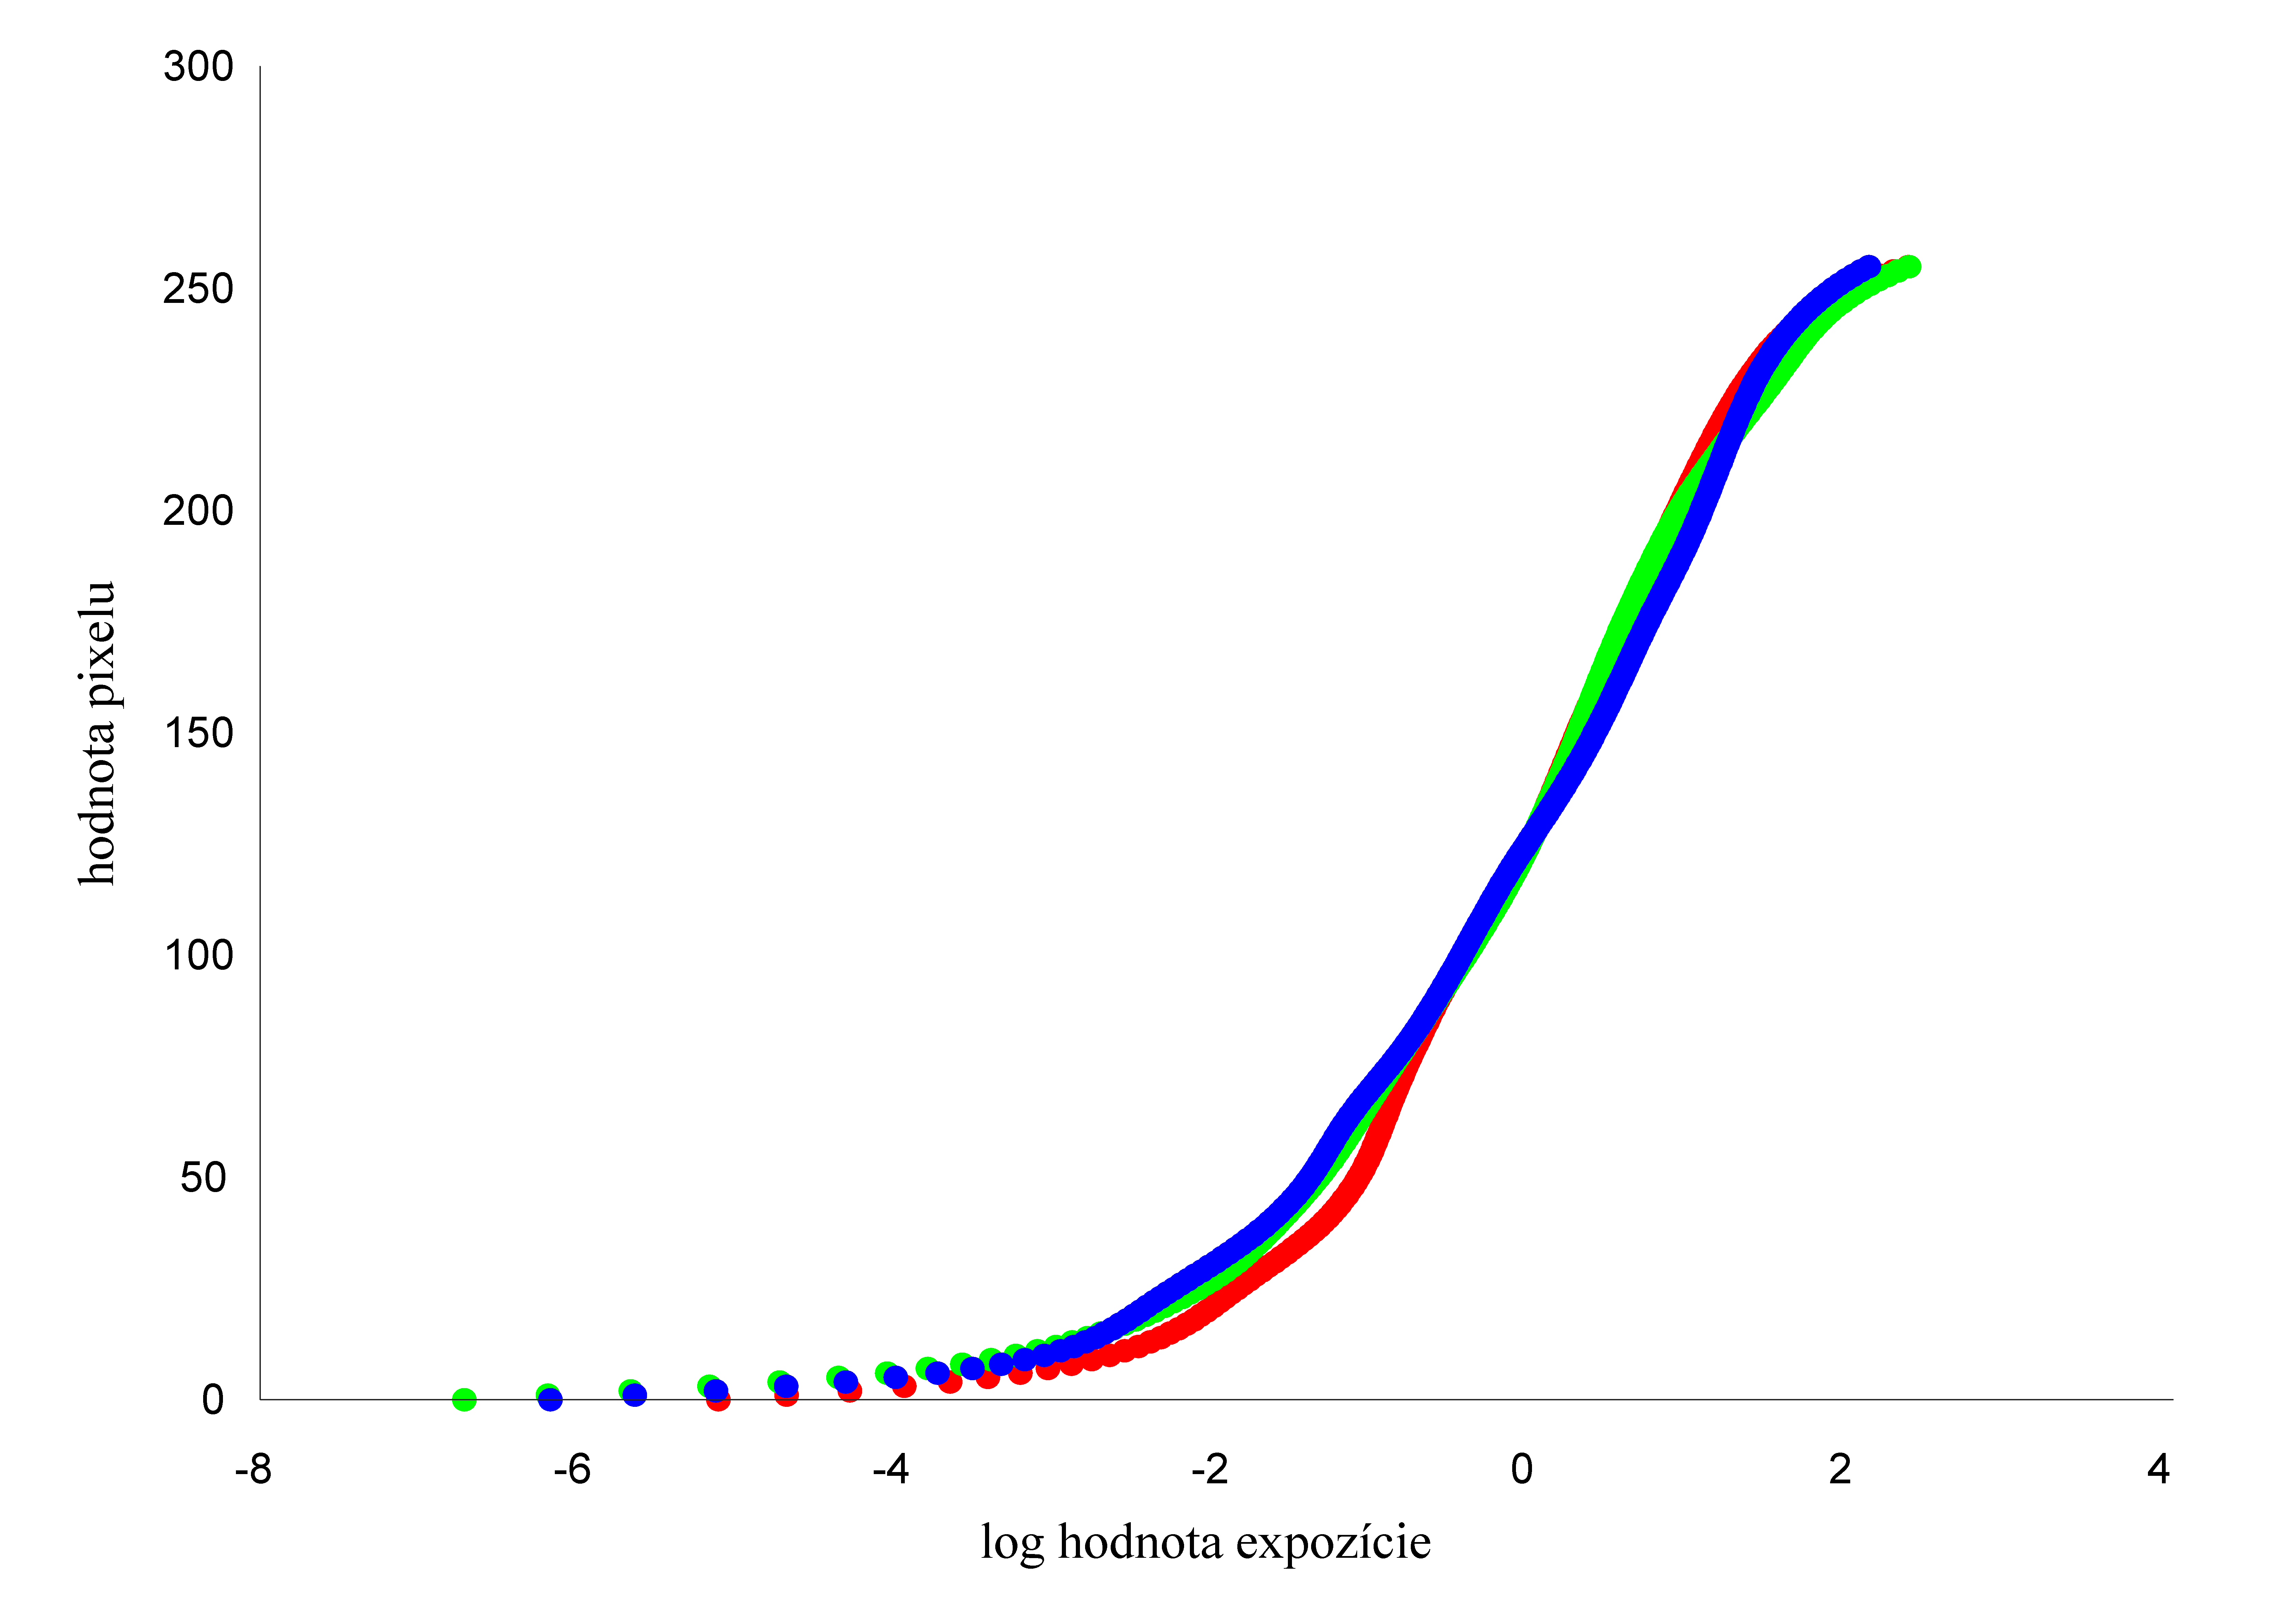
\includegraphics[width=0.9\textwidth]{figures/generating/octave-crf}
  \caption{Graf CRF kriviek jednotlivých farebných kanálov}
  \label{fig:octave_crf}
\end{figure}

\subsection{Získanie krivky odozvy fotoaparátu}

Ak máme vybrané dostatočné množstvo hodnôt, môžeme riešiť objektívnu kvadratickú rovnicu \ref{eq:objFunction}.
Rovnica je doplnená o váhovú funkciu \ref{eq:weightFunction}, pomocou ktorej dosiahneme, že hodnoty v okolí
$Z_{mid}$ budú mať väčšiu váhu ako hodnoty v okolí $Z_{min}$ a $Z_{max}$. $Z_{mid}$ je prostredná hodnota rozsahu
hodnôt pixelu, vyjadrená ako $Z_{mid} = \frac{1}{2}(Z_{min} + Z_{max})$. Túto hodnotu je potrebné nastaviť na 0.

\begin{equation} \label{eq:weightFunction}
  w(z)=
  \begin{cases}
    z - Z_{min}, & \text{pre}\ z \leq \frac{1}{2}(Z_{min} + Z_{max}) \\
    Z_{max} - z, & \text{pre}\ z > \frac{1}{2}(Z_{min} + Z_{max})
  \end{cases}
  \cite{Debevec}
\end{equation}

Keďže aplikácia pracuje s farebnými obrázkami, musíme vyjadriť krivku odozvy $g$ pre každý farebný kanál (obr. \ref{fig:octave_crf}).
Pridaním váhovej funkcie sa rovnica \ref{eq:objFunction} z podkapitoly \ref{sec:Theory-Generating} upraví na~tvar:
\begin{equation} \label{eq:rrFunction}
        \mathcal{O} = 
        \sum_{i=1}^{N}
        \sum_{j=1}^{P}
        \big (w(Z_{ij})[g(Z_{ij}) - \ln E_{i} - \ln \Delta t_{j}] \big )^{2}
        + \lambda
        \sum_{z=Z_{min} + 1}^{Z_{max} - 1}
        [w(z) g''(z)]^{2}
        \cite{Debevec}
\end{equation} 

Trieda \texttt{CRFRecover} implementuje riešenie tejto rovnice na základe ukážky \texttt{MATLAB} kódu od Paula
E. Debeveca a J. Malika\cite{Debevec}. Kód bol
debugovaný pomocou voľne šíriteľného softvéru GNU Octave\footnote{\url{www.gnu.org/software/octave/}}
a následne implementovaný v Jave. Na záver je potrebné vykonať dekompozíciu vytvorených matíc. Dekompozícia
je realizovaná pomocou metódy SVD\footnote{Singular-value decomposition},
z knižnice OpenCV.

\subsection{Vytvorenie funkcie žiarenia}

Ak už máme vyjadrenú krivku odozvy $g$, vieme ju použiť na prepočet hodnoty pixelu na~relatívnu hodnotu žiarenia.
Riešením rovnice \ref{eq:gFunction} a pridaním váhovej funkcie \ref{eq:weightFunction} získame rovnicu:
\begin{equation}
    \ln E_{i} = 
    \frac{
        \sum_{j=1}^{P}
        w(Z_{ij})(g(Z_{ij}) - \ln \Delta t_{j})
    }{
        \sum_{j=1}^{P}
        w(Z_{ij})
    }
    \cite{Debevec}
\end{equation}
Na generovanie HDR obsahu potrebujeme vyjadriť $\ln E_{i}$ pre každý pixel a každý farebný kanál. Vyjadrená
hodnota pixelu v logaritmickom tvare sa musí upraviť na základný tvar $E_{i}$ pomocou inverznej funkcie
$e^{x}$. Na záver sú tieho hodnoty funkcie žiarenia zlúčené do matice \texttt{org.opencv.core.Mat} typu
\texttt{CvType.CV\_32FC3}, čo značí maticu 32-bitových hodnôt s pohyblivou rádovou čiarkou pre 3 farebné kanály.
Tento algoritmus je implementovaný v~triede \texttt{HDRMerge}.

\section{Prevod HDR obsahu na LDR}

Dostali sme sa do stavu, kedy máme vytvorený HDR obsah z $n$ nasnímaných fotografií. Tento obsah je nutné vhodne užívateľovi prezentovať.
Po vytvorení HDR obsahu sa preto zobrazí obrazovka, na ktorej je zoznam implementovaných operátorov mapovania tónov s~ich náhľadom.
Jednotlivé operátory mapovania tónov sú implementované pomocou knižnice OpenCV, ktorá poskytuje globálne operátory \texttt{Reinhard},
\texttt{Drago} a lokálne operátory \texttt{Durand} a \texttt{Mantiuk}.

\subsection{Operátory mapovania tónov}

Ak si užívateľ vyberie jeden zo zoznamu ponúkaných operátorov mapovania tónov, zob-razí sa obrazovka pre editovanie parametrov operátora.
Obrazovka obsahuje posuvníky (\texttt{SeekBar}) parametrov, ktoré operátor umožňuje nastavovať na vstupe. Parametre majú definovaný svoj
platný rozsah a východzie hodnoty pre optimálny výsledok, ktoré sú vymenované v enume \texttt{TmoParams}. Keďže parametre na vstupe metódy
môžu mať rozličný rozsah v obore reálnych čísel, ale posuvník môže nadobudnúť iba hodnoty v rozsahu 0 - 100, musia sa tieto absolútne hodnoty
prevádzať na relatívne hodnoty v rozsahu posuvníka. Enum \texttt{TmoParams} obsahuje východzie hodnoty parametrov operátorov v absolútnom
a relatívnom tvare a metódu na prevod relatívnej hodnoty zadanej užívateľom na posuvníku na absolútnu hodnotu pre vstup metódy. Viac o týchto
parametroch je popísané v tabuľke \ref{table:tmoParams}.

Každý posuvník na obrazovke má vlastný callback \texttt{OnSeekBarChangeListener}, ktorý pri manipulovaní s posuvníkom vracia v metóde
\texttt{onProgressChanged} objekt \texttt{SeekBar} s~aktuálnymi nastaveniami posuvníka. Z tohoto objektu sme schopní vybrať hodnotu posuvníka
v rozsahu 0 - 100, túto hodnotu previesť na absolútnu hodnotu pre metódu operátora mapovania tónov a nakoniec zobraziť výsledný obrázok.

Okrem posuvníkov obsahuje obrazovka náhľadový obrázok a tlačidlá pre uloženie HDR obsahu a výslednej LDR fotografie, tlačidlo pre resetovanie
nastavení posuvníkov na východzie hodnoty a tlačidlo pre otočenie náhľadového obrázku.

\begin{table}[t]
  \centering
  \begin{tabular}{||c|m{14em}|m{6em}|c|m{4.2em}||} 
    \hline
    Parameter 
    & \makecell{Popis}
    & \makecell{Operátor}
    & \makecell{Rozsah}
    & \makecell{Východzia\\hodnota} \\
    \hline\hline
    gamma
    & \makecell{hodnota gama korekcie}
    & \makecell{všetky\\operátory}
    & \makecell{1.0 - 3.0}
    & \makecell{2.2} \\
    \hline
    saturation
    & \makecell{hodnota sýtosti farieb }
    & \makecell{Drago,\\Durand,\\Mantiuk}
    & \makecell{0.0 - 4.0}
    & \makecell{1.0} \\
    \hline
    scale
    & \makecell{faktor kontrastu, ktorým sa\\násobí hodnota vizuálnej\\odozvy, čím sa komprimuje\\dynamický rozsah}
    & \makecell{Mantiuk}
    & \makecell{0.6 - 0.9}
    & \makecell{0.7} \\
    \hline
    intensity
    & \makecell{intenzita svetla\\vo výslednom obraze}
    & \makecell{Reinhard}
    & \makecell{-8.0 - 8.0}
    & \makecell{0.0} \\
    \hline
    light adapt
    & \makecell{prispôsobenie svetla\\(1 = adaptácia je počítaná iba\\z hodnoty pixelu)}
    & \makecell{Reinhard}
    & \makecell{0.0 - 1.0}
    & \makecell{0.0} \\
    \hline
    color adapt
    & \makecell{prispôsobenie farieb\\(1 = farebné kanály\\sú spracované nezávisle)}
    & \makecell{Reinhard}
    & \makecell{0.0 - 1.0}
    & \makecell{0.0} \\
    \hline
    contrast
    & \makecell{výsledný kontrast\\v logaritmickej mierke\\($\ln{\frac{max}{min}}$ hodnoty\\jasu výsledného obrazu)}
    & \makecell{Durand}
    & \makecell{0.0 - 8.0}
    & \makecell{4.0} \\
    \hline
    sigma space
    & \makecell{hodnota bilaterálneho filtra\\v súradnicovom priestore}
    & \makecell{Durand}
    & \makecell{0.0 - 4.0}
    & \makecell{2.0} \\
    \hline
    sigma color
    & \makecell{hodnota bilaterálneho filtra\\vo farebnom priestore}
    & \makecell{Durand}
    & \makecell{0.0 - 4.0}
    & \makecell{2.0} \\
    \hline
    bias
    & \makecell{hodnota pre funkciu bias}
    & \makecell{Drago}
    & \makecell{0.0 - 1.0}
    & \makecell{0.85} \\
    \hline
  \end{tabular}
  \caption{Hodnoty a rozsahy parametrov operátorov mapovania tónov \cite{OpenCV}}
  \label{table:tmoParams}
\end{table}

\subsection{Zmenšenie náhľadového obrázku}

Operátory mapovania tónov sa pre náhľadové obrázky aplikujú na zmenšený HDR obsah. To zaručí menšiu časovú náročnosť zobrazenia
obrazovky s operátormi mapovania tónov. Zmenšenie náhľadového obrázku je implementovaná pomocou metódy \texttt{resize} triedy \texttt{Imgproc}
knižnice OpenCV, využitím bilineárnej interpolácie. Na obrazovke vybraného operátora mapovania tónov, kde je možné modifikovať
vstupné parametre algoritmu, môže byť vďaka zmenšeniu zobrazovaný náhľad v reálnom čase bez väčších oneskorení.

\section{Ukladanie}

V závere celého procesu vytvárania HDR fotografie musí byť užívateľ schopný uložiť si výsledok. Aplikácia ponúka
uloženie nielen výslednej fotografie v štandardnom obrazovom formáte \texttt{JPEG}, ale aj uloženie HDR obsahu 
pre neskoršiu editáciu. V tomto prípade je HDR obsah komprimovaný kódovaním RGBE, ktorý je popísaný v podkapitole
\ref{section-formats} Formáty HDR obsahu. Uloženie HDR formátu je veľkou výhodou, ktorú neponúka žiadna z aplikácií
prieskumu. Užívateľ sa totiž nemusí práve nachádzať v situácii, kedy si nájde čas na vhodné prispôsobenie výsledných
parametrov LDR obrazu.

Kódovanie HDR obsahu je implementované prostredníctvom modulu \texttt{imgcodecs} knižnice OpenCV, konkrétne funkciou
\texttt{imwrite}. Následné načítanie \texttt{.hdr} súboru sa vykonáva pomocou funkcie \texttt{imread}.
Užívateľ môže k uloženým HDR súborom pristupovať kedykoľvek z domovskej obrazovky aplikácie kliknutím na tlačidlo
"Load". Po zvolení tejto možnosti sa zobrazí obrazovka, ktorá obsahuje výpis (\texttt{ListView}) uložených
\texttt{.hdr} súborov v zariadení užívateľa. Výberom jedného z ponúkaných súborov sa súbor načíta a zobrazí 
sa obrazovka pre editáciu HDR obsahu.

Pri vstupno-výstupných operáciách nad úložiskom zariadenia je potrebné získať cestu typu \texttt{java.io.File}.
Na to slúži trieda \texttt{Storages}, ktorá obsahuje statické metódy pre získanie cesty, vrátane vytvorenia
potrebných priečinkov a kontroly, či daná operácia neprepíše existujúci súbor.

Pri ukladaní HDR obsahu alebo LDR výslednej fotografie je užívateľ pomocou dialógového okna vyzvaný, aby do textového
poľa vložil názov svojho nového súboru (obr. \ref{fig:saveDialog}). Z hľadiska funkcionality, sa vytvorí nová inštancia
triedy \texttt{SaveDialog}, ktorá je rozšírená o funkcionalitu triedy \texttt{DialogFragment}. V metóde \texttt{onCreateDialog}
sa pomocou \texttt{AlertDialog.Builder} vytvoria komponenty rozhrania dialógového okna. Príponu ukladaného súboru nevolí
užívateľ, ale je zvolená aplikáciou podľa formátu, v akom bude súbor uložený.

\begin{figure}[h!]
  \centering
  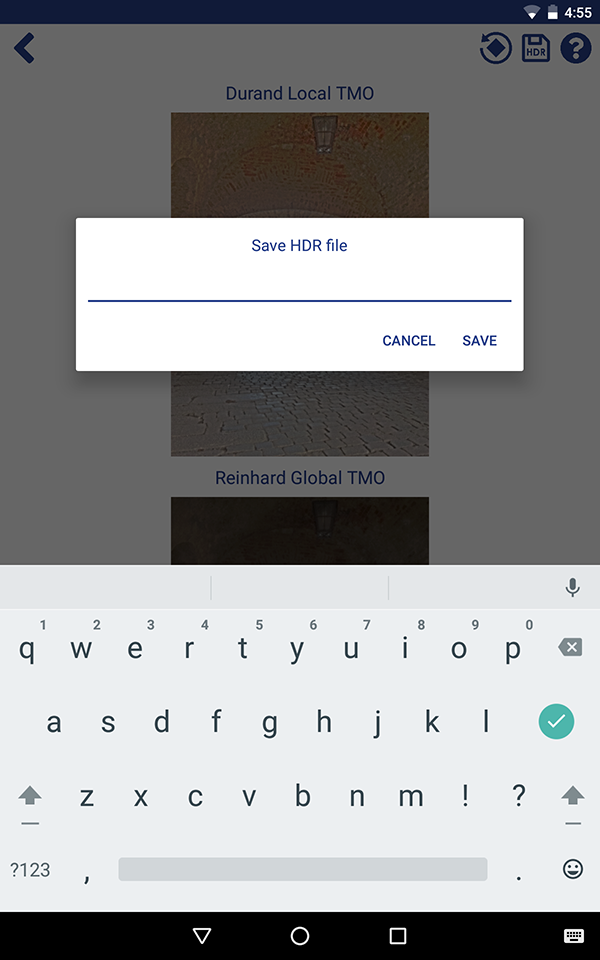
\includegraphics[width=0.35\textwidth]{figures/storage/dialogs/saveHdr}
  % 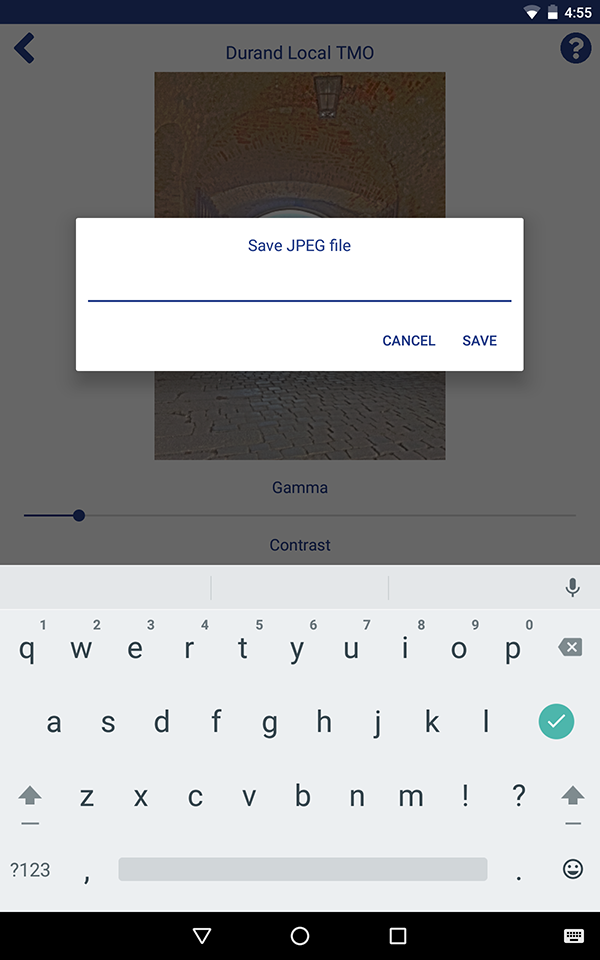
\includegraphics[width=0.3\textwidth]{figures/storage/dialogs/saveJpeg}
  \caption{Dialógové okno pre uloženie súboru vo formáte \texttt{.hdr}}
  \label{fig:saveDialog}
\end{figure}

\subsection*{Úložiská Android zariadenia}

Systém Android ponúka niekoľko možností pre uloženie dát aplikácie. Výber závisí od pot-rieb aplikácie, napríklad
od objemu dát alebo od prístupnosti dát iným aplikáciám. Dos-tupné možnosti uloženia dát v zariadení sú \cite{Android}:
\begin{itemize}
  \item Interné úložisko zariadenia - privátne súbory aplikácie v zariadení.
  \item Externé úložisko zariadenia - zdieľaný súborový systém zariadenia.
  \item Lokálne úložisko - ukladanie neobjemných dát typu kľúč, hodnota.
  \item Databázy - uloženie štruktúrovaných údajov do súkromnej SQLite databázy.
\end{itemize}

Pre ukladanie dát aplikácie je využité externé úložisko. Toto úložisko je vhodným miestom pre súbory, ktoré
nevyžadujú ombedzenia prístupu a pre súbory, ktoré majú byť zdieľané s inými aplikáciami alebo viditeľné pri
prenose súborov do počítača. Výsledné HDR fotografie by mali byť prístupné aj pre iné aplikácie v zariadení
a súbory formátu \texttt{.hdr} môžu vyžadovať viac pamäte, preto je ich vhodné ukladať do externého úložiska. 
Externé úložisko nemusí byť stále k~dispozícii, keďže môže byť obsiahnuté na úložnom médiu ako napríklad SD karte.
Aplikácii, pracujúcej s externým úložiskom, musia byť užívateľom udelené povolenia \texttt{WRITE\_EXTERNAL\_STORAGE} 
a \texttt{READ\_EXTERNAL\_STORAGE}.

V prípade, ak by aplikácia ukladala krivku odozvy fotoaparátu, ktorá je špecifická pre snímač zariadenia, dáta
by sa uložili na interné úložisko. Interné úložisko zariadenia je k~dispozícii nepretržite. Súbor je prístupný
iba danej aplikácii a po odinštalovaní aplikácie systém odstráni všetky súbory aplikácie z interného úložiska.

\chapter{Merania a výsledky}
Na testovanie mobilnej aplikácie bolo zachytených 6 scén. Každú scénu tvorí 11 snímok od~najtmavšej po najsvetlejšiu
expozíciu. Scéna \textit{brana} (obr. \ref{fig:BranaSeries}) je najlepším reprezentantom scény s vysokým dynamickým
rozsahom a je použitá pri väčšine testovaní a porovnávaní. Scéna \textit{brana} a scény \textit{lavicka}, \textit{park},
\textit{petrov}, \textit{schody}, \textit{vyhliadka} sú vo formáte \texttt{.hdr} súčasťou odovzdávanej práce. Každá scéna
je význačná rôznymi, pre prácu prínosnými vlastnosťami.

\begin{figure}[t]
  \centering
  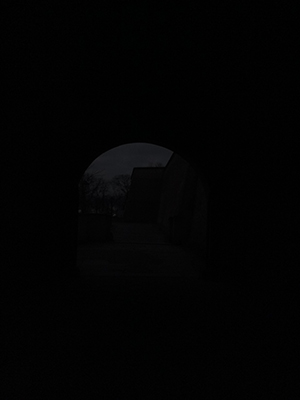
\includegraphics[width=0.08\textwidth]{figures/capturing/series/s0}
	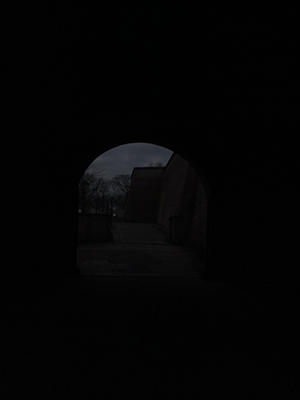
\includegraphics[width=0.08\textwidth]{figures/capturing/series/s1}
	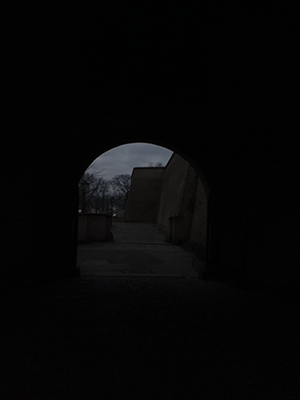
\includegraphics[width=0.08\textwidth]{figures/capturing/series/s2}
	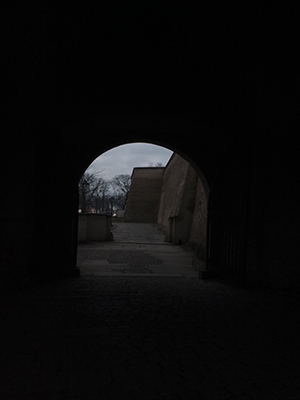
\includegraphics[width=0.08\textwidth]{figures/capturing/series/s3}
	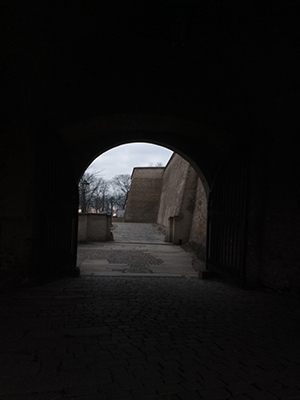
\includegraphics[width=0.08\textwidth]{figures/capturing/series/s4}
	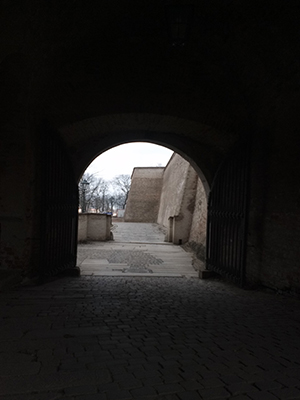
\includegraphics[width=0.08\textwidth]{figures/capturing/series/s5}
	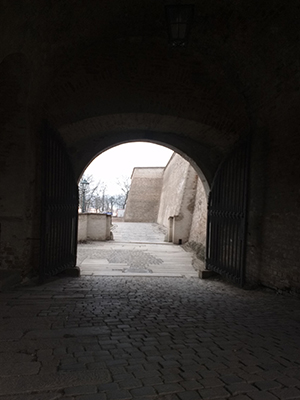
\includegraphics[width=0.08\textwidth]{figures/capturing/series/s6}
	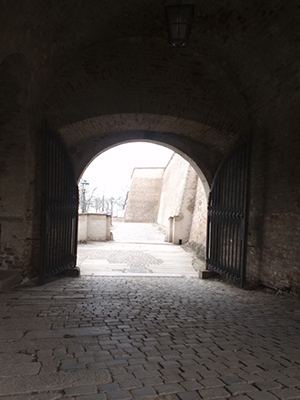
\includegraphics[width=0.08\textwidth]{figures/capturing/series/s7}
	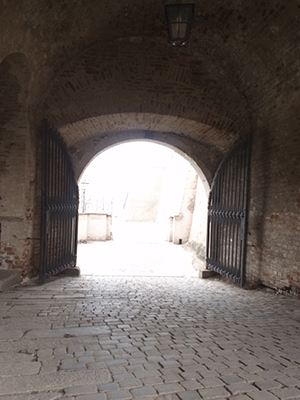
\includegraphics[width=0.08\textwidth]{figures/capturing/series/s8}
	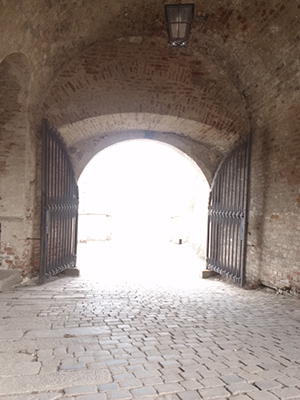
\includegraphics[width=0.08\textwidth]{figures/capturing/series/s9}
	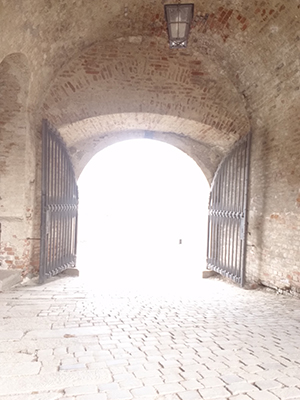
\includegraphics[width=0.08\textwidth]{figures/capturing/series/s10}
  \caption{Séria 11 snímok scény \textit{brana} zachytených s rôznym expozičným časom}
  \label{fig:BranaSeries}
\end{figure}

Pre vytváranie aplikácie, snímanie fotografií scén a záverečné testovanie je použitý tablet SHIELD NVIDIA s operačným
systémom Android 7.0 Nougat. Fotoaparát tabletu má rozlíšenie 5 Mpx a vytvorené snímky rozmer $1944\times2592$ px.
Z pohľadu užívateľa sú bežné fotografie vytvárané týmto zariadením uspokojivé, ale nie dokonalé. Digitálny snímač
nedokáže obsiahnúť taký rozsah farieb a jasu ako štandardný optický fotoaparát. Rozsah expozičného času snímača
tabletu je od 33 600 $ns$ do 356 732 928 $ns$.
\section{Výsledky operátorov mapovania tónov}

Testované scény boli hodnotené a porovnávané pri použití rôzných nastavení pre štyri operátory mapovania tónov.
Globálne operátory \texttt{Reinhard} a \texttt{Drago} neumožňujú na scéne s vysokým dynamickým rozsahom získať uspokojivý
výsledok, kde by boli jasne viditeľné zároveň tmavé a svetlé oblasti. Na prvých dvoch obrázkoch \ref{fig:reinhards}
máme dobre viditeľnú svetlú časť scény, no keď chceme pridať jas aj na tmavej časti, svetlá časť sa preexponuje
(tretí obrázok).

\begin{figure}[h!]
  \centering
  \begin{subfigure}{0.3\textwidth}
      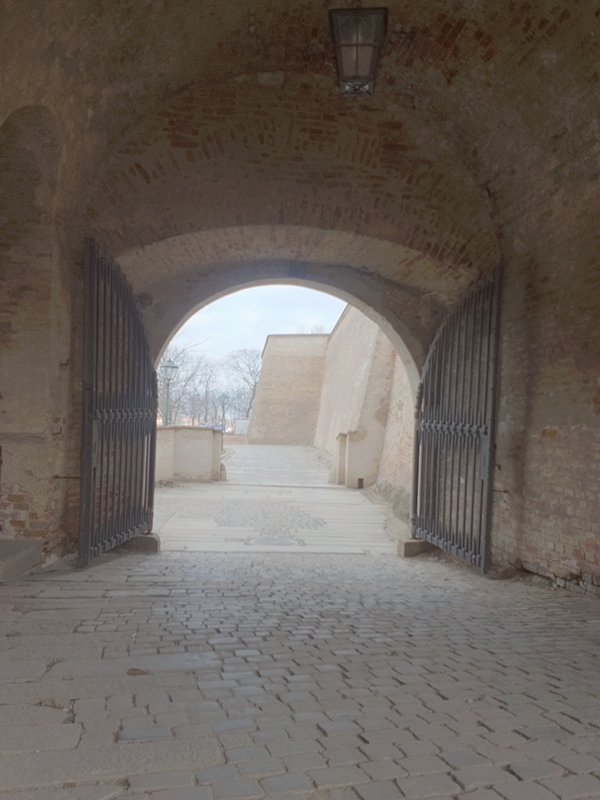
\includegraphics[width=\textwidth]{figures/tests/tmo/rein1}
  \end{subfigure}
  ~
  \begin{subfigure}{0.3\textwidth}
      \includegraphics[width=\textwidth]{figures/tests/tmo/rein2}
  \end{subfigure}
  ~
  \begin{subfigure}{0.3\textwidth}
    \includegraphics[width=\textwidth]{figures/tests/tmo/rein4}
  \end{subfigure}
  \caption{Výsledky mapovania tónov Reinhardovým operátorom}
  \label{fig:reinhards}
\end{figure}

Operátor \texttt{Drago} dokáže scénu s vysokým dynamickým rozsahom spracovať o niečo lepšie.
Jedinou užívateľom definovateľnou hodnotou je hodnota skreslenia (bias). Menšie hodnoty vytvárajú výrazne svetlejšie
snímky. Pri hodnotách, ktoré sa blížia minimu rozsahu nastáva na svetlých častiach nežiadúci stav - inverzia tónov,
zobrazená na treťom obrázku \ref{fig:dragos}.

\begin{figure}[h!]
  \centering
  \begin{subfigure}{0.3\textwidth}
      \includegraphics[width=\textwidth]{figures/tests/tmo/drag1}
  \end{subfigure}
  ~
  \begin{subfigure}{0.3\textwidth}
      \includegraphics[width=\textwidth]{figures/tests/tmo/drag3}
  \end{subfigure}
  ~
  \begin{subfigure}{0.3\textwidth}
      \includegraphics[width=\textwidth]{figures/tests/tmo/drag2}
  \end{subfigure}
  \caption{Výsledky mapovania tónov operátorom Drago}
  \label{fig:dragos}
\end{figure}

Lokálny operátor \texttt{Mantiuk} neponúka množstvo možností definovania vstupných parametrov. Aj preto možno užívateľ
nedokáže nájsť vhodné hodnoty nastavení, ktoré pre svoju scénu s vysokým dynamickým rozsahom potrebuje (obr.
\ref{fig:mantiuks}).

\begin{figure}[h!]
  \centering
  \begin{subfigure}{0.3\textwidth}
      \includegraphics[width=\textwidth]{figures/tests/tmo/man3}
  \end{subfigure}
  ~
  \begin{subfigure}{0.3\textwidth}
      \includegraphics[width=\textwidth]{figures/tests/tmo/man4}
  \end{subfigure}
  \caption{Výsledky mapovania tónov operátorom Mantiuk}
  \label{fig:mantiuks}
\end{figure}

Najlepšie výsledky ponúka užívateľovi lokálny operátor \texttt{Durand}. Zo všetkých operátorov ponúka užívateľovi
najviac možností editovania vstupných parametrov. Pomocou nastavenia kontrastu môže užívateľ dobre definovať pomer výsledných
hodnôt jasu a tak vytvárať obrazy verne zobrazujúce scénu alebo obrazy s umeleckým efektom (obr. \ref{fig:durandUsage}).
Nastavovaním hodnôt bilaterálneho filtra \texttt{sigma color} a \texttt{sigma space} užívateľ zdôrazňuje detaily scény.

\begin{figure}[h!]
  \centering
  \begin{subfigure}{0.3\textwidth}
      \includegraphics[width=\textwidth]{figures/tests/tmo/dur2}
  \end{subfigure}
  ~
  \begin{subfigure}{0.3\textwidth}
      \includegraphics[width=\textwidth]{figures/tests/tmo/dur3}
  \end{subfigure}
  ~
  \begin{subfigure}{0.3\textwidth}
      \includegraphics[width=\textwidth]{figures/tests/tmo/dur5}
  \end{subfigure}
  \caption{Výsledky mapovania tónov operátorom Durand}
  \label{fig:durands}
\end{figure}

\begin{figure}[h!]
  \centering
  \begin{subfigure}{0.3\textwidth}
      \includegraphics[width=\textwidth]{figures/tests/tmo/durSpace1}
      \caption{Vyhladenie}
  \end{subfigure}
  ~
  \begin{subfigure}{0.3\textwidth}
      \includegraphics[width=\textwidth]{figures/tests/tmo/durSpace2}
      \caption{Zvýraznenie detailov}
  \end{subfigure}
  ~
  \begin{subfigure}{0.3\textwidth}
      \includegraphics[width=\textwidth]{figures/tests/tmo/durVerna2}
      \caption{Verné zobrazenie scény}
  \end{subfigure}
  \caption{Obrazy verne zobrazujúce scénu ale aj umelecké efekty}
  \label{fig:durandUsage}
\end{figure}

Pri vysokých hodnotách \texttt{sigma color} a zároveň \texttt{sigma space} nastáva na hrane svetlej a tmavej oblasti halo efekt.
Operátor zahrnie pri výpočte blízko takejto hrany aj druhú stranu prechodu a zvýši kontrast naprieč hranou. Halo efekt je v
profesionálnej fotografii považovaný za chybu pri zobrazovaní reálnej scény. Veľa amatérskych fotografov však považuje toto
skreslenie ako súčasť umeleckého efektu fotografie.

\begin{figure}[h!]
  \centering
  \begin{subfigure}{0.3\textwidth}
      \includegraphics[width=\textwidth]{figures/tests/tmo/durHalo1}
  \end{subfigure}
  ~
  \begin{subfigure}{0.3\textwidth}
      \includegraphics[width=\textwidth]{figures/tests/tmo/durHalo2}
  \end{subfigure}
  \caption{Halo efekt spôsobený ostrým prechodom medzi zreteľne svetlou a tmavou oblasťou}
  \label{fig:durandHalo}
\end{figure}

\section{Porovnanie s existujúcimi aplikáciami}

\begin{figure}[h!]
    \centering
    \begin{subfigure}{0.3\textwidth}
        \includegraphics[width=\textwidth]{figures/tests/hdrApps/hdrCamera}
        \caption{HDR Camera}
        \label{fig:apps_1}
    \end{subfigure}
    ~
    \begin{subfigure}{0.3\textwidth}
        \includegraphics[width=\textwidth]{figures/tests/hdrApps/hdrHq}
        \caption{HDR HQ}
        \label{fig:apps_2}
    \end{subfigure}
    
    \begin{subfigure}{0.3\textwidth}
        \includegraphics[width=\textwidth]{figures/tests/hdrApps/hdrMax}
        \caption{HDR Max}
        \label{fig:apps_3}
    \end{subfigure}
    ~
    \begin{subfigure}{0.3\textwidth}
        \includegraphics[width=\textwidth]{figures/tests/hdrApps/ultimateHdrCamera}
        \caption{Ultimate HDR Camera}
        \label{fig:apps_4}
    \end{subfigure}
    \caption{Scéna brány zachytená voľne dostupnými HDR aplikáciami}
    \label{fig:apps}
\end{figure}

Ako už bolo spomínané v prieskume existujúcich riešení, veľa aplikácií používa na vytvorenie HDR efektu
iba filter aplikovaný na jednu fotografiu, ktorý zvýši kontrast a detaily fotografie. Bez preskúmania
zdrojového kódu aplikácií je ťažké rozoznať či ide o 'pravé' HDR snímky alebo iba takúto napodobeninu.
Z prieskumu aplikácií boli vybrané najzaujímavejšie riešenia, ktorými bola zachytená scéna \textit{brana}.

Začneme najzaujímavejším výsledkom, ktorý vytvorila aplikácia Ultimate HDR Camera (obr. \ref{fig:apps_4}).
Na tomto obrázku môžeme vidieť jasného zástupcu fotografií, ktoré si užívateľ predstavuje pod pojmom
"HDR fotografia". Okrem umeleckého zážitku, ktorý výsledná fotografia ponúka zvýraznením detailov
a farieb, môžeme vidieť, že fotografia kvalitne zobrazuje svetlé aj tmavé oblasti scény. To znamená,
že vytvára viacero snímok s dostatočným rozsahom expozičného času. Z výsledku je rozpoznateľné, že sa jedná
o lokálny operátor, ktorý okrem mapovania tónov pracuje aj s farbami a kontrastom fotografie. Podobný
výsledok by sa nám pravdepodobne nepodarilo dosiahnúť v našej aplikácii, avšak treba poznamenať,
že ani jedna z fotografií (obr. \ref{fig:apps}) nemá dostatočný dynamický rozsah na to, aby nepreexponovala
oblohu v pozadí. Vo výsledkoch našej aplikácie sú vo všetkých operátoroch zachované farby oblohy.

Aplikácia HDR Camera (obr. \ref{fig:apps_1}) ponúka taktiež uspokojivý výsledok, z ktorého možno usúdiť,
že zahŕňa dostatočný dynamický rozsah scény a je použitý lokálny operátor. Pri bližšom pohľade však vidíme,
že na obrázku sa nachádzajú škvrny - miesta, na~ktorých sa stráca farebnosť. Príčina tohoto javu však nie je
objasnená. Podobný výsledok sme schopný v našej aplikácii dosiahnúť Durandovým operátorom.

Aplikácie HDR HQ (obr. \ref{fig:apps_2}) a HDR Max (obr. \ref{fig:apps_3}) sú príkladom riešení, ktoré nezachytávajú
väčší dynamický rozsah scény, ale snažia sa vytvoriť HDR efekt pomocou filtra.

\section{Časová a priestorová zložitosť aplikácie}

V rámci analýzy časovej a priestorovej zložitosti sa porovnávala rýchlosť a pamäťová náročnosť jednotlivých krokov
procesu vytvárania HDR fotografie z~rôzneho počtu snímok. Merali sa časy a alokovaná pamäť nielen celkov, ale
aj ich podproblémov. 

V tabuľke \ref{table:testCapturing} vidíme, že algoritmus spomenutý v podkapitole \ref{sec:Practice-ExpoSelector},
ktorý inicializuje zoznam expozičných časov, nezaťažuje plynulý chod aplikácie. Výsledná doba vytvárania snímok
samozrejme závisí od počtu snímaných fotografií a ich časov expozícií.

\begin{table}[h!]
  \centering
  \begin{tabular}{||l|c|c|c|c|c||} 
    \hline
    \makecell[l]{Počet snímok}
      & 3 & 5 & 7 & 9 & 11 \\
    \hline\hline
    \makecell[l]{Inicializácia snímača}
      & $\simeq$ 400 ms &&&& \\
    \hline
    \makecell[l]{Inicializácia expozičných \\časov}
      & \textless 1 ms & \textless 1 ms & \textless 1 ms & 1 ms & 1 ms \\
    \hline
    \makecell[l]{Inicializácia požiadavku \\na snímanie}
      & 170 ms & 180 ms & 185 ms & 190 ms & 190 ms \\
    \hline
    \multirow{2}{12em}{Celková doba vytvárania snímok} 
    & 760 ms & 1 050 ms & 1 320 ms & 1 585 ms & 1 825 ms \\
    & 61 MB & 100 MB & 138 MB & 177 MB & 215 MB \\
    \hline
  \end{tabular}
  \caption{Časová a priestorová náročnosť vytvárania série snímok}
  \label{table:testCapturing}
\end{table}

Pri generovaní HDR obsahu sme sa zamerali na výber vzoriek pixelov, získavanie krivky odozvy a vytváranie funkcie žiarenia.
Vo vlastnej implementácii algoritmu na generovanie HDR obsahu (tab. \ref{table:testGenerate}) najviac času spotrebovalo
vytvorenie výslednej matice (okolo 15 sekúnd), ktorá by bola použiteľná pre ďalšie kroky vykonávané knižnicou OpenCV.

V tabuľke \ref{table:testGenerateOCV} môžeme vidieť, že knižnica OpenCV má dostatočne optimalizovaný algoritmus so~skoro
polovičnou spotrebou pamäte. Výhodou knižnice OpenCV je aj jej implementácia v jazyku C++, čo zaručuje výrazne rýchlejšiu prácu.

Tabuľka \ref{table:testTMOs} ukazuje, že aplikovanie operátora mapovania tónov na zmenšený obrázok nám ušetrilo dostatok času na to,
aby užívateľ videl výsledok v reálnom čase pri zmene vstupných parametrov. Originálny rozmer obrázku sa použije, až keď užívateľ
zvolí možnosť uloženia výslednej HDR fotografie vo formáte \texttt{JPEG}. V takomto prípade, sa ale čas ukladania (tabuľka \ref{table:testIO})
zvýši o čas aplikovania operátora mapovania tónov na originálny HDR obsah.

\begin{table}[ht!]
  \centering
  \begin{tabular}{||l|c|c|c|c|c||} 
    \hline
    \makecell[l]{Počet snímok}
      & 3 & 5 & 7 & 9 & 11 \\
    \hline\hline
    \makecell[l]{Výber vzoriek pixelov}
      & \textless 1 ms & 1 ms & 1 ms & 1 ms & x \\
    \hline
    \makecell[l]{Získanie CRF}
      & 14 556 ms & 9 314 ms & 7 687 ms & 6 941 ms & x \\
    \hline
    \makecell[l]{Vytvorenie funkcie žiarenia}
      & 26 039 ms & 28 973 ms & 29 931 ms & 31 173 ms & x \\
    \hline
    \multirow{2}{12.2em}{Celková doba generovania\\HDR obsahu} 
    & 40 495 ms & 38 285 ms & 37 619 ms & 38 115 ms & x \\
    & 235 MB & 312 MB & 389 MB & 466 MB & \textgreater 550 MB \\
    \hline
  \end{tabular}
  \caption{Časová a priestorová náročnosť generovania HDR obsahu}
  \label{table:testGenerate}
\end{table}

\begin{table}[ht!]
  \centering
  \begin{tabular}{||l|c|c|c|c|c||} 
    \hline
    \makecell[l]{Počet snímok}
      & 3 & 5 & 7 & 9 & 11 \\
    \hline\hline
    \makecell[l]{Získanie CRF}
      & 4 540 ms & 5 283 ms & 6 432 ms & 7 264 ms & 8 320 ms \\
    \hline
    \makecell[l]{Vytvorenie funkcie žiarenia}
      & 1 717 ms & 2 786 ms & 3 570 ms & 4 330 ms & 5 904 ms \\
    \hline
    \multirow{2}{12em}{Celková doba generovania\\HDR obsahu} 
    & 6 512 ms & 8 349 ms & 10 392 ms & 12 292 ms & 15 094 ms \\
    & 141 MB & 218 MB & 295 MB & 372 MB & 450 MB \\
    \hline
  \end{tabular}
  \caption{Časová a priestorová náročnosť generovania HDR obsahu knižnicou OpenCV}
  \label{table:testGenerateOCV}
\end{table}

\begin{table}[ht!]
  \centering
  \begin{tabular}{||l|c|c|c|c||} 
    \hline
    \makecell[l]{Operátor mapovania tónov}
      & Mantiuk & Reinhard & Durand & Drago \\
    \hline\hline
    \makecell[l]{Spracovanie obrázku s orig. rozmermi}
      & 1 299 ms & 1 524 ms & 1 423 ms & 1 234 ms \\
    \hline
    \makecell[l]{Zmenšenie obrázku}
      & \textless 15 ms &&& \\
    \hline
    \makecell[l]{Spracovanie zmenšeného obrázku}
      & 73 ms & 64 ms & 72 ms & 56 ms \\
    \hline
  \end{tabular}
  \caption{Časová náročnosť operátorov mapovania tónov}
  \label{table:testTMOs}
\end{table}

\begin{table}[ht!]
  \centering
  \begin{tabular}{||l|c||} 
    \hline
    \makecell[l]{Operácia}
      & časová náročnosť \\
    \hline\hline
    \makecell[l]{Načítanie HDR obsahu}
      & $\simeq$ 400 ms \\
    \hline
    \makecell[l]{Uloženie HDR obsahu}
      & $\simeq$ 1 200 ms \\
    \hline
    \makecell[l]{Uloženie LDR snímky}
      & $\simeq$ 520 ms \\
    \hline
  \end{tabular}
  \caption{Časová náročnosť vstupno-výstupných operácií}
  \label{table:testIO}
\end{table}
\section{Spätná väzba užívateľov}

Testovania intuitívnosti a estetickosti užívateľského rozhrania sa účastnilo 81 osôb rôznej vekovej kategórie. Užívateľom
bolo poskytnuté zariadenie s aplikáciou a následne boli požiadaní o vyplnenie krátkeho dotazníka. Odpovede na povinné otázky
s možnosťami výberu z \textit{áno} alebo \textit{nie} sú uvedené v grafoch \ref{fig:feedbacks}.

\begin{figure}[ht!]
  \centering
  \includegraphics[width=0.45\textwidth]{figures/tests/charts/chart0}
	\includegraphics[width=0.45\textwidth]{figures/tests/charts/chart1}
	\includegraphics[width=0.45\textwidth]{figures/tests/charts/chart2}
	\includegraphics[width=0.45\textwidth]{figures/tests/charts/chart3}
	\includegraphics[width=0.45\textwidth]{figures/tests/charts/chart4}
	\includegraphics[width=0.45\textwidth]{figures/tests/charts/chart5}
	\includegraphics[width=0.45\textwidth]{figures/tests/charts/chart6}
  \caption{Odpovede testovaných užívateľov}
  \label{fig:feedbacks}
\end{figure}

Minimalistickosť aplikácie zaručuje jej prehľadnosť a ľahkú ovládateľnosť. V čase testovania užívateľov však aplikácia mala strohý,
čierno-biely dizajn a to veľa užívateľov znepokojovalo. Radi by privítali záživnejšie a farebnejšie rozhranie. Avšak vzhľadom
na ostatné aplikácie s podobným zameraním, najmä aplikácie z prieskumu existujúcich riešení, obdržal strohý, minimalistický
dizajn aplikácie pozitívne hodnotenia. Citujem odpoveď jedného respondenta:
\begin{quote}
	\textit{Aj napriek tomu, že aplikácia nesleduje najnovšie trendy mobilného dizajnu alebo pravidlá material
	designu, myslím, že je spracovaná lepšie ako veľký počet aplikácií v obchode Google Play.}
\end{quote}
Pripomienka o záživnejšie rozhranie bola zapracovaná a dnes má aplikácia príjemný modro-biely dizajn, ktorý pridáva na užívateľskom zážitku.

Najviac pripomienok mali užívatelia k tlačidlám v dolnom menu vybraného operátora. Aj napriek snahe vytvoriť ikony,
najlepšie zobrazujúce svoju funkciu, je potrebné mať v~aplikácii pomocnú obrazovku vysvetľujúcu význam jednotlivých
prvkov užívateľského rozhrania. Spracovanie tohoto požiadavku je inšpirované trendami pomocných obrazoviek mobilných aplikácií
(obrázky \ref{fig:HintScreens}). Pomocné obrazovky jednotlivých operátorov mapovania tónov dokonca obsahujú krátky popis toho,
ako daný algoritmus mapovania tónov funguje a čo znamenajú jednotlivé dôležité parametre.

\begin{figure}[ht!]
  \centering
  \includegraphics[width=0.35\textwidth]{figures/ui/hints/tmos}
	\includegraphics[width=0.35\textwidth]{figures/ui/hints/tmo}
  \caption{Vysvetlenie funkcionality jednotlivých prvkov aplikácie pomocnými obrazovkami}
  \label{fig:HintScreens}
\end{figure}

Ďalšie ohlasy boli venované tlačidlu pre zmenu orientácie obrázkov. Respondenti mali otázku, či nemôže aplikácia detekovať orientáciu
obrázku a podľa toho nastaviť východzie otočenie. Obrázky obsahujú metadáta a taktiež aj záznam o orientácii obrázku. Avšak v~tomto
prípade sa obrázok spája z viacero obrázkov a väčšina metadát sa stráca. Jednou z~možností je zapisovať metadáta ručne do súboru.
Druhá možnosť je poukázať na popredné komerčné, ale aj natívne aplikácie zariadení pre zobrazovanie obrazových súborov, ktoré obrázky
orientované na výšku tiež vo východzom nastavení neotáčajú. Neprívetivosť otáčania obrázkov je nakoniec minimalizovaná pomocou globálneho
stavu otočenia náhľadového obrázku, ktorý platí pre všetky obrazovky. Týmto sa vyhneme znovuotáčaniu náhľadového obrázku pri prechode
medzi jednotlivými operátormi a ich prehľadom. Tento stav sa resetuje pri načítaní/vytvorení nového HDR snímku.


\chapter{Záver}
Hlavnou myšlienkou tejto práce je vytvoriť aplikáciu, ktorá by riešila nielen problémy generovania a spracovania
HDR obsahu, ale zamerala sa aj na interakciu s užívateľom a poskytla mu viac možností v prehľadnom a minimalistickom rozhraní.

Výsledná analýza preukázala, že aj napriek množstvu mobilných aplikácií s rozmanitou funkcionalitou
existuje priestor pre aplikácie, ktoré by ponúkali lepšie riešenie alebo užívateľsky prívetivejšie
prostredie. Účelom je užívateľovi ponúknuť rozhranie s funkciami, ktoré potrebuje a dokáže sa v aplikácii
ľahko a intuitívne pohybovať.

Aplikácia rieši tvorbu HDR fotografie vytvorením série snímok s rôznym nastavením expozičného času, ktoré sa následne
zarovnajú metódou Median Threshold Bitmap od Grega Warda. Pre generovanie HDR obsahu je potrebná krivka odozvy fotoaparátu,
ktorú získame algoritmom Paula Debeveca a Jitendru Malika. Využitím tejto krivky odozvy a~váhovej funkcie sa vygeneruje
HDR obsah, ktorý je sám o sebe nezobraziteľný. Obsah je možné zobraziť pomocou operátorov mapovania tónov. Aplikácia implementuje
celkovo štyri operátory: globálne operátory Reinharda a Draga a lokálne operátory od Duranda a Mantiuka. Výberom jedného
z týchto operátorov aplikácia ponúka prispôsobenie výsledného obrázku definovaním vstupných parametrov algoritmu.
Zmeny sú aplikované na HDR obsah zmenšený bilineárnou interpoláciou, čo umožňuje náhľad výsledku v reálnom čase.

Keďže sa užívateľ nemusí vždy nachádzať práve v situácii, kedy môže editovať svoj HDR obrázok do výslednej podoby,
aplikácia umožňuje uloženie HDR obsahu a jeho neskoršie načítanie. Túto možnosť nepodporuje žiadna aplikácia z prieskumu
existujúcich riešení.

Táto práca položila základ pre vývoj prepracovanejších metód, ktoré možno v budúcnosti vytvoria komplexnú mobilnú aplikáciu
s využiteľnosťou pre širokú škálu užívateľov. Jednou z možností ďalšej práce je obohatenie aplikácie o pokročilejšie grafické
funkcie pre editáciu výsledného obrazu a vytvorenie kópie aplikácie pre ďalšie platformy.


  % Pouzita literatura / Bibliography
  % ----------------------------------------------
\ifslovak
  \makeatletter
  \def\@openbib@code{\addcontentsline{toc}{chapter}{Literatúra}}
  \makeatother
  \bibliographystyle{bib-styles/czechiso}
\else
  \ifczech
    \makeatletter
    \def\@openbib@code{\addcontentsline{toc}{chapter}{Literatura}}
    \makeatother
    \bibliographystyle{bib-styles/czechiso}
  \else 
    \makeatletter
    \def\@openbib@code{\addcontentsline{toc}{chapter}{Bibliography}}
    \makeatother
    \bibliographystyle{bib-styles/englishiso}
  %  \bibliographystyle{alpha}
  \fi
\fi
  \begin{flushleft}
  \bibliography{components/x1-literatura}
  \end{flushleft}

  % vynechani stranky v oboustrannem rezimu
  % Skip the page in the two-sided mode
  \iftwoside
    \cleardoublepage
  \fi

  % Prilohy / Appendices
  % ---------------------------------------------
  \appendix
\ifczech
  \renewcommand{\appendixpagename}{Přílohy}
  \renewcommand{\appendixtocname}{Přílohy}
  \renewcommand{\appendixname}{Příloha}
\fi
\ifslovak
  \renewcommand{\appendixpagename}{Prílohy}
  \renewcommand{\appendixtocname}{Prílohy}
  \renewcommand{\appendixname}{Príloha}
\fi
%  \appendixpage

% vynechani stranky v oboustrannem rezimu
% Skip the page in the two-sided mode
%\iftwoside
%  \cleardoublepage
%\fi
  
\ifslovak
%  \section*{Zoznam príloh}
%  \addcontentsline{toc}{section}{Zoznam príloh}
\else
  \ifczech
%    \section*{Seznam příloh}
%    \addcontentsline{toc}{section}{Seznam příloh}
  \else
%    \section*{List of Appendices}
%    \addcontentsline{toc}{section}{List of Appendices}
  \fi
\fi
  \startcontents[chapters]
  \setlength{\parskip}{0pt}
  % seznam příloh / list of appendices
  % \printcontents[chapters]{l}{0}{\setcounter{tocdepth}{2}}
  
  \ifODSAZ
    \setlength{\parskip}{0.5\bigskipamount}
  \else
    \setlength{\parskip}{0pt}
  \fi
  
  % vynechani stranky v oboustrannem rezimu
  \iftwoside
    \cleardoublepage
  \fi
  \chapter{Obsah CD}

Súčasťou práce je aj priložené CD, ktoré obsahuje následujúce dáta:

\setlength{\DTbaselineskip}{2em}
\dirtree{%
.1 CD.
.2 src \DTcomment{zdrojové súbory aplikácie}.
.3 README.md \DTcomment{návod na spustenie a popis zdrojových súborov}.
.2 scenes \DTcomment{série snímok testovacích scén}.
.2 hdr \DTcomment{\texttt{.hdr} súbory testovacích scén}.
.2 text \DTcomment{zdrojové súbory textovej časti práce}.
.2 build.apk \DTcomment{spustiteľná aplikácia}.
}
\end{document}
